%%%%%%%%%%%%%%%%%%%%%%%%%%%%%%%%%%%%%%%%%
% ШУТИС-МХТС, Компьютерын ухааны тэнхим
% Бакалаврын дипломын ажил — MUST-Thesis загвар (v2.3) дээр
%%%%%%%%%%%%%%%%%%%%%%%%%%%%%%%%%%%%%%%%%

\documentclass[
12pt,
oneside,
english,
onehalfspacing,
nolistspacing,
headsepline,
]{MUST-Thesis}

\usepackage[utf8]{inputenc}
\usepackage[T2A]{fontenc}
\usepackage[mongolian]{babel}
\usepackage{titlesec}
\usepackage[table]{xcolor}
\usepackage{amsmath,amssymb}
\usepackage{rotating}
\usepackage{enumitem}
\setlist{noitemsep}
% Урт үг, URL хуудаснаас халихгүй
\setlength{\emergencystretch}{3em}

\let\oldtabular\tabular
\let\endoldtabular\endtabular
\renewenvironment{tabular}
   {\bgroup\singlespacing\oldtabular}%
   {\endoldtabular\egroup}

\usepackage{caption,longtable,ltcaption}
\DeclareCaptionJustification{nohyphen}{\hyphenpenalty=10000}
\captionsetup{justification=nohyphen}

\usepackage{float}
\usepackage{array}

% Загварын өнгө: нүүр хуудас (Cover), бүлгийн нүүр (Chapter)
\definecolor{Cover}{RGB}{102,255,255}
\definecolor{Chapter}{RGB}{255,220,180}
\definecolor{lightlightgray}{gray}{0.93}
\usepackage{listings}
\renewcommand{\lstlistingname}{Эх код}
\lstset{
language={},
basicstyle=\linespread{1.0}\ttfamily\small,
numbers=left,
numberstyle=\tiny,
numbersep=5pt,
backgroundcolor=\color{lightlightgray},
frame=none,
tabsize=2,
captionpos=t,
breaklines=true,
columns=flexible,
}

\usepackage[autostyle=false]{csquotes}
\usepackage[backend=bibtex,natbib=true,sorting=none,sortcites,language=english]{biblatex}
\addbibresource{references.bib}
% biblatex монгол хэлгүй тул ном зүйн үгсийг монголоор тодорхойлно
\DefineBibliographyStrings{english}{%
  and = {ба},
  andothers = {бусад},
  urlseen = {хандсан},
  url = {URL},
  pages = {х.},
  page = {х.},
  edition = {хэвлэл},
  editor = {ред.},
  editors = {ред.},
  in = {Номд:},
}
\DeclareLanguageMapping{mongolian}{english}

\newcommand{\authorshipname}{Зохиогч эрхийн хамгаалал}
\newcommand{\abbrevname}{Товчилсон үгс}
\newcommand{\constantsname}{Физик тогтмолууд}
\newcommand{\symbolsname}{Таних тэмдэгтүүд}
\newcommand{\acknowledgementname}{Талархал}
\newcommand{\abstractname}{Хураангуй}
\newcommand{\yes}{$\checkmark$}

%-------------------------------------------------------------------------------
%	THESIS INFORMATION — [ ] доторхыг өөрийнхөөрөө солино
%-------------------------------------------------------------------------------

\thesistitle{Байгууллагын бүтээмжийг дэмжих платформ хөгжүүлэлт}
\thesistype{БАКАЛАВРЫН ДИПЛОМЫН АЖИЛ}
\supervisor{Доктор (Ph.D), дэд профессор Г.Ганчимэг}
\reader{[Шүүмжлэгчийн нэр]}
\advisor{[Зөвлөгч багшийн нэр]}
\degreeind{071405000000002306}
\degree{Программ хангамжийн инженерчлэл}
\authorshort{Б.Билгүүн}
\authorlong{Бямбадоржийн Билгүүн}
\addresses{Оюутны код: B190910014}
\subject{Программ хангамжийн инженерчлэл}
\keywords{Бүтээмж, 5S, Lean, Gemba, ажлын удирдлага, вэб апп, гар утасны апп}
\university{\href{http://www.must.edu.mn}{Шинжлэх Ухаан Технологийн Их Сургууль}}
\department{Компьютерийн ухааны тэнхим}
\deptchair{Доктор (Ph.D), Дэд профессор А.Хүдэр}
\group{Программ хангамжийн инженерчлэл}
\faculty{\href{http://www.sict.edu.mn}{Мэдээлэл, Холбооны Технологийн Сургууль}}

\hypersetup{pdftitle=\ttitle}
\hypersetup{pdfauthor=\shortname}
\hypersetup{pdfkeywords=\keywordnames}
\hypersetup{allcolors=black}

\begin{document}
\sloppy

\frontmatter
\pagestyle{plain}

%-------------------------------------------------------------------------------
%	TITLE PAGE
%-------------------------------------------------------------------------------
\pagecolor{Cover}
\begin{titlepage}
\begin{center}

{\scshape\LARGE \univname\par} % Их сургуулийн нэр
{\scshape\Large \facname\par}\vspace{0.5cm} % Их сургуулийн нэр

\begin{figure}[!htbp]
\centering

\includegraphics[scale=0.2]{Figures/must.png}
\end{figure}

\vspace{1cm}
\hfill \large{\longname} \\

\vspace{1cm}

{\huge \bfseries \ttitle\par}\vspace{0.4cm} % Тезисийн нэр

\vspace{3cm}
\textsc{\Large {\thesisname}}\\ % Тезисийн төрөл

\vfill

\large {Улаанбаатар хот} \\
 
\end{center}
\end{titlepage}
\pagecolor{white}

%-------------------------------------------------------------------------------
%	SUBTITLE PAGE
%-------------------------------------------------------------------------------

\begin{titlepage}
\begin{center}

{\scshape\LARGE \univname\par} % Их сургуулийн нэр
{\scshape\Large \facname\par}\vspace{0.5cm} % Их сургуулийн нэр

\vspace{2cm}
\hfill \large{\deptname} \\

\vspace{2cm}

{\huge \bfseries \ttitle\par}\vspace{0.4cm} % Тезисийн нэр

\vspace{2cm}

\begin{minipage}[t] {0.9\textwidth}
\begin{flushleft} 
\normalsize

Мэргэжлийн индекс: \degreeid \\
Мэргэжил: \degreename \\[2cm]

\emph{Удирдагч:} {\supname}  \\% Удирдагчийн нэр
\emph{Зөвлөгч:} {\advicename}  \\ % Зөвлөгч нарын нэрс
\emph{Гүйцэтгэгч:} {\shortname} (B190910014) \\ % Зохиогчийн нэр, оюутны код

\end{flushleft}
\end{minipage}

\vfill

\large {Улаанбаатар хот} \\
{\large 2023 он }\\ % Date

\end{center}
\end{titlepage}

 
%-------------------------------------------------------------------------------
%	WORK PLAN & REVIEW PAGE
%-------------------------------------------------------------------------------

\begin{titlepage}

\vspace*{0.5cm}
Батлав. \deptname{}ийн эрхлэгч: 
\begin{flushright}
\makebox[4cm]{\dotfill} /\chairname/ 
\end{flushright}

Удирдагч: 
\begin{flushright}
\makebox[4cm]{\dotfill} /\supname/
\end{flushright}

\begin{center}

\vspace*{2cm}
\textbf{{\large ДИПЛОМЫН АЖЛЫН \\ ТӨЛӨВЛӨГӨӨ}}\\[0.5cm]
% https://www.overleaf.com/project/640728698ee8347094c7ed63
\textsc{\large Сэдэв: ''\ttitle''}\\[0.5cm]

\begin{tabular}{|c|p{7cm}|c|c|}
	%\rowcolor{gray!40}
	\hline
	№ & \makebox[7cm][c]{Ажлын бүлэг, хэсгийн нэр} & Эзлэх хувь & Дуусах хугацаа \\ \hline
	1 & {Удиртгал, онол, аргазүйн судалгаа} & 25\% & 2026-09-30 \\ \hline
	2 & {Шинжилгээ, зохиомж, алгоритм}      & 25\% & 2026-09-30 \\ \hline
	3 & {Кодчилол, туршилт, үр дүн}         & 20\% & 2026-11-05 \\ \hline
	4 & {Хөгжүүлэлт, нэвтрүүлэлт, үнэлгээ}  & 20\% & 2026-12-03 \\ \hline
	5 & {Дүгнэлт, илтгэл}                  & 10\% & 2026-12-28 \\ \hline
\end{tabular}

\vspace{2cm}
Төлөвлөгөөг боловсруулсан оюутан: \makebox[3cm]{\dotfill} /\shortname/

\end{center}

\newpage

\begin{center}

\vspace*{2cm}
\textbf{{\large ДИПЛОМЫН АЖЛЫН ЯВЦ}}\\[0.5cm]

\begin{tabular}{|c|p{7cm}|c|c|}
	%\rowcolor{gray!40}
	\hline
	№ & \makebox[7cm][c]{Хийж гүйцэтгэсэн ажил} & Биелсэн     & Удирдагчийн \\
	  &                    & хугацаа    & гарын үсэг \\ \hline
	1 & {Удиртгал, онол, аргазүйн судалгаа} & &  \\ \hline
	2 & {Шинжилгээ, зохиомж, алгоритм}      & &  \\ \hline
	3 & {Кодчилол, туршилт, үр дүн}         & &  \\ \hline
	4 & {Хөгжүүлэлт, нэвтрүүлэлт, үнэлгээ}  & &  \\ \hline
	5 & {Дүгнэлт, илтгэл}                  & &  \\ \hline
\end{tabular}

\vspace{1cm}
Ажлын товч дүгнэлт \\[0.5cm]
\dotfill \\[0.2cm]
\dotfill \\[0.2cm]
\dotfill \\[0.2cm]
\dotfill \\[0.2cm]
\dotfill \\[0.2cm]
\dotfill \\[0.2cm]
\dotfill \\[0.5cm]
Удирдагч: \makebox[3cm]{\dotfill} /\supname/ \\

\vspace{2cm}
ЗӨВШӨӨРӨЛ \\[0.5cm]
Оюутан \shortnameийн бичсэн төгсөлтийн ажлыг УШК-д хамгаалуулахаар тодорхойлов.\\[0.5cm]
Салбарын эрхлэгч: \makebox[3cm]{\dotfill} /\chairname/
\end{center}

\end{titlepage}

\newpage

\begin{titlepage}
\begin{center}

{\scshape\Large \univname\par} % Их сургуулийн нэр
{\scshape\large \facname\par}\vspace{1cm} % Их сургуулийн нэр

\textbf{{\Large ШҮҮМЖИЙН ХУУДАС}}\\[1cm]

\end{center}

\normalsize

\deptname{}ийн төгсөх курсийн оюутан \shortnameийн ''\ttitle'' сэдэвт төгсөлтийн ажлын шүүмж.

\begin{enumerate}
\item Төслөөр дэвшүүлсэн асуудал, үүнтэй холбоотой онолын материал уншиж судалсан байдал. Энэ талаар хүмүүсийн хийсэн судалгаа, түүний үр дүнг уншиж тусгасан эсэх.
\begin{center}
\dotfill \\[0.1cm]
\dotfill \\[0.1cm]
\dotfill \\[0.1cm]
\dotfill \\[0.1cm]
\dotfill \\[0.1cm]
\dotfill \\[0.1cm]
\dotfill \\[0.4cm]
\end{center}
\item Төслийн ерөнхий агуулга. Шийдсэн зүйлүүд, хүрсэн үр дүн. Өөрийн санааг гарган, харьцуулалт хийн, дүгнэж байгаа чадвар.
\begin{center}
\dotfill \\[0.1cm]
\dotfill \\[0.1cm]
\dotfill \\[0.1cm]
\dotfill \\[0.1cm]
\dotfill \\[0.1cm]
\dotfill \\[0.1cm]
\dotfill \\[0.4cm]
\end{center}
\item Эмх цэгцтэй, стандарт хангасан өөрөөр хэлбэл диплом бичих шаардлагуудыг бие-лүүлсэн эсэх. Төсөлд анзаарагдсан алдаанууд, зөв бичгийн болон өгүүлбэр зүйн гэх мэт /Хуудас дугаарлагдаагүй, зураг хүснэгтийн дугаар болон тайлбар байхгүй, шрифт хольсон, хувилсан зүйл ихээр оруулсан/.
\begin{center}
\dotfill \\[0.1cm]
\dotfill \\[0.1cm]
\dotfill \\[0.1cm]
\dotfill \\[0.1cm]
\dotfill \\[0.1cm]
\dotfill \\[0.1cm]
\dotfill \\[0.4cm]
\end{center}
\item Төслөөр орхигдуулсан болон дутуу болсон зүйлүүд. Цаашид анхаарах хэрэгтэй зүйлүүд.
\begin{center}
\dotfill \\[0.1cm]
\dotfill \\[0.1cm]
\dotfill \\[0.1cm]
\dotfill \\[0.1cm]
\dotfill \\[0.1cm]
\dotfill \\[0.1cm]
\dotfill \\[0.4cm]
\end{center}
\item Төслийн талаар онцолж тэмдэглэх зүйлүүд.
\begin{center}
\dotfill \\[0.1cm]
\dotfill \\[0.1cm]
\dotfill \\[0.1cm]
\dotfill \\[0.1cm]
\dotfill \\[0.1cm]
\dotfill \\[0.1cm]
\dotfill \\[0.4cm]
\end{center}
\item Ерөнхий оноо. (5 оноо)
\begin{center}
\dotfill \\[1cm]
\end{center}
\end{enumerate}
Шүүмж бичсэн: \makebox[3cm]{\dotfill} /\readname/ \\[0.5cm]
Ажлын газар: \dotfill \\[0.5cm]
Хаяг (Утас) \makebox[5cm]{\dotfill}
\end{titlepage}

%-------------------------------------------------------------------------------
%	DECLARATION PAGE
%-------------------------------------------------------------------------------
\begin{declaration}
\addchaptertocentry{\authorshipname}

\noindent Миний бие \shortname ''{\ttitle}'' сэдэвт энэ ажил нь минийх бөгөөд дараахыг нотолж байна. Үүнд:

\begin{itemize} 
\item Горилогч энэ ажлыг тус сургуулиас боловсролын зэрэг авахаар бүхэлд нь буюу голлон хийсэн болно.
\item Энэ ажлын аль нэг хэсгийг тус сургуульд эсвэл өөр байгууллагад боловсролын зэрэг, мэргэшил авахаар өмнө нь илгээсэн бол түүнийгээ тодорхой заасан болно.
\item Бусад хүмүүсийн хэвлүүлсэн ажлаас зөвлөгөө авсан бол түүнийгээ үндэслэсэн\break болно.
\item Бусад хүмүүсийн ажлаас ишлэл хийхдээ гол эх үүсвэрийг нь заасан болно.
\item Миний ажилд тусалсан голлох бүх эх үүсвэрт талархаж байна.
\item Ажлыг бусадтай хамтарсан бол алийг нь бусад хүмүүс хийсэн болохыг тодорхой заасан болно.
\end{itemize}
\bigskip
 
\noindent Гарын үсэг: \rule[-0.5em]{12.7em}{0.5pt}
\bigskip

\noindent Огноо: \rule[-0.5em]{15em}{0.5pt}

\end{declaration}

\clearpage


%-------------------------------------------------------------------------------
%	ABSTRACT PAGE
%-------------------------------------------------------------------------------

\addchaptertocentry{Хураангуй}

\begin{center}
{\scshape\Large \univname\par}
{\scshape\large \facname\par}\vspace{0.5cm}
{\huge\textbf{{Хураангуй}} \par}
\bigskip
{\Large{\ttitle} \par}
\bigskip

{\normalsize \shortname \par}\addressname

\end{center}

\textit{\textbf{Түлхүүр үгс: \keywordnames}}
\bigskip

Байгууллагуудад 5S болон lean аргачлал нэвтрүүлэхэд шалгах хуудас цаасаар хөтлөгдөж, илэрсэн дутагдлыг хэн, хэзээ засахыг хянах, сарын тайланг гараар нэгтгэх зэрэг ажил их цаг зарцуулдаг бөгөөд мэдээлэл цаас, хүснэгт, чатад тарамдан шийдвэр гаргахад ашиглагддаггүй. Энэхүү дипломын ажлын хүрээнд байгууллагын өдөр тутмын ажил, 5S аудит, сайжруулалтын санаа, тайлагналыг нэг дор нэгтгэсэн вэб болон гар утасны платформыг зохион бүтээв.

Судалгааны хэсэгт 5S, Gemba, Kaizen, шатлалт өдөр тутмын хурал зэрэг бүтээмжийн аргачлалууд болон ижил төстэй таван программ хангамжийг шинжилж, системийн функциональ ба функциональ бус шаардлага, use-case загвар, класс, дараалал, үйл ажиллагааны диаграмм, давхаргат архитектур, өгөгдлийн сангийн схем, гол алгоритмуудын зохиомжийг боловсруулав. Систем нь NestJS, PostgreSQL дээр суурилсан REST API, React вэб апп, сүлжээгүй орчинд ажилладаг Flutter гар утасны аппаас бүрдэнэ. Аудитын оноо босгоос доош бол засах ажлыг талбайн хариуцагчид автоматаар оноох, сарын тайланг бүртгэлээс автоматаар бүрдүүлж архивлах, сүлжээгүй үед хийсэн бүртгэлийг давхардуулалгүйгээр дараа нь илгээх зэрэг нь системийн шинэлэг тал юм.

%-------------------------------------------------------------------------------
%	ACKNOWLEDGEMENTS
%-------------------------------------------------------------------------------

\begin{acknowledgements}
\addchaptertocentry{\acknowledgementname}
Энэхүү дипломын ажлыг удирдсан доктор (Ph.D), дэд профессор Г.Ганчимэг багшдаа болон зөвлөгөө өгсөн багш нартаа баярлалаа. Системийг туршиж ажиллуулах боломж олгосон Монголын Бүтээмжийн төвийн хамт олонд талархал илэрхийлье. Мөн их сургуульд суралцсан хугацаанд мэдлэг олгосон Компьютерийн ухааны тэнхимийн нийт багш нар болон Мэдээлэл, холбооны технологийн сургуулийн багш, ажилтнуудад гүнээ талархал илэрхийлье.
\end{acknowledgements}

%-------------------------------------------------------------------------------
%	ABBREVIATIONS
%-------------------------------------------------------------------------------

\begin{abbreviations}{ll}
\addchaptertocentry{\abbrevname}

\textbf{API} & \textbf{A}pplication \textbf{P}rogramming \textbf{I}nterface\\
\textbf{DTO} & \textbf{D}ata \textbf{T}ransfer \textbf{O}bject\\
\textbf{ERD} & \textbf{E}ntity \textbf{R}elationship \textbf{D}iagram\\
\textbf{JWT} & \textbf{J}SON \textbf{W}eb \textbf{T}oken\\
\textbf{МБТ} & Монголын Бүтээмжийн төв\\
\textbf{NPV} & \textbf{N}et \textbf{P}resent \textbf{V}alue\\
\textbf{OKR} & \textbf{O}bjectives and \textbf{K}ey \textbf{R}esults\\
\textbf{ORM} & \textbf{O}bject \textbf{R}elational \textbf{M}apping\\
\textbf{RBAC} & \textbf{R}ole-\textbf{B}ased \textbf{A}ccess \textbf{C}ontrol\\
\textbf{REST} & \textbf{RE}presentational \textbf{S}tate \textbf{T}ransfer\\
\textbf{SQL} & \textbf{S}tructured \textbf{Q}uery \textbf{L}anguage\\
\textbf{SUS} & \textbf{S}ystem \textbf{U}sability \textbf{S}cale\\
\textbf{TPS} & \textbf{T}oyota \textbf{P}roduction \textbf{S}ystem\\
\textbf{UI} & \textbf{U}ser \textbf{I}nterface\\
\textbf{UML} & \textbf{U}nified \textbf{M}odeling \textbf{L}anguage\\
\textbf{WCAG} & \textbf{W}eb \textbf{C}ontent \textbf{A}ccessibility \textbf{G}uidelines\\
\end{abbreviations}


\tableofcontents
\listoffigures
\listoftables

% Удиртгал

\phantomsection
\addchaptertocentry{Удиртгал}
\section*{Удиртгал}
Бүтээмжийг нэмэгдүүлэх нь аж ахуйн нэгж, төрийн байгууллагын өрсөлдөх чадварын гол хүчин зүйл юм. Олон байгууллага 5S, Kaizen, lean зэрэг аргачлалыг нэвтрүүлж байгаа ч эдгээр аргачлал нэвтэрсэн байгууллагуудад шалгах хуудас цаасаар, ажлын даалгавар ярианы хэлбэрээр, тайлан Excel хүснэгтээр тус тусдаа хөтлөгддөг. Үүний улмаас аудитаар илэрсэн дутагдал засагдсан эсэхийг хэн ч хянадаггүй, менежер ажлын явцыг бодит хугацаанд хардаггүй, сарын тайланг олон эх сурвалжаас гараар нэгтгэхэд олон цаг зарцуулдаг байна.

Иймээс 5S болон бүтээмжийн хэрэгслүүдийг өдөр тутмын ажлын удирдлагатай нэг системд холбож, тайланг автоматаар бүрдүүлдэг, монгол хэл дээр ажилладаг, интернэт тасалдалтай цех, агуулахад ч ашиглах боломжтой платформ хэрэгцээтэй байна.

\section*{Зорилго}
Энэхүү дипломын ажлын зорилго нь байгууллагын 5S, бүтээмжийн хэрэгслүүд болон ажлын удирдлагыг нэгтгэж, менежерт ажлыг бодит хугацаанд оноож хянах, ажилтанд ажлаа гар утаснаас хөтлөх, тайланг автоматаар гаргах боломж олгох вэб болон гар утасны платформыг зохион бүтээж, хэрэгжүүлэхэд оршино.

\section*{Зорилт}
Зорилгод хүрэхийн тулд дараах зорилтуудыг тавьсан.
\begin{itemize}
    \item 5S, Gemba, Kaizen, шатлалт өдөр тутмын хурал зэрэг аргачлалын онолыг судлах;
    \item ижил төстэй системүүдийг харьцуулан шинжилж, давуу болон сул талыг тодорхойлох;
    \item 5S, lean аргачлал хэрэглэдэг байгууллагуудын ажилтнуудаас хэрэглэгчийн судалгаа авах;
    \item функциональ болон функциональ бус шаардлагыг тодорхойлох;
    \item UML диаграммууд, системийн архитектур, өгөгдлийн сангийн схем, гол алгоритмуудыг зохиомжлох;
    \item backend API, вэб апп, гар утасны аппыг хөгжүүлж, автомат тестээр баталгаажуулах;
    \item туршилтын байгууллагад ажиллуулж, хэрэглэхэд хялбар байдлыг SUS аргаар үнэлэх;
    \item төслийн эдийн засгийн үр ашгийг тооцох.
\end{itemize}

\section*{Систем хөгжүүлэх үндэслэл}
\begin{enumerate}[nosep]
    \item 5S аудитаар илэрсэн дутагдлыг хариуцагчтай, хугацаатай ажил болгох механизм байхгүй тул аудит нь хэмжилт төдий үлддэг.
    \item Менежер ажлын явц, хоцролтыг бодит хугацаанд харах боломжгүй, хоцорсон ажил хурал дээр л илэрдэг.
    \item Сарын, хагас жилийн, жилийн тайланг гараар нэгтгэдэг нь цаг их зарцуулж, алдаа гаргах эрсдэлтэй.
    \item Ажилчдын сайжруулалтын санаа бүртгэгддэггүй, санал гаргасан хүн хариугаа авдаггүй.
    \item Гадаадын ижил төстэй системүүд монгол хэлгүй, хэрэглэгч тус бүрээр гадаад валютаар төлбөртэй, байгууллагын өөрийн серверт байршуулах боломжгүй.
\end{enumerate}

\section*{Судлагдсан байдал}
Lean удирдлага, 5S аргачлалыг Хирано~\cite{hirano}, Имай~\cite{imai}, Лайкер~\cite{liker} нар системтэйгээр боловсруулсан бөгөөд тэдгээрийг цахимжуулсан SafetyCulture, KaiNexus, Tervene, Weekdone зэрэг гадаадын системүүд байдаг. Эдгээрийг нэгдүгээр бүлгийн 1.2-т дэлгэрэнгүй харьцуулав. Дотоодод 5S болон бүтээмжийн хэрэгслүүдийг ажлын удирдлагатай нэгтгэсэн, монгол хэл дээрх систем олдсонгүй.

\section*{Шинэлэг тал}
\begin{itemize}
    \item 5S аудитын оноо босгоос доош бол засах ажил талбайн хариуцагчид автоматаар оноогдож, мэдэгдэл очно;
    \item өглөөний хурал, Gemba явалт, долоо хоногийн тайлан зэрэг lean удирдлагын дадлыг нэг системд холбосон;
    \item сарын тайлан бүртгэлээс автоматаар бүрдэж, тогтсон өдөр хаагдан өөрчлөгдөхгүйгээр архивлагдана;
    \item гар утасны апп сүлжээгүй үед хийсэн бүртгэлийг хадгалж, сүлжээ сэргэхэд давхардуулалгүйгээр илгээнэ;
    \item бүрэн монгол, англи хэлтэй, WCAG 2.1 AA хүртээмжийн шаардлагыг хангахаар шалгагдсан.
\end{itemize}

\section*{Ач холбогдол}
Систем нь аудит, ажил, тайлангийн мэдээллийг үүссэн газарт нь бүртгэж, нэг өгөгдлийн санд нэгтгэснээр менежерийн шийдвэр гаргалтыг бодит мэдээлэлд тулгуурлуулна. Тайлан бэлтгэх, ажлын явц тодруулах цагийг хэмнэж, 5S-ийг нэг удаагийн кампанит ажлаас тогтвортой дадал болгоход дэмжлэг үзүүлнэ.

\section*{Хамрах хүрээ}
Систем нь тодорхой нэг байгууллагад бус, 5S, lean аргачлал хэрэглэдэг аль ч байгууллагад зориулагдсан. Туршилтын ажиллагааг Монголын Бүтээмжийн төв (МБТ)-д хийхээр төлөвлөсөн. Систем олон байгууллагад зэрэг үйлчлэх (multi-tenant) бүтэцтэй тул 5S, lean аргачлал нэвтрүүлж буй үйлдвэр, үйлчилгээ, төрийн байгууллагуудад өргөтгөх боломжтой. Санхүүгийн бүртгэл, цалин, хүний нөөцийн бүрэн систем хамрах хүрээнд орохгүй.

\mainmatter

\pagestyle{thesis}
\myformat

% Бүлэг 1

\chapter{Систем хөгжүүлэх арга зүйн судалгаа}
\label{Chapter1}

%-------------------------------------------------------------------------------
\section{Системийн тухай танилцуулга}
Бүтээмж гэдэг нь гарц (бүтээгдэхүүн, үйлчилгээ)-ыг түүнд зарцуулсан орц (хөдөлмөр, цаг, материал)-той харьцуулсан харьцаа юм. Toyota-гийн үйлдвэрлэлийн систем (TPS)-ээс үүсэлтэй lean удирдлага нь үнэ цэн бүтээдэггүй бүх үйл ажиллагааг (муда буюу гарз) тасралтгүй илрүүлж арилгах замаар бүтээмжийг дээшлүүлэхийг зорьдог~\cite{ohno,womack}. Womack, Jones нар lean сэтгэлгээг үнэ цэнийг тодорхойлох, үнэ цэнийн урсгалыг зурах, урсгалыг бий болгох, татах систем, төгс байдлыг эрэлхийлэх гэсэн таван зарчмаар томьёолсон~\cite{womack}. Liker Toyota-гийн арга барилыг 14 зарчимд нэгтгэхдээ асуудлыг нүдэнд харагдахуйц болгох, стандартчилах, газар дээр нь очиж өөрөө харах зарчмуудыг онцолсон~\cite{liker}.

Lean аргачлал нэвтрүүлсэн байгууллагуудын туршлагаас харахад хэрэгслүүд өөрсдөө бус, тэдгээрийг тогтвортой дадал болгох удирдлагын систем (удирдагчийн стандарт ажил, харааны хяналт, өдөр тутмын хурал) нь амжилтын гол нөхцөл болдог~\cite{mann}. Энэ нь хөгжүүлэх платформ зөвхөн бүртгэлийн хэрэгсэл бус, дадлыг дэмжих сануулга, хяналтын механизмтай байх шаардлагыг тодорхойлсон.

\subsection{5S аргачлал}
5S нь ажлын байрыг цэгцтэй, аюулгүй, үр ашигтай байлгах Японы аргачлал бөгөөд таван үе шаттай~\cite{hirano,osada}. Хүснэгт~\ref{table:fives}-д үе шат бүр системд хэрхэн хэрэгжихийг харуулав.

\begin{table}[H]
\centering
\caption{5S-ийн үе шатууд ба системд хэрэгжих байдал}
\label{table:fives}
\begin{tabular}{|l|l|p{4.6cm}|p{4.6cm}|}
\hline
\textbf{Япон} & \textbf{Монгол} & \textbf{Агуулга} & \textbf{Системд} \\ \hline
Seiri & Ангилах & Хэрэгтэй, хэрэггүйг ялгаж, хэрэггүйг зайлуулах & Улаан шошго бүртгэх, шийдвэрлэх \\ \hline
Seiton & Цэгцлэх & Эд зүйлсийг тогтсон байранд нь байрлуулах & Талбайн зураг, бүс, стандарт зураг \\ \hline
Seiso & Цэвэрлэх & Ажлын байрыг цэвэрлэж, шалгах & Бүсийн цэвэрлэгээ, давтамжтай аудит \\ \hline
Seiketsu & Стандартчлах & Эхний гурвыг стандарт болгох & Шалгах хуудасны загвар, бүсийн стандарт \\ \hline
Shitsuke & Төлөвшүүлэх & Дадал болгож тогтвортой мөрдөх & Аудитын хуваарь, сануулга, чиг хандлага \\ \hline
\end{tabular}
\end{table}

5S-ийн хэрэгжилтийг аудит буюу шалгах хуудсаар тогтмол хэмждэг. Аудит нь асуулт бүрт оноо (ихэвчлэн 0--5) өгч, нийт оноог хувиар илэрхийлдэг. Хирано 5S-ийг ``харааны ажлын байр''-ны суурь гэж үзэж, асуудлыг нүдээр харж болохуйц болгох нь засах арга хэмжээг түргэсгэдэг гэж тэмдэглэсэн~\cite{hirano}. Гэвч аудитын оноо өөрөө үр дүн биш; илэрсэн дутагдал засагдсан эсэх нь чухал. Иймд аудитын үр дүнг хариуцагчтай, хугацаатай ажил болгон хувиргах механизмыг системийн гол алгоритмын нэг болгон авч үзэв (\ref{sec:algorithms}-р хэсэг).

\subsection{Gemba, Kaizen ба сайжруулалтын санаа}
Gemba гэдэг нь ``бодит газар'' буюу үнэ цэн бүтээгдэж буй газар гэсэн утгатай. Имай Gemba Kaizen номдоо удирдлага оффисоос бус, цех дээр очиж ажиглах, ажилчидтай ярилцах замаар асуудлыг олж, бага зардалтай тасралтгүй сайжруулалт (Kaizen) хийхийг санал болгосон~\cite{imai}. Gemba явалт тогтмол давтамжтай (жишээ нь долоо хоногт нэгээс доошгүй) хийгдэж, ажигласан зүйл, хийсэн яриа, дараагийн алхмуудыг бүртгэдэг бөгөөд дараагийн алхам бүр хариуцагчтай ажил болох ёстой.

Kaizen-ий нэг хэлбэр нь ажилчдын сайжруулалтын саналын систем юм. Санал гаргасан ажилтан хариу авахгүй бол дараагийн санал гаргах идэвх буурдаг тул санал бүр хянагдаж, шийдвэр нь санал гаргагчид буцаж мэдэгдэх шаардлагатай~\cite{imai,liker}.

\subsection{Шатлалт өдөр тутмын хурал ба долоо хоногийн тайлан}
Шатлалт өдөр тутмын хурал (tiered daily huddle) нь ээлжийн эхэнд 10--15 минут зогсоогоор хийгддэг богино хурал бөгөөд өчигдрийн үр дүн, өнөөдрийн төлөвлөгөө, шийдвэр шаардсан асуудлыг хэлэлцэнэ~\cite{mann}. Долоо хоногийн тайлан (check-in) нь ажилтан юу хийсэн, дараа нь юу хийх, юу саад болж байгааг товч бичих дадал бөгөөд OKR аргачлалд зорилгын явцыг тогтмол хянах хэрэгсэл болдог~\cite{doerr}.

%-------------------------------------------------------------------------------
\section{Ижил төстэй системийн судалгаа}
Зах зээлд буй ижил төстэй программ хангамжийг олон нийтэд нээлттэй бүтээгдэхүүний тайлбар, баримт бичигт үндэслэн шинжлэв.

\subsection{SafetyCulture (Mitti)}
SafetyCulture компанийн аудит, хяналтын платформ (өмнө нь iAuditor, 2026 онд Mitti нэрээр) нь гар утаснаас шалгах хуудас бөглөх, зураг хавсаргах, илэрсэн асуудлаас арга хэмжээ үүсгэх боломжтой. Сүлжээгүй горимтой нь давуу тал боловч ажлын өдөр тутмын удирдлага, долоо хоногийн тайлан, сайжруулалтын санааны хэсэг хязгаарлагдмал, хэрэглэгч тус бүрээр гадаад валютаар төлбөртэй~\cite{safetyculture}.
\begin{figure}[H]
\centering
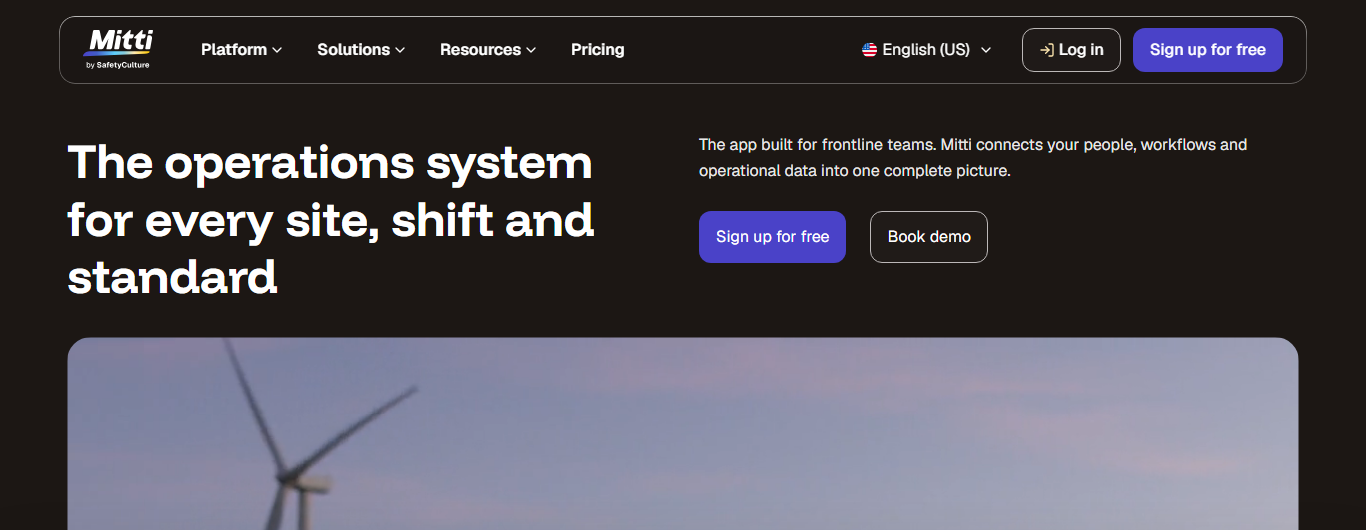
\includegraphics[width=0.85\linewidth]{Figures/cmp_safetyculture.png}
\caption{SafetyCulture (Mitti) платформын нүүр хуудас}
\label{fig:cmpsc}
\end{figure}

\subsection{Weekdone}
Weekdone нь OKR зорилго болон долоо хоногийн төлөвлөгөө, үр дүн, саадыг бичүүлж, багийн тайланг нэгтгэдэг. Долоо хоногийн тайлангийн дадлыг сайн хэрэгжүүлсэн боловч 5S, аудитын хэрэгсэлгүй~\cite{weekdone}.
\begin{figure}[H]
\centering
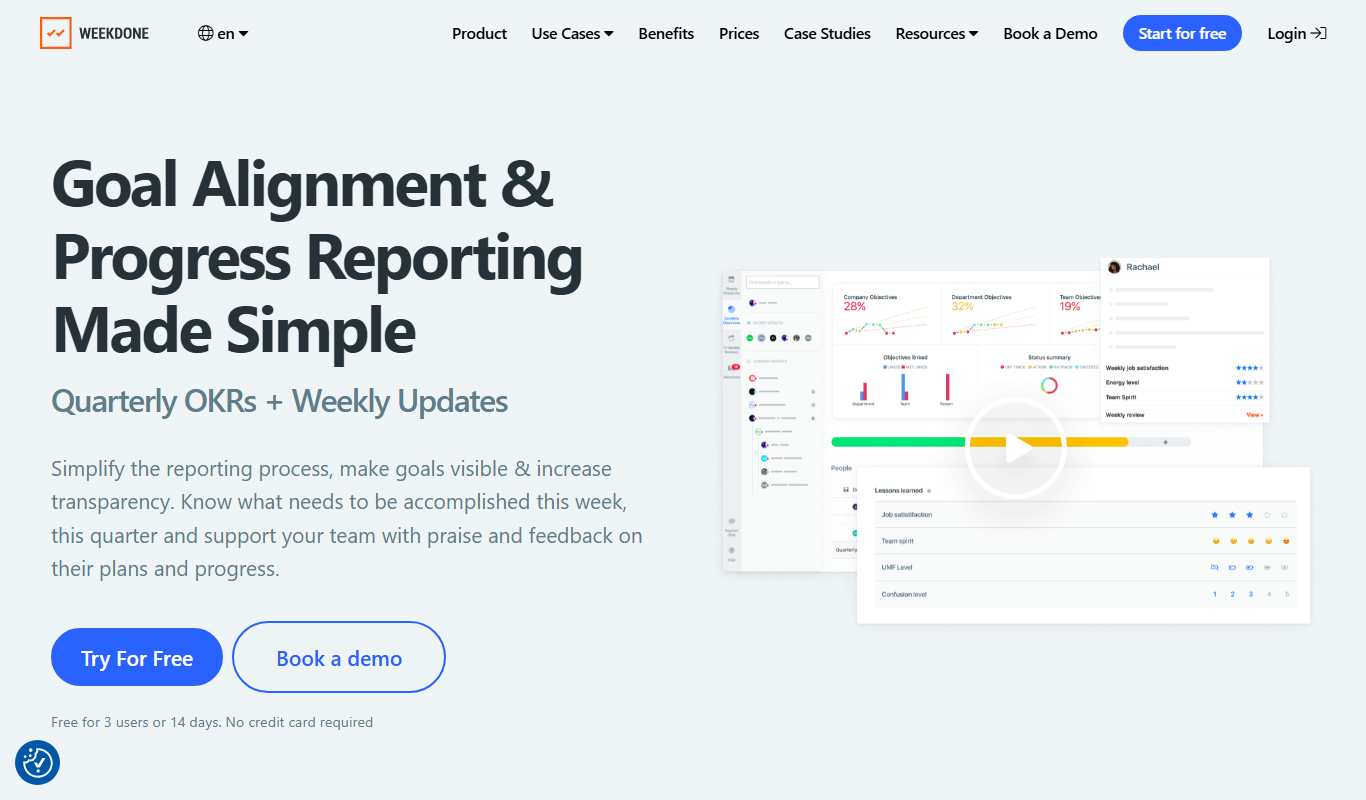
\includegraphics[width=0.85\linewidth]{Figures/cmp_weekdone.png}
\caption{Weekdone платформын нүүр хуудас}
\label{fig:cmpwd}
\end{figure}

\subsection{Asana}
Asana, Trello зэрэг ажлын удирдлагын системүүд ажил оноох, самбараар хянах, хугацаа сануулах боломжтой ч lean хэрэгсэл, аудит, талбайн удирдлага агуулдаггүй~\cite{asana}.
\begin{figure}[H]
\centering
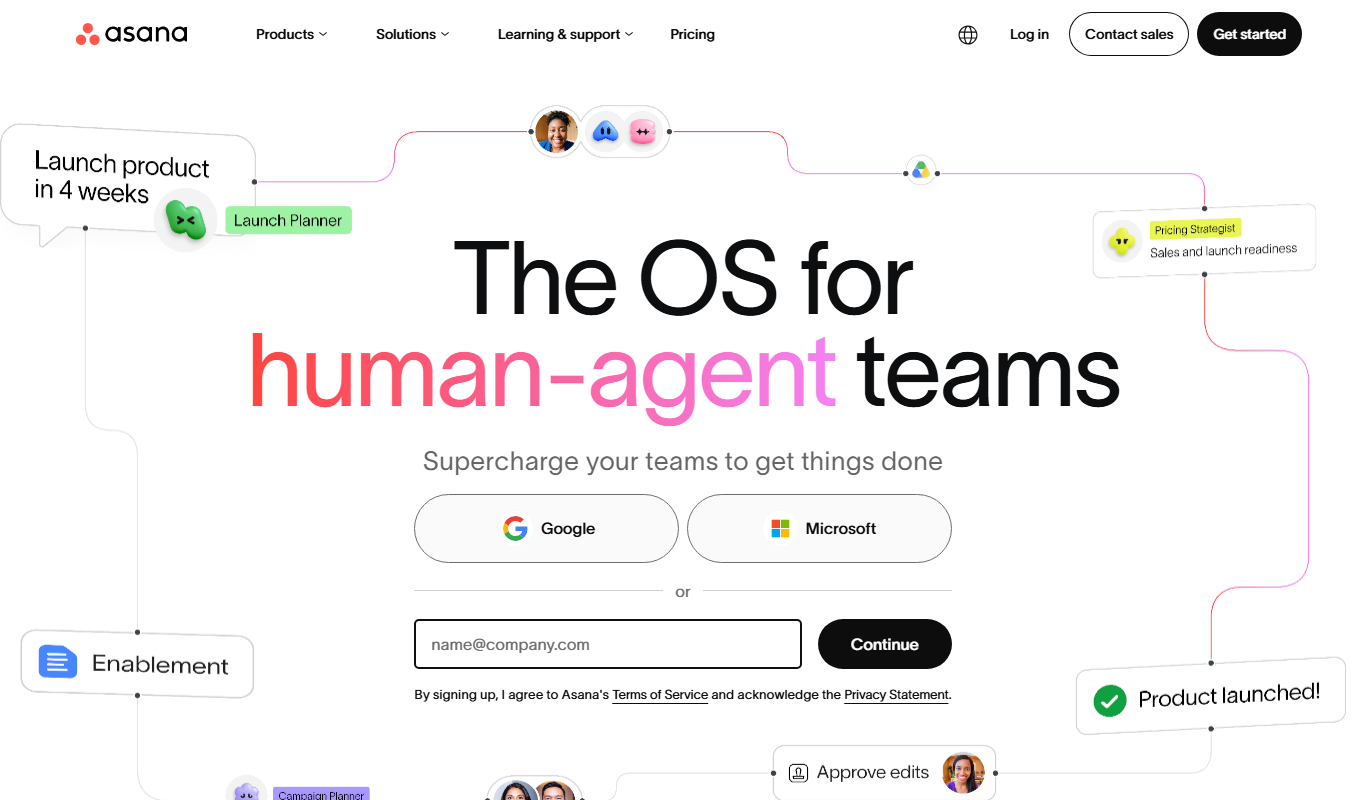
\includegraphics[width=0.85\linewidth]{Figures/cmp_asana.png}
\caption{Asana платформын нүүр хуудас}
\label{fig:cmpas}
\end{figure}

\subsection{KaiNexus}
KaiNexus нь тасралтгүй сайжруулалтын санаа, төслийг бүртгэж, үр нөлөөг хэмждэг платформ юм. Сайжруулалтын санааны урсгал сайн боловч аудит, сүлжээгүй горимгүй~\cite{kainexus}.
\begin{figure}[H]
\centering
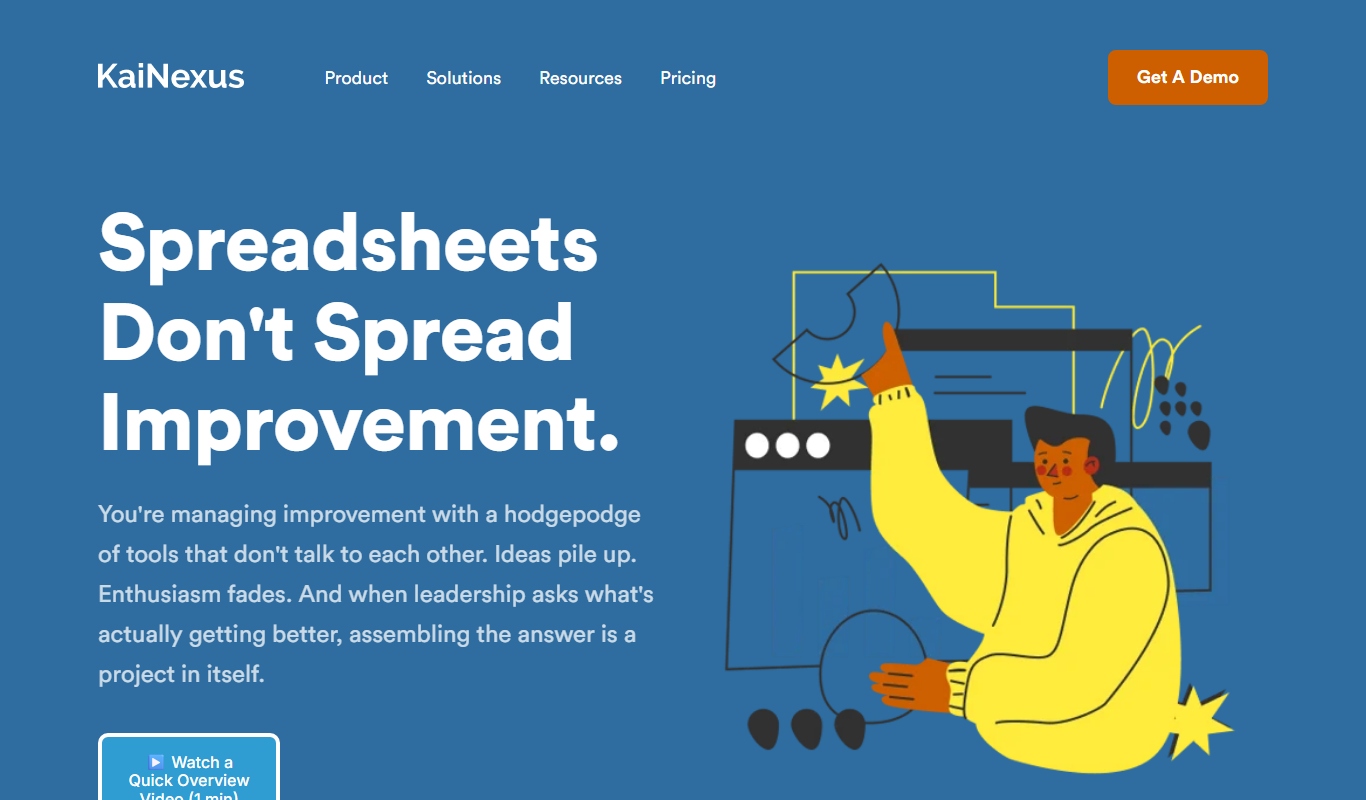
\includegraphics[width=0.85\linewidth]{Figures/cmp_kainexus.png}
\caption{KaiNexus платформын нүүр хуудас}
\label{fig:cmpkn}
\end{figure}

\subsection{Tervene}
Tervene нь шатлалт хурал, Gemba явалт, удирдагчийн стандарт ажил, харааны удирдлагын самбарыг цахимжуулсан үйлдвэрийн удирдлагын систем юм. Lean удирдлагын дадлыг хамгийн бүрэн хамардаг ч монгол хэлгүй, байгууллагын өөрийн серверт байршуулах боломжгүй~\cite{tervene}.
\begin{figure}[H]
\centering
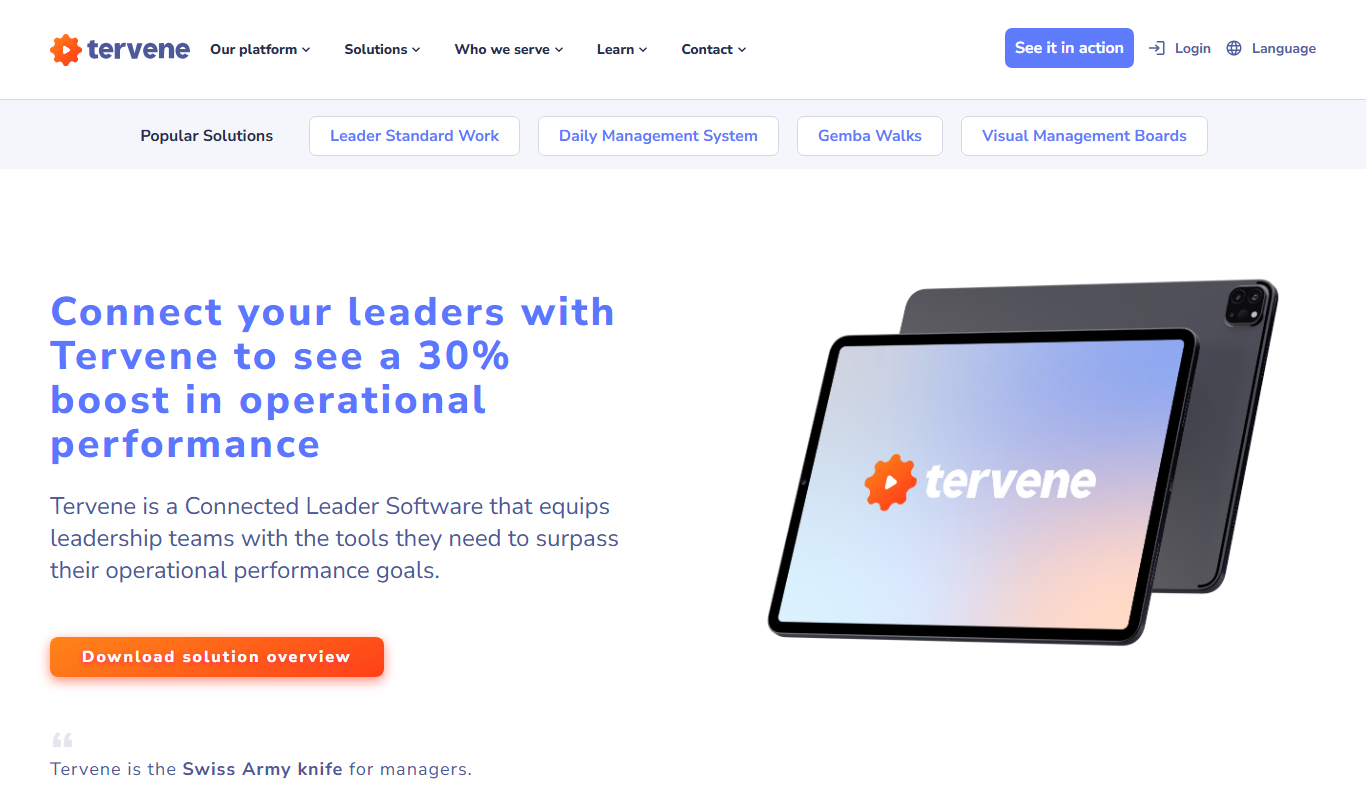
\includegraphics[width=0.85\linewidth]{Figures/cmp_tervene.png}
\caption{Tervene платформын нүүр хуудас}
\label{fig:cmptv}
\end{figure}

\subsection{Харьцуулалт ба SWOT шинжилгээ}


\begin{table}[H]
\centering
\caption{Ижил төстэй системийн боломжийн харьцуулалт}
\label{table:compare}
\begin{tabular}{|p{4.6cm}|c|c|c|c|c|c|}
\hline
\textbf{Боломж} & \rotatebox{90}{\textbf{SafetyCulture}} & \rotatebox{90}{\textbf{Weekdone}} & \rotatebox{90}{\textbf{Asana/Trello}} & \rotatebox{90}{\textbf{KaiNexus}} & \rotatebox{90}{\textbf{Tervene}} & \rotatebox{90}{\textbf{Энэ систем}} \\ \hline
Аудит, шалгах хуудас (утаснаас) & \yes & -- & -- & $\sim$ & \yes & \yes \\ \hline
Ажил оноох, хянах & $\sim$ & $\sim$ & \yes & \yes & \yes & \yes \\ \hline
Аудитаас автомат засах ажил & \yes & -- & -- & -- & $\sim$ & \yes \\ \hline
Сайжруулалтын санаа & -- & -- & -- & \yes & \yes & \yes \\ \hline
Өдөр тутмын хурлын самбар & -- & -- & -- & $\sim$ & \yes & \yes \\ \hline
Долоо хоногийн тайлан & -- & \yes & -- & -- & -- & \yes \\ \hline
Gemba явалтын бүртгэл & $\sim$ & -- & -- & -- & \yes & \yes \\ \hline
Сарын тайлан автоматаар & $\sim$ & $\sim$ & -- & $\sim$ & $\sim$ & \yes \\ \hline
Сүлжээгүй горим & \yes & -- & $\sim$ & -- & -- & \yes \\ \hline
Монгол хэл, өөрийн серверт & -- & -- & -- & -- & -- & \yes \\ \hline
\end{tabular}

\smallskip
{\small \yes -- бүрэн, $\sim$ -- хэсэгчлэн, -- -- байхгүй}
\end{table}

Хүснэгт~\ref{table:compare}-аас харахад SafetyCulture нь аудит, сүлжээгүй горимоороо, Weekdone нь долоо хоногийн тайлангаараа, KaiNexus, Tervene нь сайжруулалт болон lean удирдлагын дадлаараа давуу боловч эдгээрийг нэг дор, монгол хэл дээр, байгууллагын өөрийн серверт байршуулах боломжтой шийдэл байхгүй. Мөн эдгээр нь хэрэглэгч тус бүрээр гадаад валютаар төлбөртэй тул дотоодын байгууллагад зардал өндөр. Эдгээр системийн шилдэг туршлагыг (офлайн аудит, хариуцагчтай засах ажил, хурлын самбар, долоо хоногийн сануулга) энэхүү системд нэгтгэн тусгав.


Судалгааны үр дүнд үндэслэн хөгжүүлэх системийн давуу, сул тал, боломж, аюулыг Хүснэгт~\ref{table:swot}-д нэгтгэв.

\begin{table}[H]
\centering
\caption{Хөгжүүлэх системийн SWOT шинжилгээ}
\label{table:swot}
\begin{tabular}{|p{7cm}|p{7cm}|}
\hline
\textbf{Давуу тал (S)} & \textbf{Сул тал (W)} \\ \hline
\begin{itemize}[leftmargin=*,nosep]
\item Аудит, ажил, lean дадал нэг системд
\item Аудитаас засах ажил автоматаар үүснэ
\item Сүлжээгүй горим, монгол хэл
\item Өөрийн серверт байршуулах боломж
\end{itemize}
&
\begin{itemize}[leftmargin=*,nosep]
\item Хэрэглэгчийн бодит туршлага бага
\item Push мэдэгдэл хараахан байхгүй
\item Нэг хөгжүүлэгчтэй, дэмжлэгийн нөөц хязгаарлагдмал
\end{itemize}
\\ \hline
\textbf{Боломж (O)} & \textbf{Аюул (T)} \\ \hline
\begin{itemize}[leftmargin=*,nosep]
\item 5S, lean нэвтрүүлж буй байгууллага олон
\item Тайлан бэлтгэх цаг хэмнэх хэрэгцээ өндөр
\item AI ашиглан тайлан ноороглох
\end{itemize}
&
\begin{itemize}[leftmargin=*,nosep]
\item Гадаадын том системүүдтэй өрсөлдөх
\item Байгууллагын цахим шилжилтэд эсэргүүцэл
\item Хувийн мэдээллийн аюулгүй байдлын эрсдэл
\end{itemize}
\\ \hline
\end{tabular}
\end{table}

%-------------------------------------------------------------------------------
\section{Хэрэглэгчийн судалгаа}
% TODO: 5S, lean хэрэглэдэг байгууллагуудын ажилтнуудаас Google Form-оор судалгаа авч, үр дүнгийн графикуудыг
% Figures/survey*.png болгон энд оруулна. Үр дүнг зохиож бичихгүй.
Системийн шаардлагыг баталгаажуулах зорилгоор 5S, lean аргачлал хэрэглэдэг байгууллагуудын ажилтнуудаас онлайн асуулга авна. Асуулгын гол асуултууд:
\begin{enumerate}
    \item Та ажлын даалгаврыг голчлон ямар хэлбэрээр авдаг вэ? (ам, чат, имэйл, цаас, систем)
    \item 5S аудитын шалгах хуудсыг ямар хэлбэрээр бөглөдөг вэ?
    \item Аудитаар илэрсэн дутагдал засагдсан эсэхийг хэрхэн хянадаг вэ?
    \item Сарын тайлан бэлтгэхэд дунджаар хэдэн цаг зарцуулдаг вэ?
    \item Ажлын байранд интернэт тасалддаг уу?
    \item Сайжруулалтын санаагаа хаана, хэрхэн илэрхийлдэг вэ? Хариу авдаг уу?
    \item Ажлын системийг гар утаснаас ашиглах хэрэгцээ хэр байна вэ?
\end{enumerate}
Асуулгыг 2026 оны 10-р сард Google Forms-оор авч, хариултыг асуулт бүрээр график болгон нэгтгэнэ. Үр дүнг хоёрдугаар үзлэгт энэ хэсэгт тусгаж, шаардлагын жагсаалт болон тэдгээрийн эрэмбийг (Хүснэгт~\ref{table:fr}) шаардлагатай бол шинэчилнэ. Мөн туршилтын ажиллагааны төгсгөлд хэрэглэгчдээс SUS асуулга~\cite{brooke} авч, системийн хэрэглэхэд хялбар байдлыг 100 онооны хэмжүүрээр үнэлнэ.

%-------------------------------------------------------------------------------
\section{Системд тохирсон программ хангамжийн аргачлал}
Хөгжүүлэлтэд давталттай, өсөн нэмэгдэх (iterative and incremental) аргачлалыг сонгов~\cite{sommerville}. Захиалагчийн шаардлага эхнээсээ бүрэн тодорхой бус, туршилтын явцад өөрчлөгдөх магадлалтай тул давталт бүр нэг хэрэгцээг бүрэн (өгөгдлийн сан, API, вэб, гар утас, тест) хэрэгжүүлж, ажиллах хувилбар гаргана. Давталт бүр дараах алхмаас бүрдэнэ:
\begin{enumerate}[nosep]
    \item шаардлагыг тодорхойлох,
    \item зохиомжлох (өгөгдлийн загвар, API),
    \item хэрэгжүүлэх,
    \item автомат тест бичиж шалгах,
    \item захиалагчтай хянаж, дараагийн давталтыг төлөвлөх.
\end{enumerate}
Код бүрийг автомат тестээр хамгаалж, өөрчлөлт хийх бүрт бүх тестийг ажиллуулснаар өмнөх боломжуудыг эвдэхээс сэргийлнэ~\cite{beck}. Чанарын үзүүлэлтийг ISO/IEC 25010 стандартын функциональ тохирол, найдвартай байдал, хэрэглэхэд хялбар байдал, аюулгүй байдал, засварлагдах чанар гэсэн шинжүүдээр тодорхойлов~\cite{iso25010}.

%-------------------------------------------------------------------------------
\section{Технологийн тухай}
Технологийг хөгжүүлэлтийн хурд, нэг хэл дээр ажиллах боломж, урт хугацааны дэмжлэг, туршлага гэсэн шалгуураар сонгов.

\subsection{Front-End хөгжүүлэлтэд ашиглах технологиуд}
\begin{itemize}
    \item \textbf{React 18} -- компонентод суурилсан хэрэглэгчийн интерфейсийн сан~\cite{react}. Экосистем том, TypeScript-тэй сайн нийцдэг.
    \item \textbf{Vite} -- хурдан хөгжүүлэлтийн сервер ба бүтээх хэрэгсэл.
    \item \textbf{Tailwind CSS} -- utility класст суурилсан загварчлал; бараан горим, гар утасны дэлгэцэд тохируулахад хялбар.
    \item \textbf{i18next} -- монгол, англи хэлний орчуулга.
\end{itemize}

\subsection{Back-End хөгжүүлэлтэд ашиглах технологиуд}
\begin{itemize}
    \item \textbf{NestJS 11} -- TypeScript дээрх модульчлагдсан сервер талын фреймворк~\cite{nestjs}. Dependency injection, guard-аар эрх шалгах, cron үйлдлийг дэмждэг.
    \item \textbf{PostgreSQL} -- харилцааны өгөгдлийн сан~\cite{postgres}. Гадаад түлхүүрээр бүрэн бүтэн байдлыг хангаж, JSONB төрлөөр уян хатан өгөгдөл (5S бүс, шалгах хуудас) хадгална.
    \item \textbf{TypeORM} -- объект-харилцааны буулгалт (ORM); схемийн өөрчлөлтийг migration файлаар хувилбарчилна.
    \item \textbf{JWT} -- төлөвгүй нэвтрэлт; вэб, гар утас хоёрт ижил ажиллана~\cite{jwt}.
    \item \textbf{Docker Compose} -- nginx, API, PostgreSQL-ийг нэг тохиргоогоор байршуулна.
\end{itemize}

\subsection{Гар утасны хөгжүүлэлтэд ашиглах технологиуд}
\begin{itemize}
    \item \textbf{Flutter (Dart)} -- нэг кодоор Android, iOS аппыг бүтээх хүрээ~\cite{flutter}.
    \item \textbf{Provider} -- төлөв удирдлага; \textbf{Dio} -- HTTP клиент.
    \item \textbf{SharedPreferences} -- сүлжээгүй үед бүртгэлийн дарааллыг (outbox) хадгална.
\end{itemize}

\begin{table}[H]
\centering
\caption{Технологийн сонголт ба харьцуулсан хувилбарууд}
\label{table:tech}
\begin{tabular}{|p{2.4cm}|p{3.2cm}|p{2.8cm}|p{5.2cm}|}
\hline
\textbf{Давхарга} & \textbf{Сонгосон} & \textbf{Хувилбар} & \textbf{Үндэслэл} \\ \hline
Backend & NestJS 11 & Express, Django & Модульчлагдсан бүтэц, guard, вэбтэй нэг хэл \\ \hline
Өгөгдлийн сан & PostgreSQL & MySQL, MongoDB & Бүрэн бүтэн байдал, JSONB, migration \\ \hline
Вэб & React 18 & Angular, Vue & Компонент, экосистем, хурд \\ \hline
Гар утас & Flutter & React Native & Нэг код, тогтвортой гүйцэтгэл, widget тест \\ \hline
Байршуулалт & Docker Compose & Шууд суулгах & Орчин ижил, өөрийн серверт хялбар \\ \hline
\end{tabular}
\end{table}

\section*{Бүлгийн дүгнэлт}
Энэ бүлэгт бүтээмжийн аргачлалуудын онолыг судалж, тэдгээрийг дадал болгоход сануулга, хяналтын механизм шаардлагатайг тодорхойлов. Ижил төстэй таван системийг харьцуулж, SWOT шинжилгээ хийж, аудит, ажлын удирдлага, lean дадлыг нэг дор, монгол хэл дээр нэгтгэсэн шийдэл байхгүйг тогтоов. Мөн давталттай хөгжүүлэлтийн аргачлал, NestJS, PostgreSQL, React, Flutter технологийг сонгосон үндэслэлээ тайлбарлав.

% Бүлэг 2

\chapter{Системийн шинжилгээ}
\label{Chapter2}

% Юзкейсийн тодорхойлолтын хүснэгт: {нэр}{ID}{үндсэн}{нэмэлт}{товч}{өмнөх}{урсгал}{дараах}{алтернатив}
\newcommand{\usecase}[9]{%
\begin{longtable}{|p{3.4cm}|p{11.2cm}|}
\caption{#1 юзкейсийн тодорхойлолт}\label{table:uc#2}\\ \hline
\textbf{Юзкейс:} & #1 \\ \hline
\textbf{ID:} & UC-#2 \\ \hline
\textbf{Үүсгэсэн:} & \shortname \\ \hline
\textbf{Үүсгэсэн огноо:} & 2026.09.29 \\ \hline
\textbf{Үндсэн тоглогч:} & #3 \\ \hline
\textbf{Нэмэлт тоглогч:} & #4 \\ \hline
\textbf{Товч тайлбар:} & #5 \\ \hline
\textbf{Өмнөх нөхцөл:} & #6 \\ \hline
\textbf{Үндсэн урсгал:} & #7 \\ \hline
\textbf{Дараах нөхцөл:} & #8 \\ \hline
\textbf{Алтернатив урсгал:} & #9 \\ \hline
\end{longtable}}

%-------------------------------------------------------------------------------
\section{Системийн үйл ажиллагаа}
Одоогийн байдлаар 5S, lean аргачлал хэрэглэдэг байгууллагуудад аудитын шалгах хуудас цаасаар бөглөгдөж, дараа нь хүснэгтэд шивэгдэнэ; ажлын даалгавар ам болон чатаар өгөгдөнө; сарын тайланг хэлтэс бүрийн мэдээллээс гараар нэгтгэнэ. Шинэ систем эдгээр урсгалыг нэг өгөгдлийн сан дээр нэгтгэж, мэдээллийг үүссэн газарт нь (цех дээр, гар утаснаас) бүртгэх боломж олгоно. Системийн үйл ажиллагааг хэрэглэгчийн дүрээр тайлбарлавал:

\paragraph{}\textbf{Ажилтан}: өөрт оноосон ажлыг ``хоцорсон, өнөөдөр, энэ долоо хоногт'' гэсэн дарааллаар харж, нэг товшилтоор дуусгана. Өдрийн бүртгэл, долоо хоногийн тайлан бичнэ. Талбайн QR шошгыг гар утсаар уншуулж 5S аудит хийж, улаан шошго, дутагдлыг зурагтай бүртгэнэ. Сайжруулалтын санаа илгээж, хариуг нь мэдэгдлээр авна. Сүлжээгүй үед хийсэн бүртгэл утсанд хадгалагдана.

\paragraph{}\textbf{Менежер}: ажилтны бүх үйлдлийг хийхээс гадна төсөл, ажил үүсгэж хариуцагч, хугацаа онооно. Явцын самбар, өглөөний хурлын самбараас хоцорсон, хариуцагчгүй ажлыг харна. Gemba явалт бүртгэж, санааг хянана. Сарын тайлангийн тойм бичвэрийг бичиж батална.

\paragraph{}\textbf{Админ}: менежерийн бүх үйлдлийг хийхээс гадна хэрэглэгч урьж, эрх олгоно; хэлтэс, 5S талбай, аудитын загвар, байгууллагын тохиргоог удирдана.

\paragraph{}\textbf{Систем (цагийн хуваарь)}: өглөө бүр дуусах, хоцорсон ажлын сануулга илгээнэ; талбайн аудитын давтамжийн дагуу аудитын ажил үүсгэнэ; сар дуусахад тайланг хааж архивлана.

%-------------------------------------------------------------------------------
\section{Системийг ашиглах хэрэглэгчид}
Хэрэглэгчийн дүрүүд үүрлэсэн (ажиглагч $\subset$ ажилтан $\subset$ менежер $\subset$ админ) бөгөөд дээд дүр доод дүрийн бүх эрхийг өвлөнө (Хүснэгт~\ref{table:roles}).

\begin{table}[H]
\centering
\caption{Хэрэглэгчийн дүр ба эрх}
\label{table:roles}
\begin{tabular}{|p{2.8cm}|p{4.4cm}|p{7.2cm}|}
\hline
\textbf{Дүр} & \textbf{Тайлбар} & \textbf{Гол эрхүүд} \\ \hline
Ажиглагч & Удирдлага, зөвлөх зэрэг зөвхөн хардаг хэрэглэгч & Ажил, аудит, тайлан, санаа унших; мэдэгдэл унших \\ \hline
Ажилтан & Цех, оффисын ажилтан & Өөрт оноосон ажил шинэчлэх, өдрийн бүртгэл, аудит, улаан шошго, санаа, долоо хоногийн тайлан \\ \hline
Менежер & Хэлтэс, багийн удирдлага & Ажил, төсөл үүсгэх, оноох; сарын тайлан хаах; санаа хянах; Gemba явалт; хэрэглэгч урих \\ \hline
Админ & Байгууллагын систем хариуцагч & Хэрэглэгч, хэлтэс, талбай, загвар, тохиргоо; өөрөөсөө доод түвшний эрх олгох \\ \hline
\end{tabular}
\end{table}

%-------------------------------------------------------------------------------
\section{Функциональ шаардлага}
Функциональ шаардлагыг MoSCoW аргаар эрэмбэлэв (M -- заавал, S -- байх ёстой, C -- байж болно).

\begin{longtable}{|p{1.4cm}|p{9.6cm}|p{2.4cm}|c|}
\caption{Функциональ шаардлага}\label{table:fr}\\ \hline
\textbf{Код} & \textbf{Шаардлага} & \textbf{Дүр} & \textbf{Эр.} \\ \hline
\endfirsthead
\hline
\textbf{Код} & \textbf{Шаардлага} & \textbf{Дүр} & \textbf{Эр.} \\ \hline
\endhead
FR-01 & Хэрэглэгч и-мэйл, нууц үгээр нэвтэрч, эрхийнхээ хүрээнд системийг ашиглана & Бүгд & M \\ \hline
FR-02 & Админ хэрэглэгчийг урилгаар нэмж, өөрөөсөө доод түвшний эрх олгоно & Админ & M \\ \hline
FR-03 & Менежер ажил үүсгэж, хариуцагч, хугацаа, ач холбогдол онооно & Менежер & M \\ \hline
FR-04 & Ажилтан өөрт оноосон ажлыг хоцорсон, өнөөдөр, энэ долоо хоног гэж эрэмбэлж харна & Ажилтан & M \\ \hline
FR-05 & Ажил оноогдоход болон өглөө бүр дуусах, хоцорсон ажлын талаар мэдэгдэл ирнэ & Ажилтан & M \\ \hline
FR-06 & Менежер 5S талбайн зураг зурж, бүс бүрт хариуцагч, стандарт зураг, аудитын давтамж онооно & Менежер & M \\ \hline
FR-07 & Ажилтан бүсийн QR шошгыг уншуулж, шалгах хуудсаар аудит хийнэ & Ажилтан & M \\ \hline
FR-08 & Аудитын оноо босгоос доош бол бүсийн хариуцагчид засах ажил автоматаар үүснэ & Систем & M \\ \hline
FR-09 & Ажилтан улаан шошго болон дутагдлыг зурагтай бүртгэнэ & Ажилтан & M \\ \hline
FR-10 & Ажилтан өдрийн бүртгэл (юу хийсэн, дараа нь юу хийх) хөтөлнө & Ажилтан & M \\ \hline
FR-11 & Ажилтан долоо хоногийн тайлан бичнэ; пүрэв, баасан гарагт сануулга гарна & Ажилтан & S \\ \hline
FR-12 & Сарын тайлан бүртгэлээс автоматаар бүрдэж, тогтсон өдөр хаагдан архивлагдана & Систем & M \\ \hline
FR-13 & Хагас жилийн, жилийн тайлан хаагдсан сарын тайлангаас нэгтгэгдэнэ & Менежер & S \\ \hline
FR-14 & Менежер сарын тайлангийн тойм бичвэрийг AI-аар ноороглуулж, засаад батална & Менежер & C \\ \hline
FR-15 & Өглөөний хурлын самбар өчигдөр, өнөөдөр, анхаарах зүйл, 5S, Gemba-г харуулна & Менежер & S \\ \hline
FR-16 & Менежер Gemba явалт бүртгэж, дараагийн алхам бүр ажил болно & Менежер & S \\ \hline
FR-17 & Ажилтан сайжруулалтын санаа илгээж, менежер хянаж хариу өгнө & Ажилтан, менежер & S \\ \hline
FR-18 & Гар утасны апп сүлжээгүй үед хийсэн өөрчлөлтийг хадгалж, дараа илгээнэ & Ажилтан & M \\ \hline
FR-19 & Систем монгол, англи хэлээр ажиллана & Бүгд & M \\ \hline
FR-20 & Байгууллагын үйл ажиллагааны түүх (аудитын бүртгэл, архив) хадгалагдана & Админ & S \\ \hline
FR-21 & Хэрэглэгч бүртгэлээ устгах хүсэлт гаргана & Бүгд & S \\ \hline
FR-22 & Удирдлага туршилтын үзүүлэлтүүдийг (K1--K6, \ref{sec:kpi}-р хэсэг) сар, долоо хоногоор харна & Менежер & S \\ \hline
\end{longtable}

%-------------------------------------------------------------------------------
\section{Функциональ бус шаардлага}
\begin{longtable}{|p{1.6cm}|p{3.2cm}|p{9.6cm}|}
\caption{Функциональ бус шаардлага (ISO/IEC 25010)}\label{table:nfr}\\ \hline
\textbf{Код} & \textbf{Шинж} & \textbf{Шаардлага} \\ \hline
\endfirsthead
\hline
\textbf{Код} & \textbf{Шинж} & \textbf{Шаардлага} \\ \hline
\endhead
NFR-01 & Аюулгүй байдал & Нууц үг hash-лагдаж хадгалагдана; бүх хүсэлт JWT-ээр баталгаажна; эрхийг сервер тал дээр шалгана \\ \hline
NFR-02 & Аюулгүй байдал & Байгууллага бүрийн өгөгдөл тусгаарлагдана; нэг байгууллага нөгөөгийнхийг харахгүй \\ \hline
NFR-03 & Хэрэглэхэд хялбар & WCAG 2.1 AA хүртээмж~\cite{wcag}; SUS оноо 68-аас дээш~\cite{brooke} \\ \hline
NFR-04 & Хэрэглэхэд хялбар & Гар утсанд нэг гараар ашиглах, том үсэг, бараан горимд зохицно \\ \hline
NFR-05 & Найдвартай байдал & Сүлжээ тасрахад өгөгдөл алдагдахгүй; давхар илгээлтээс сэргийлнэ \\ \hline
NFR-06 & Гүйцэтгэл & Гол хуудас энгийн сүлжээнд 2 секундээс бага хугацаанд ачаална \\ \hline
NFR-07 & Засварлагдах чанар & Өгөгдлийн сангийн өөрчлөлт migration-оор; автомат тестийн хамрах хүрээ \\ \hline
NFR-08 & Зөөвөрлөх чанар & Docker-оор аль ч Linux сервер дээр байршина \\ \hline
NFR-09 & Нууцлал & AI үйлчилгээ рүү зөвхөн нэргүй, нэгдсэн тоо баримт илгээгдэнэ \\ \hline
NFR-10 & Цаг хугацаа & Огноо, сануулга байгууллагын цагийн бүсээр (Asia/Ulaanbaatar) тооцогдоно \\ \hline
\end{longtable}

%-------------------------------------------------------------------------------
\section{Use Case диаграмм}
Зураг~\ref{fig:usecase}-т системийн оролцогчид болон тэдгээрийн гүйцэтгэх гол use-case-уудыг харуулав. Менежер ажилтны, админ менежерийн бүх use-case-ийг өвлөнө.

\begin{figure}[H]
\centering
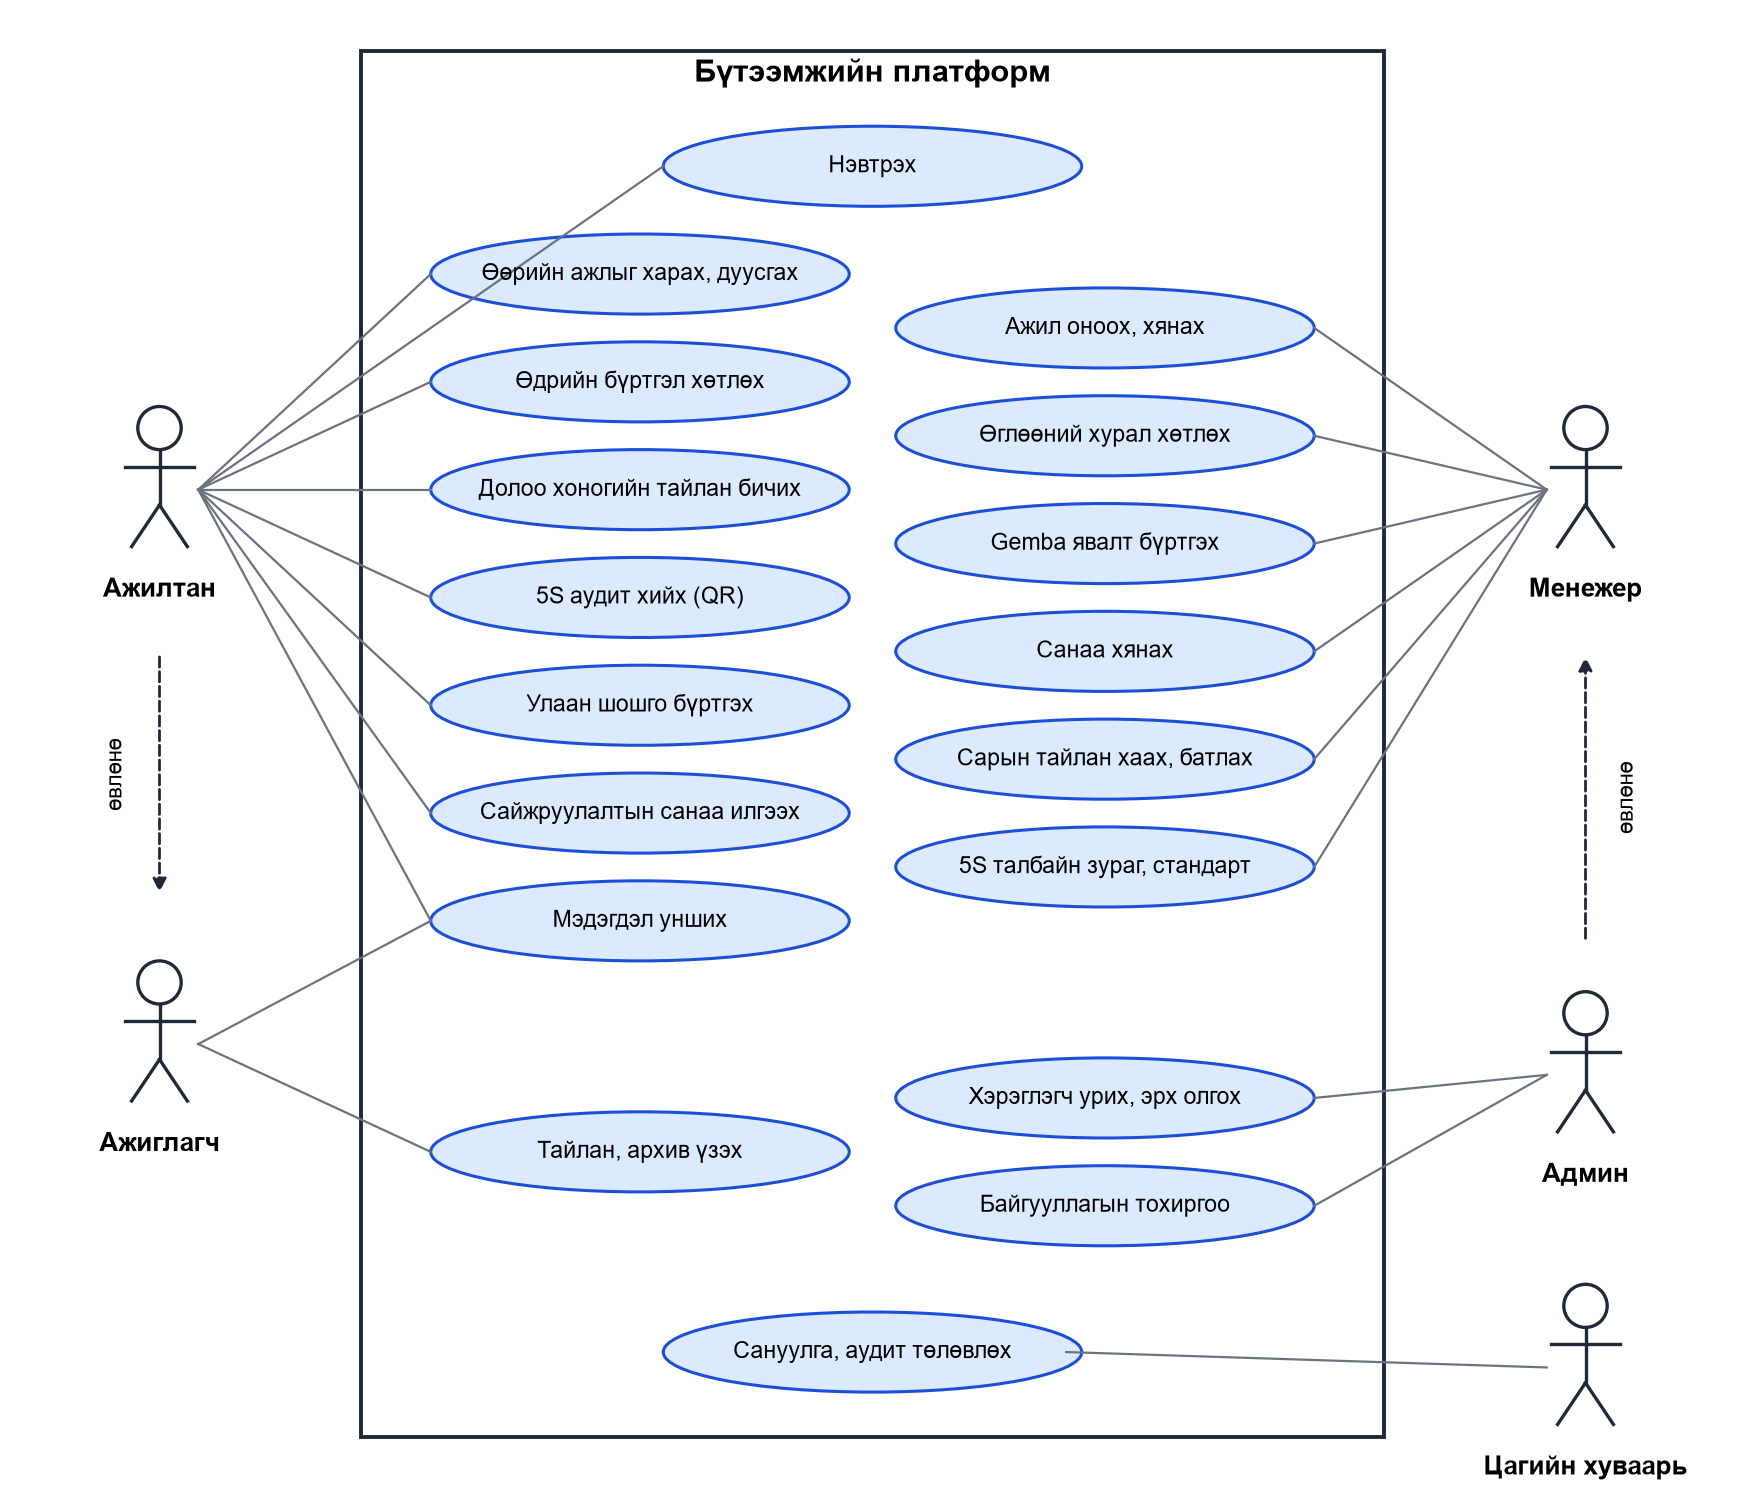
\includegraphics[width=\linewidth]{Figures/usecase.png}
\caption{Юзкейс диаграмм}
\label{fig:usecase}
\end{figure}

%-------------------------------------------------------------------------------
\section{Юзкейс диаграммын тодорхойлолт}
Гол use-case-уудын тодорхойлолтыг Хүснэгт~\ref{table:uc01}--\ref{table:uc09}-д харуулав~\cite{cockburn}.

\usecase{Нэвтрэх}{01}{Хэрэглэгч}{Байхгүй}
{Бүртгэлтэй хэрэглэгч системд нэвтэрнэ.}
{Хэрэглэгч идэвхтэй бүртгэлтэй байх.}
{1. Хэрэглэгч и-мэйл, нууц үгээ оруулж ``Нэвтрэх'' дарна.\par
 2. Систем и-мэйлээр хэрэглэгчийг хайж, нууц үгийн hash-ийг шалгана.\par
 3. Систем access, refresh токен үүсгэнэ.\par
 4. Систем хэрэглэгчийн эрхэд тохирсон нүүр хуудсыг харуулна.}
{Хэрэглэгч нэвтэрсэн, токен хадгалагдсан байна.}
{2а. Нууц үг буруу эсвэл бүртгэл идэвхгүй бол алдааны мэдэгдэл харуулна.}

\usecase{5S аудит хийх}{02}{Ажилтан}{Систем}
{Бүсийн 5S түвшинг шалгах хуудсаар хэмжиж, дутагдлыг бүртгэнэ.}
{Хэрэглэгч нэвтэрсэн; бүс нь аудитын загвартай; audits:create эрхтэй.}
{1. Ажилтан бүсийн QR шошгыг уншуулна.\par
 2. Систем бүсийн шалгах хуудас, стандарт зургийг харуулна.\par
 3. Ажилтан асуулт бүрт оноо эсвэл тийм/үгүй хариулт өгч, шаардлагатай бол зураг хавсаргана.\par
 4. Ажилтан ``Дуусгах'' дарна.\par
 5. Систем оноог тооцоолж хадгалж, бүсийн сүүлийн оноог шинэчилнэ.\par
 6. Оноо 85\%-иас доош бол систем бүсийн хариуцагчид засах ажил үүсгэж мэдэгдэнэ.}
{Аудитын бүртгэл, бүсийн оноо, шаардлагатай бол засах ажил үүссэн байна.}
{5а. Сүлжээгүй бол аудит утсанд хадгалагдаж, сүлжээ сэргэхэд илгээгдэнэ.\par
 6а. Тухайн аудитаас ажил үүссэн бол давхар үүсгэхгүй.}

\usecase{Ажил оноох}{03}{Менежер}{Ажилтан}
{Ажлыг хариуцагчтай, хугацаатай оноож, биелэлтийг хянана.}
{Менежер tasks:create эрхтэй; хариуцагч идэвхтэй хэрэглэгч.}
{1. Менежер ажлын нэр, тайлбар, хариуцагч, хугацаа, ач холбогдлыг оруулна.\par
 2. Систем эрхийг шалгаж, ажлыг хадгална.\par
 3. Систем хариуцагчид мэдэгдэл илгээнэ.\par
 4. Ажилтан ажлын төлвийг ``хийгдэж байна'', ``дууссан'' болгоно.\par
 5. Менежер явцын самбараас биелэлтийг харна.}
{Ажил хариуцагчтай, хугацаатай бүртгэгдсэн байна.}
{2а. Эрхгүй бол 403 алдаа буцаана.\par
 4а. Хугацаа хэтэрвэл ажил ``хоцорсон'' бүлэгт орж өглөөний сануулгад багтана.}

\usecase{Сарын тайлан хаах}{04}{Систем (цагийн хуваарь)}{Менежер}
{Сарын үр дүнг автоматаар нэгтгэж, өөрчлөгдөхгүй хувилбараар архивлана.}
{Байгууллагын тохиргоонд сар хаах өдөр тодорхойлогдсон.}
{1. Систем цаг тутам байгууллага бүрийн цагийн бүсээр хаах өдөр болсон эсэхийг шалгана.\par
 2. Өнгөрсөн сар хаагдаагүй бол тухайн сарын бүртгэлүүдийг хуулбарлан хадгална.\par
 3. Менежер тайланг нээж, тойм бичвэр бичих эсвэл AI-аар ноороглуулна.\par
 4. Менежер бичвэрийг засаад батална.}
{Хаагдсан, архивлагдсан сарын тайлан бий болно.}
{1а. Сервер тухайн өглөө ажиллаагүй бол дараагийн ажиллалтаар хаана.\par
 3а. AI тохируулаагүй бол менежер гараар бичнэ.}

\usecase{Gemba явалт бүртгэх}{05}{Менежер}{Систем}
{Цех дээр ажигласан зүйл, ярилцлагыг бүртгэж, дараагийн алхмыг ажил болгоно.}
{Хэрэглэгч gemba:walk эрхтэй.}
{1. Менежер бүс эсвэл газрыг сонгоно.\par
 2. Ажигласан зүйл, хийсэн ярилцлагаа бичнэ.\par
 3. Дараагийн алхам бүрт нэр, хариуцагч оруулна.\par
 4. Систем явалтыг хадгалж, алхам бүрээс ажил үүсгэнэ.}
{Gemba явалтын бүртгэл ба хариуцагчтай ажлууд үүснэ.}
{3а. Хариуцагч сонгоогүй бол ажил явалт хийсэн менежерт оноогдоно.}

\usecase{Сайжруулалтын санаа илгээх}{06}{Ажилтан}{Менежер}
{Ажилтны санааг бүртгэж, шийдвэрийг санал гаргагчид мэдэгдэнэ.}
{Ажилтан ideas:create, менежер ideas:review эрхтэй.}
{1. Ажилтан санааны гарчиг, тайлбар, зураг оруулж илгээнэ.\par
 2. Менежер санааг хянаж шийдвэр, хариу бичнэ.\par
 3. Систем санал гаргагчид мэдэгдэл илгээнэ.\par
 4. Батлагдсан санаанаас ажил үүснэ.}
{Санаа хариутай болж, шаардлагатай бол ажил үүснэ.}
{2а. Хянагдаагүй санаа өглөөний хурлын самбарт харагдана.}

\usecase{Долоо хоногийн тайлан бичих}{07}{Ажилтан}{Менежер}
{Долоо хоногийн үр дүн, төлөвлөгөө, саадыг товч бүртгэнэ.}
{Хэрэглэгч checkins:write эрхтэй.}
{1. Пүрэв, баасан гарагт тайлан бичээгүй ажилтанд сануулга гарна.\par
 2. Ажилтан хийсэн ажил, дараагийн төлөвлөгөө, саад бэрхшээлээ бичнэ.\par
 3. Систем хадгална.\par
 4. Менежер багийн тайлангуудыг нэг дор уншина.}
{Долоо хоногийн тайлан хадгалагдана.}
{2а. Сүлжээгүй бол утсанд хадгалагдана.}

\usecase{Өглөөний хурал хөтлөх}{08}{Менежер}{Ажилтан}
{Ээлжийн эхэнд багийн өчигдрийн үр дүн, өнөөдрийн ажил, анхаарах асуудлыг нэг дэлгэцээс хэлэлцэнэ.}
{Менежер нэвтэрсэн; хэлтэст ажилтнууд бүртгэлтэй.}
{1. Менежер ``Өглөөний хурал'' хуудсыг нээж, хэлтсээ сонгоно.\par
 2. Систем өчигдөр дууссан ажил, аудитын дундаж, өнөөдөр дуусах ажил, хоцорсон ба хариуцагчгүй ажил, стандартаас доош 5S бүс, хянагдаагүй санаа, Gemba-гийн биелэлтийг харуулна.\par
 3. Менежер хоцорсон ажлын хариуцагч, хугацааг хэлэлцэж шийдвэрлэнэ.\par
 4. Систем тоо баримтыг хоёр минут тутамд шинэчилнэ.}
{Баг өдрийн тэргүүлэх ажил, шийдвэр шаардсан асуудлаа тохирсон байна.}
{1а. Том дэлгэцэд бүтэн дэлгэцийн горимоор харуулна.}

\usecase{5S талбай, стандарт тохируулах}{09}{Админ, менежер}{Ажилтан}
{Байгууллагын талбайн зургийг зурж, бүс бүрт хариуцагч, стандарт зураг, аудитын давтамж онооно.}
{Хэрэглэгч zones:update эрхтэй.}
{1. Менежер талбайн зураг (давхар, бүс, объект)-ыг зурах эсвэл зураг оруулна.\par
 2. Бүс бүрт нэр, код, хариуцагч, стандарт зураг, аудитын шат, давтамжийг онооно.\par
 3. Систем өөрчлөлтийг хувилбараар хадгалж, бүс бүрийн QR шошгыг үүсгэнэ.\par
 4. Цагийн хуваарь давтамжийн дагуу аудитын ажил үүсгэнэ.}
{Бүсүүд хариуцагчтай, стандарттай, аудитын хуваарьтай болно.}
{3а. Өмнөх хувилбарыг сэргээх боломжтой.}

%-------------------------------------------------------------------------------
\section{Шаардлагын мөрдөх матриц}
Шаардлага бүр аль use-case-ээр хэрэгжиж, одоогийн байдлаар хаана хүрснийг Хүснэгт~\ref{table:trace}-д харуулав. Хэрэгжилтийг гурван түвшинд ялгав: \textbf{Код} -- системд хэрэгжсэн, \textbf{Тест} -- автомат тестээр баталгаажсан, \textbf{Туршилт} -- бодит байгууллагад ашиглаж хэмжсэн (\yes~бүрэн, $\sim$~хэсэгчлэн, --~хараахан үгүй).

\begin{longtable}{|p{1.3cm}|p{6.2cm}|p{1.6cm}|c|c|c|}
\caption{Шаардлагын мөрдөх матриц ба хэрэгжилтийн төлөв}\label{table:trace}\\ \hline
\textbf{Код} & \textbf{Шаардлага} & \textbf{Use-case} & \textbf{Код} & \textbf{Тест} & \textbf{Туршилт} \\ \hline
\endfirsthead
\hline
\textbf{Код} & \textbf{Шаардлага} & \textbf{Use-case} & \textbf{Код} & \textbf{Тест} & \textbf{Туршилт} \\ \hline
\endhead
FR-01 & Нэвтрэх, эрхийн хүрээ & UC-01 & \yes & \yes & -- \\ \hline
FR-02 & Урилга, эрх олгох & -- & \yes & \yes & -- \\ \hline
FR-03 & Ажил үүсгэх, оноох & UC-03 & \yes & \yes & -- \\ \hline
FR-04 & Ажлыг ач холбогдлоор харах & UC-03 & \yes & \yes & -- \\ \hline
FR-05 & Оноолт ба өглөөний мэдэгдэл & UC-03 & \yes & \yes & -- \\ \hline
FR-06 & 5S талбай, бүс, стандарт & UC-09 & \yes & \yes & -- \\ \hline
FR-07 & QR-ээр аудит хийх & UC-02 & \yes & \yes & -- \\ \hline
FR-08 & Аудитаас засах ажил & UC-02 & \yes & \yes & -- \\ \hline
FR-09 & Улаан шошго, зураг & UC-02 & \yes & \yes & -- \\ \hline
FR-10 & Өдрийн бүртгэл & UC-07 & \yes & \yes & -- \\ \hline
FR-11 & Долоо хоногийн тайлан, сануулга & UC-07 & \yes & \yes & -- \\ \hline
FR-12 & Сарын тайлан, хаалт, архив & UC-04 & \yes & \yes & -- \\ \hline
FR-13 & Хагас жил, жилийн тайлан & UC-04 & \yes & \yes & -- \\ \hline
FR-14 & AI тойм бичвэр & UC-04 & \yes & $\sim$ & -- \\ \hline
FR-15 & Өглөөний хурлын самбар & UC-08 & \yes & \yes & -- \\ \hline
FR-16 & Gemba явалт & UC-05 & \yes & \yes & -- \\ \hline
FR-17 & Сайжруулалтын санаа & UC-06 & \yes & \yes & -- \\ \hline
FR-18 & Сүлжээгүй горим & UC-02, 05, 07 & $\sim$ & \yes & -- \\ \hline
FR-19 & Монгол, англи хэл & бүгд & \yes & \yes & -- \\ \hline
FR-20 & Үйл ажиллагааны түүх, архив & UC-04 & \yes & \yes & -- \\ \hline
FR-21 & Бүртгэл устгах хүсэлт & -- & \yes & \yes & -- \\ \hline
FR-22 & KPI самбар (K1--K6) & UC-04, 08 & $\sim$ & -- & -- \\ \hline
\end{longtable}

FR-14-ийн AI дуудлагыг хиймэл хариугаар тестэлсэн бөгөөд бодит түлхүүрээр туршаагүй. FR-18-ийн сүлжээгүй горим нь бичих үйлдлүүдэд хэрэгжсэн, өгөгдлийг бүрэн офлайнаар унших нь хамрах хүрээнд ороогүй. Бүх шаардлагын ``Туршилт'' баганыг гуравдугаар үзлэгийн туршилтын ажиллагаагаар бөглөнө.

%-------------------------------------------------------------------------------
\section{Шинжилгээний класс диаграмм}
Зураг~\ref{fig:classA}-д системийн домэйн классууд, тэдгээрийн шинж чанар, хамаарлыг харуулав. Ажил (Task) нь аудит, Gemba явалт, санаанаас үүсэх бөгөөд sourceType, sourceId талбараар эх сурвалжаа хадгална.

\begin{figure}[H]
\centering
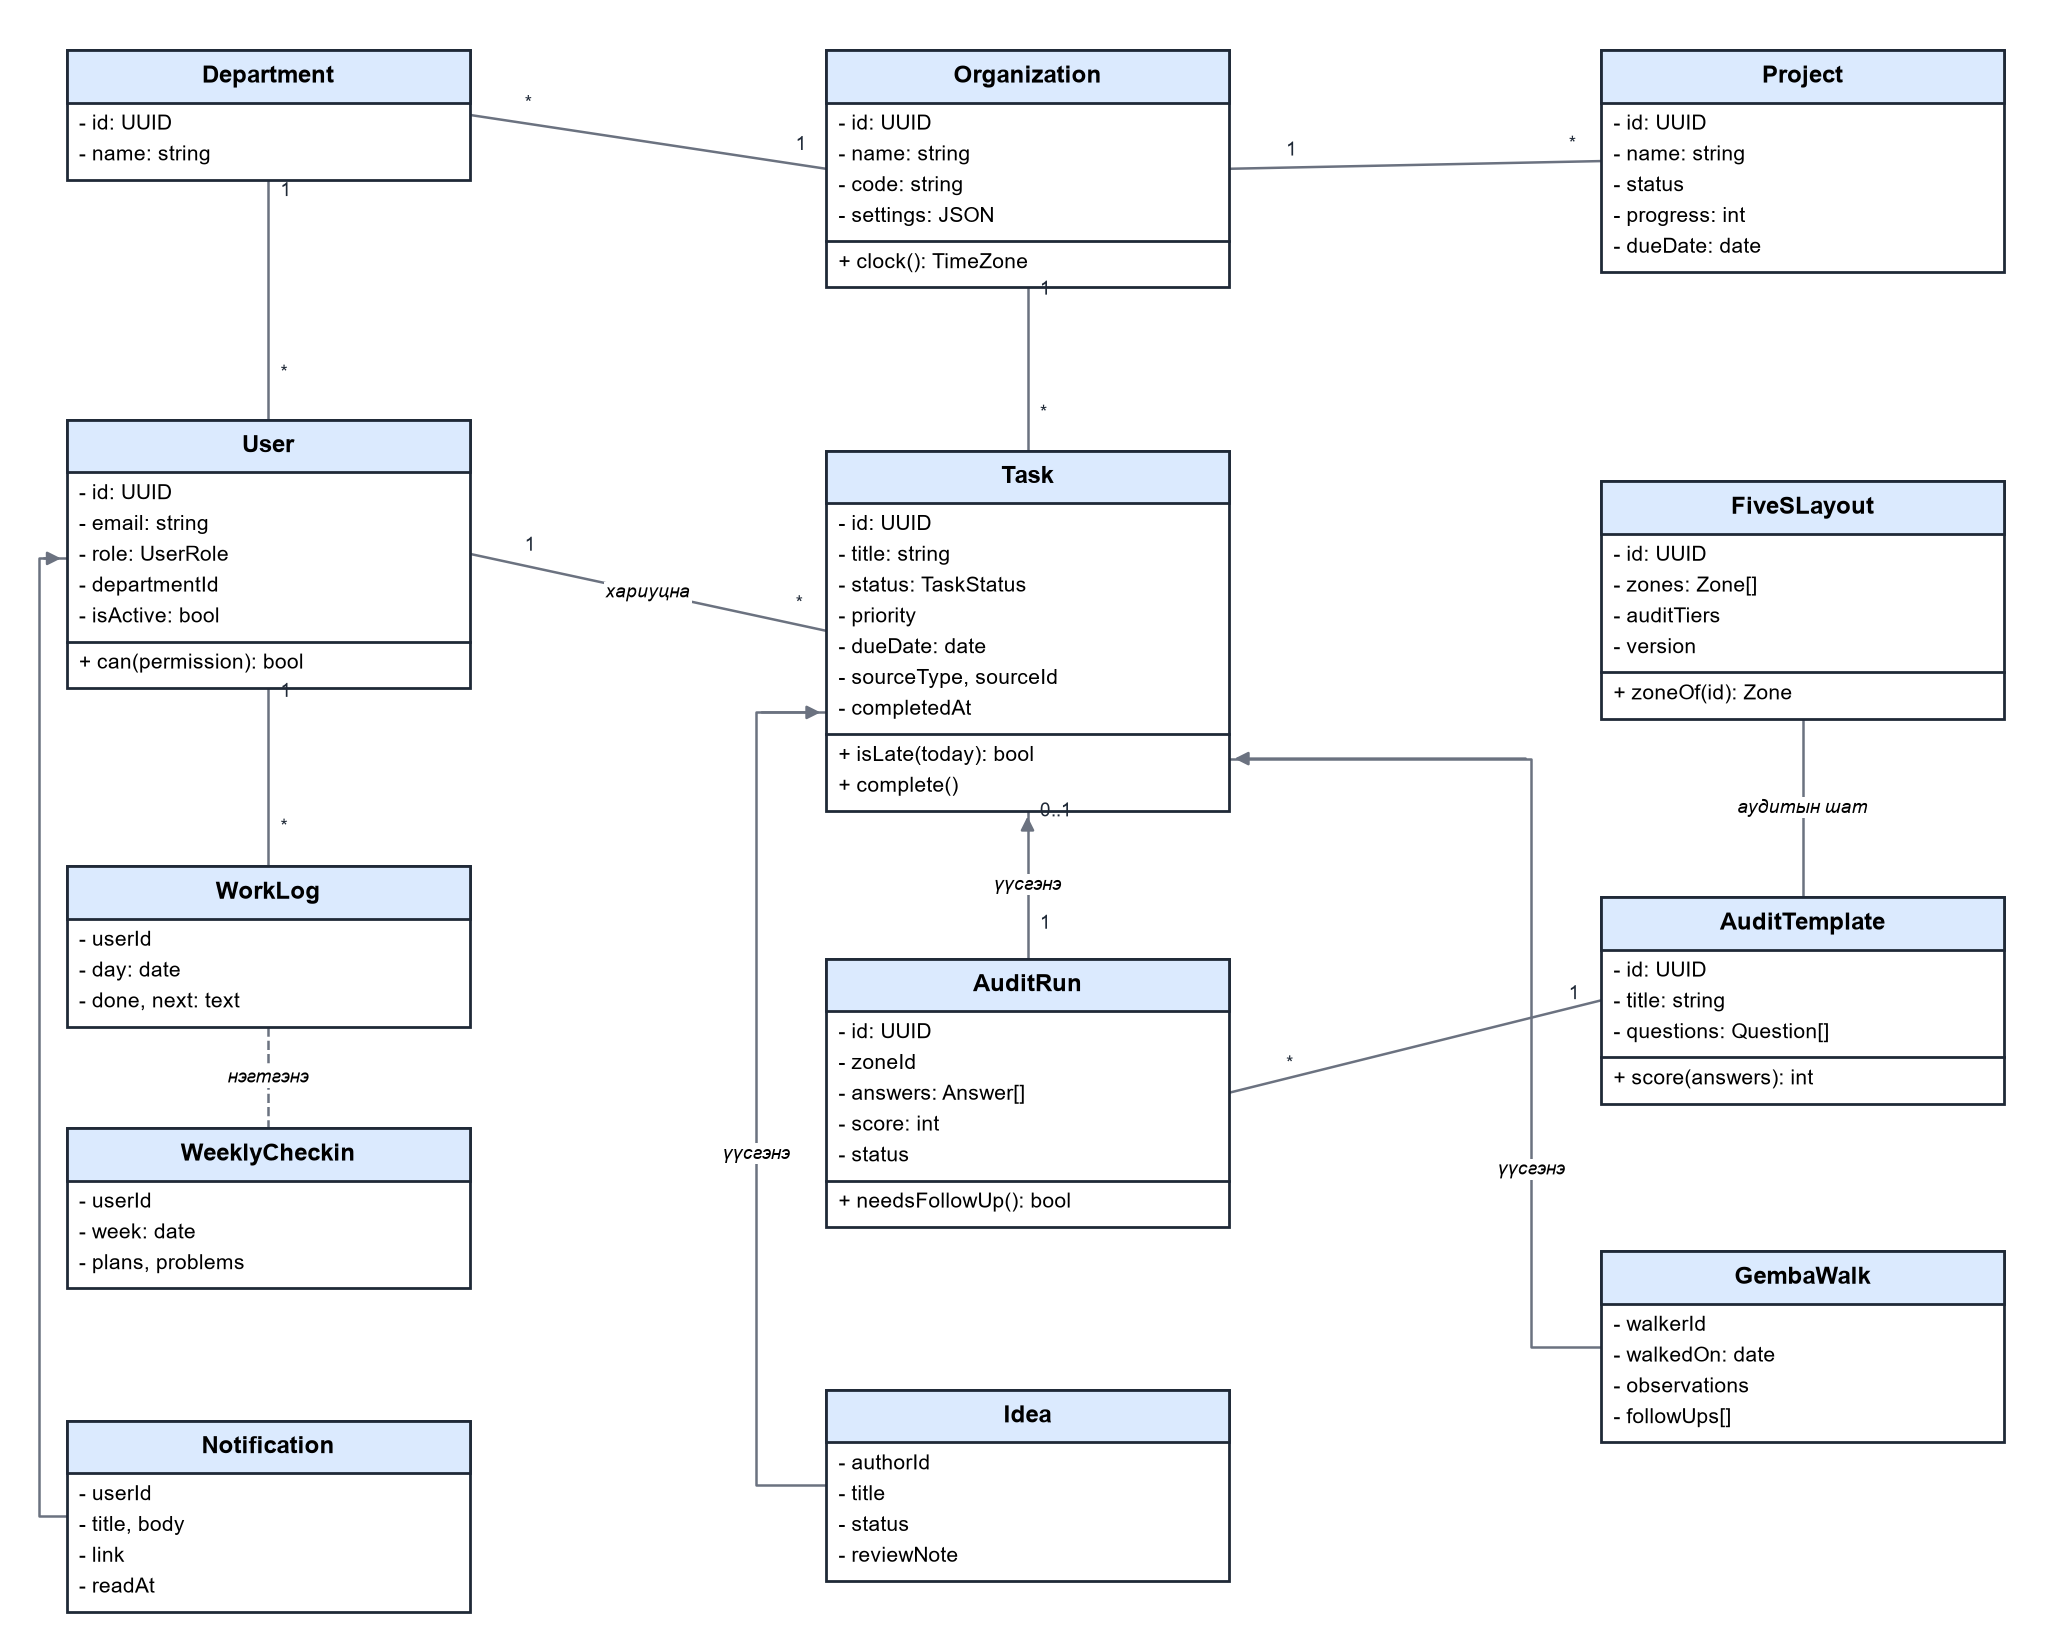
\includegraphics[width=\linewidth]{Figures/class_analysis.png}
\caption{Шинжилгээний класс диаграмм}
\label{fig:classA}
\end{figure}

%-------------------------------------------------------------------------------
\section{Шинжилгээний дарааллын диаграмм}
Зураг~\ref{fig:seqLogin}-д нэвтрэх, Зураг~\ref{fig:seqTask}-д ажил оноох үйл явцын объектуудын хоорондох мессежийн дарааллыг харуулав.

\begin{figure}[H]
\centering
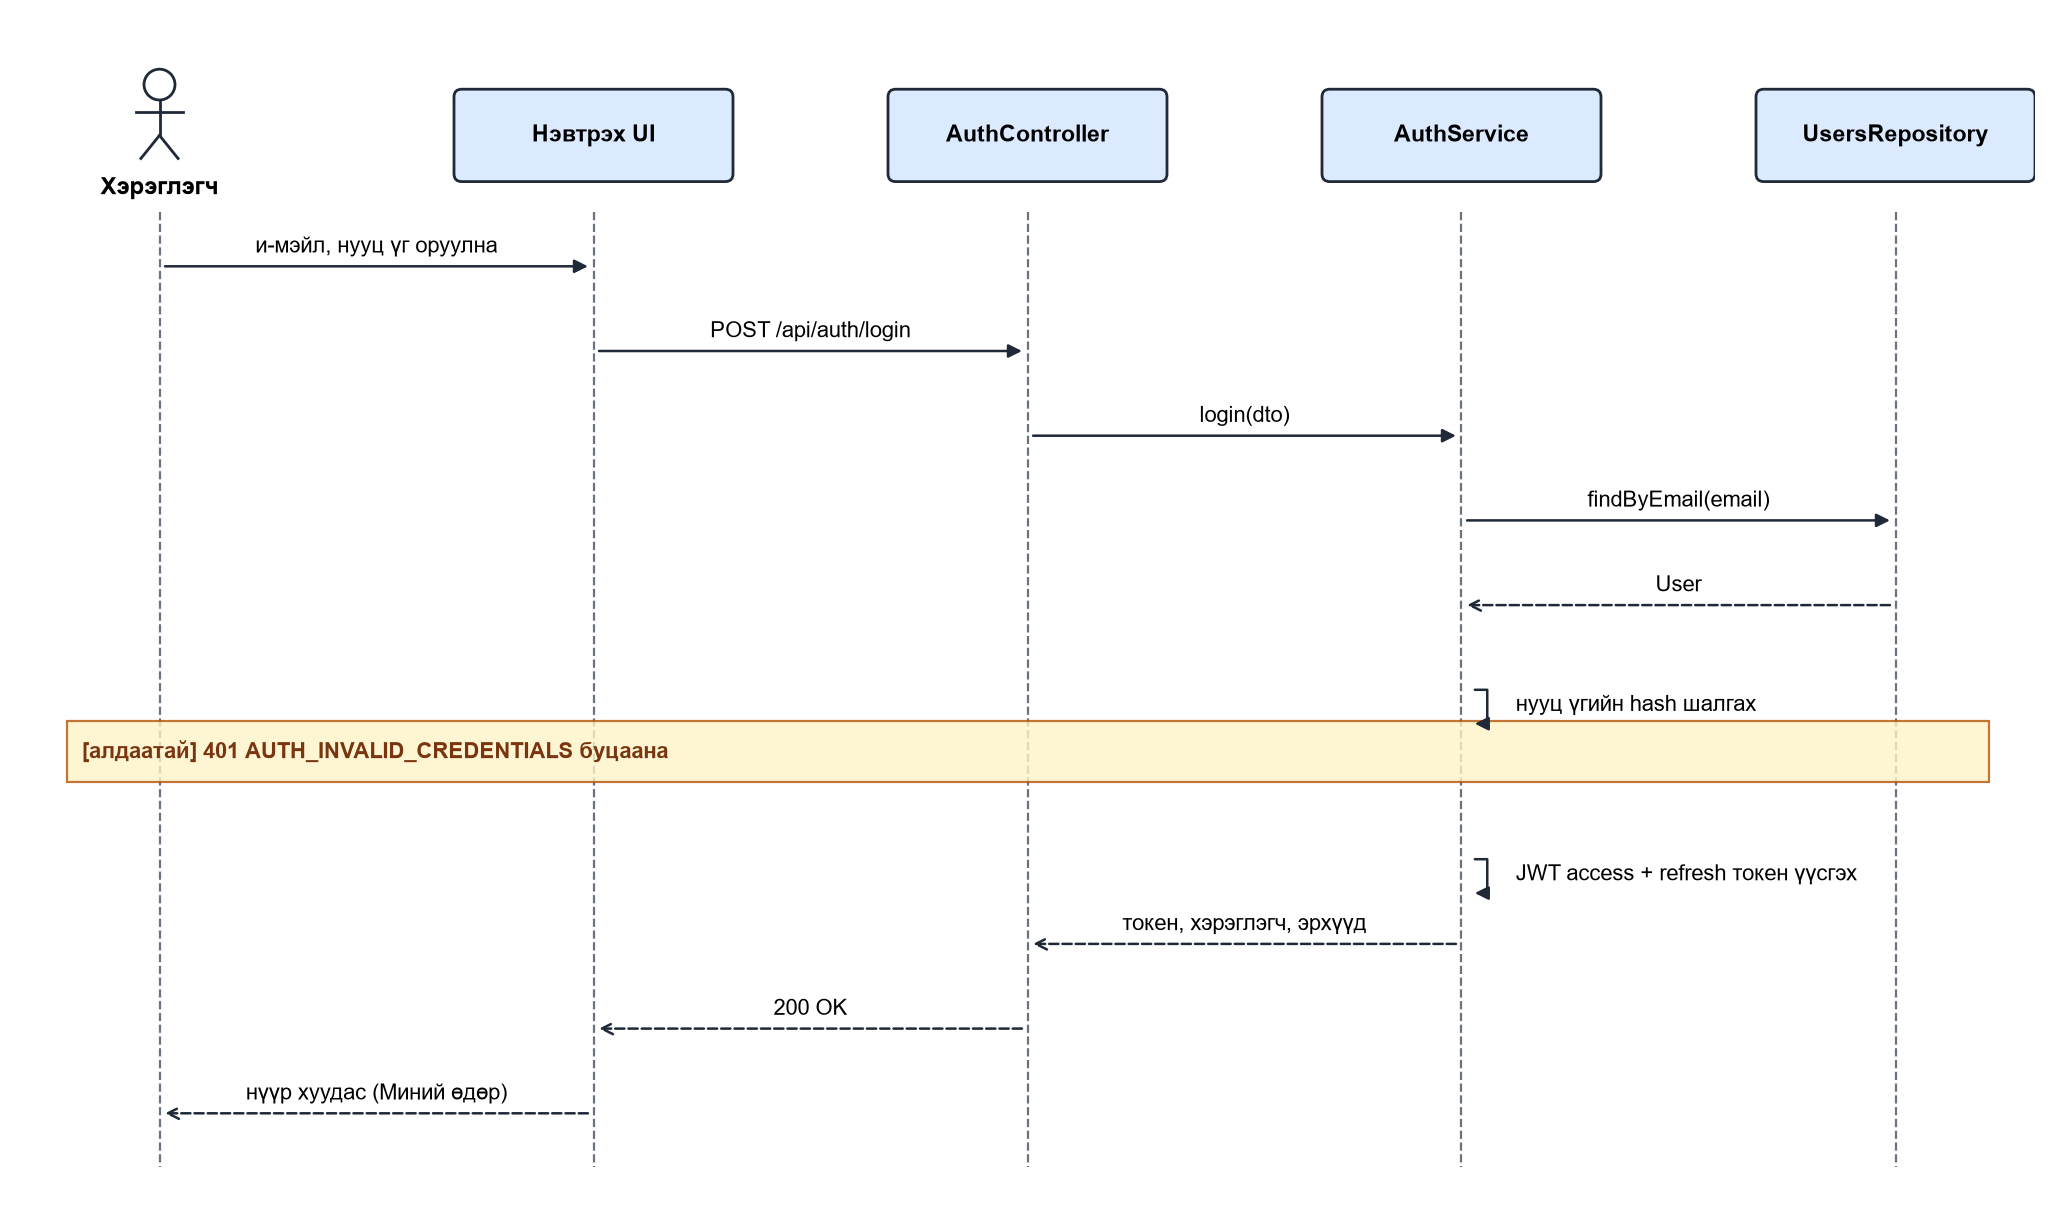
\includegraphics[width=\linewidth]{Figures/seq_login.png}
\caption{Нэвтрэх дарааллын диаграмм}
\label{fig:seqLogin}
\end{figure}

\begin{figure}[H]
\centering
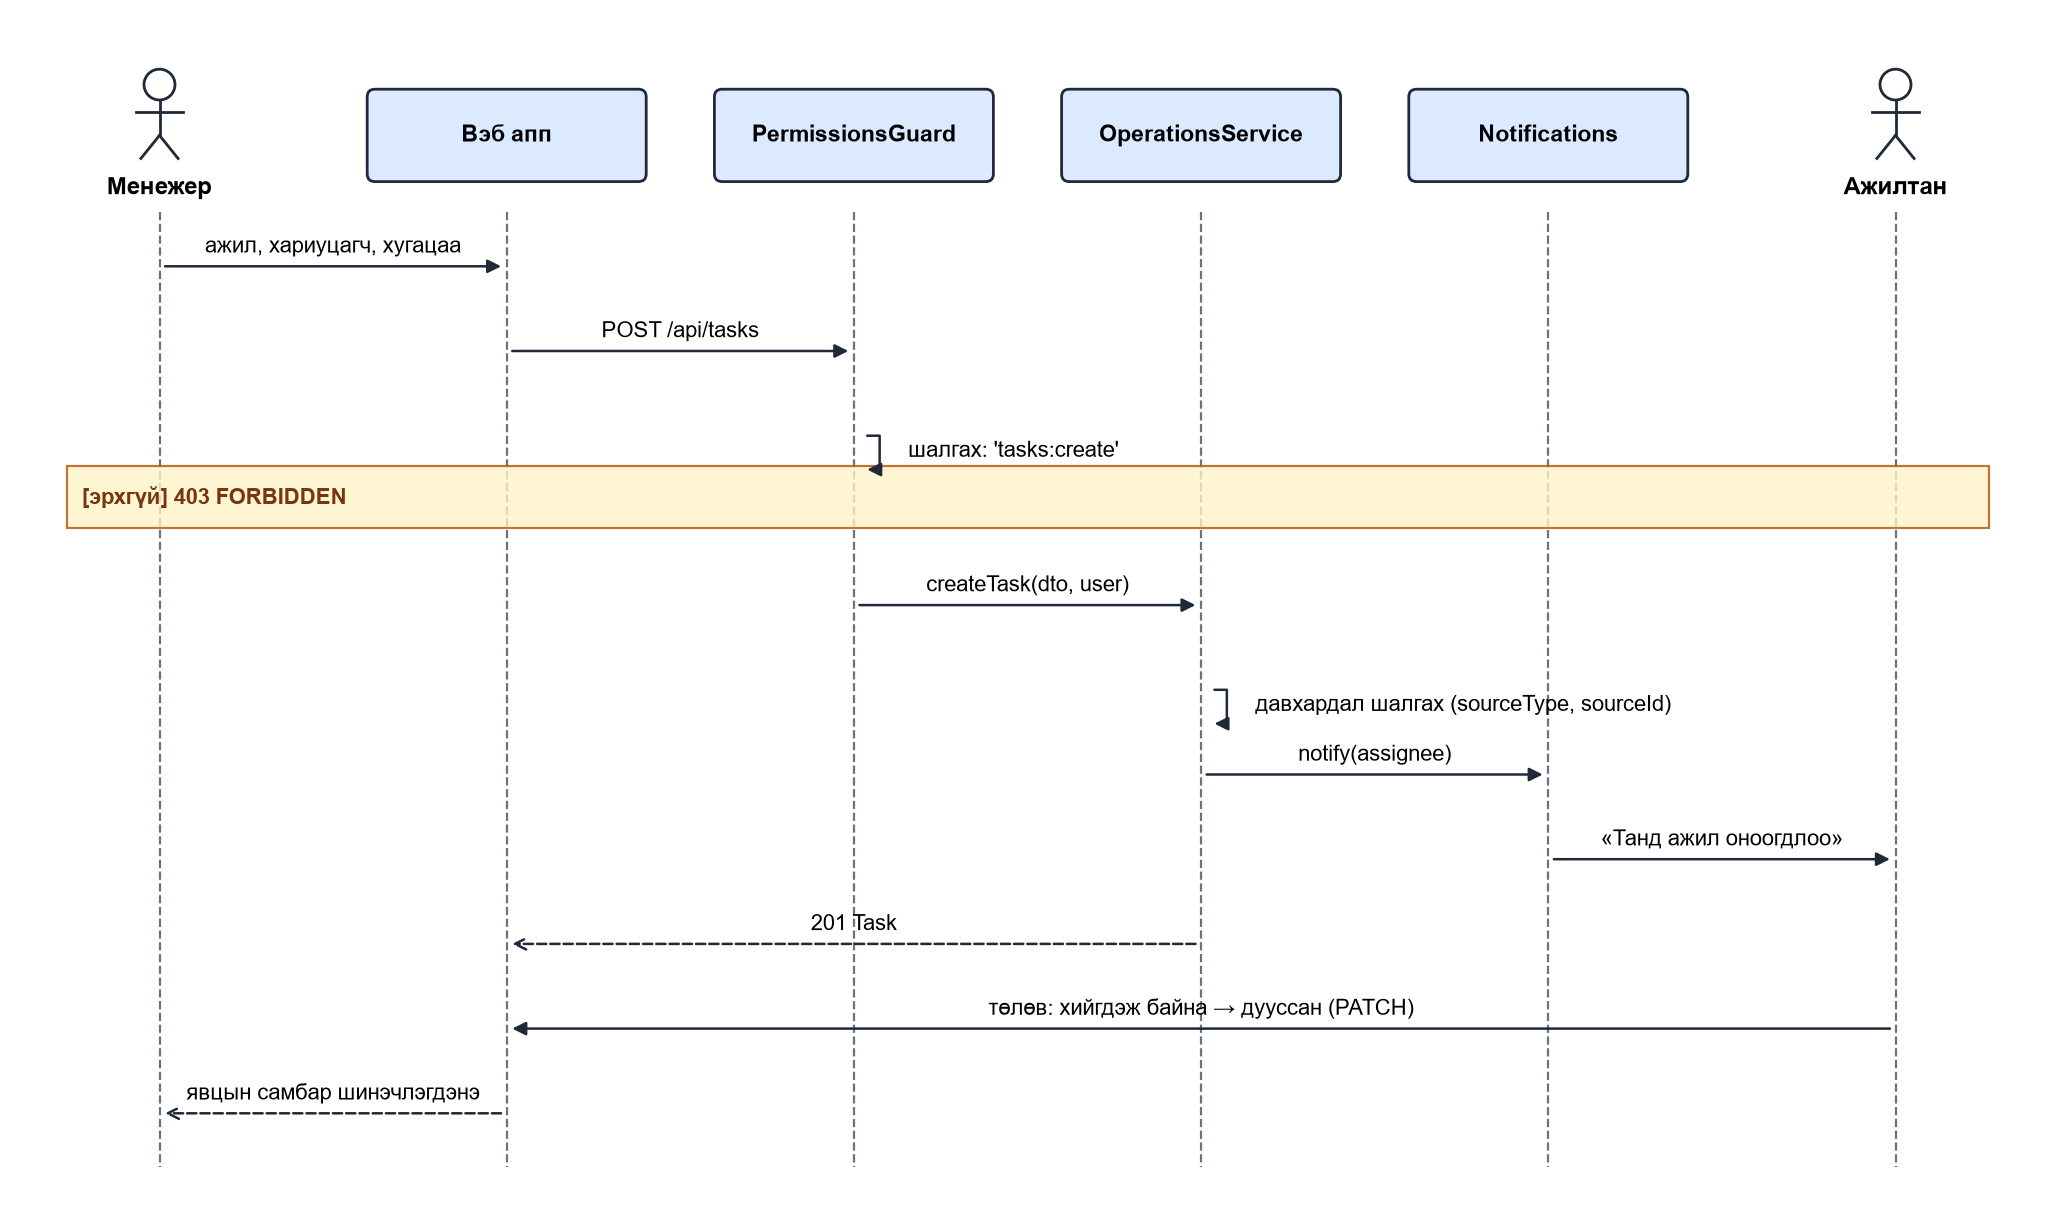
\includegraphics[width=\linewidth]{Figures/seq_task.png}
\caption{Ажил оноох дарааллын диаграмм}
\label{fig:seqTask}
\end{figure}

%-------------------------------------------------------------------------------
\section{Үйл ажиллагааны диаграмм}
Зураг~\ref{fig:activity}-д ажил оноогдохоос дуусах хүртэлх менежер, систем, ажилтны үйл ажиллагааг харуулав.

\begin{figure}[H]
\centering
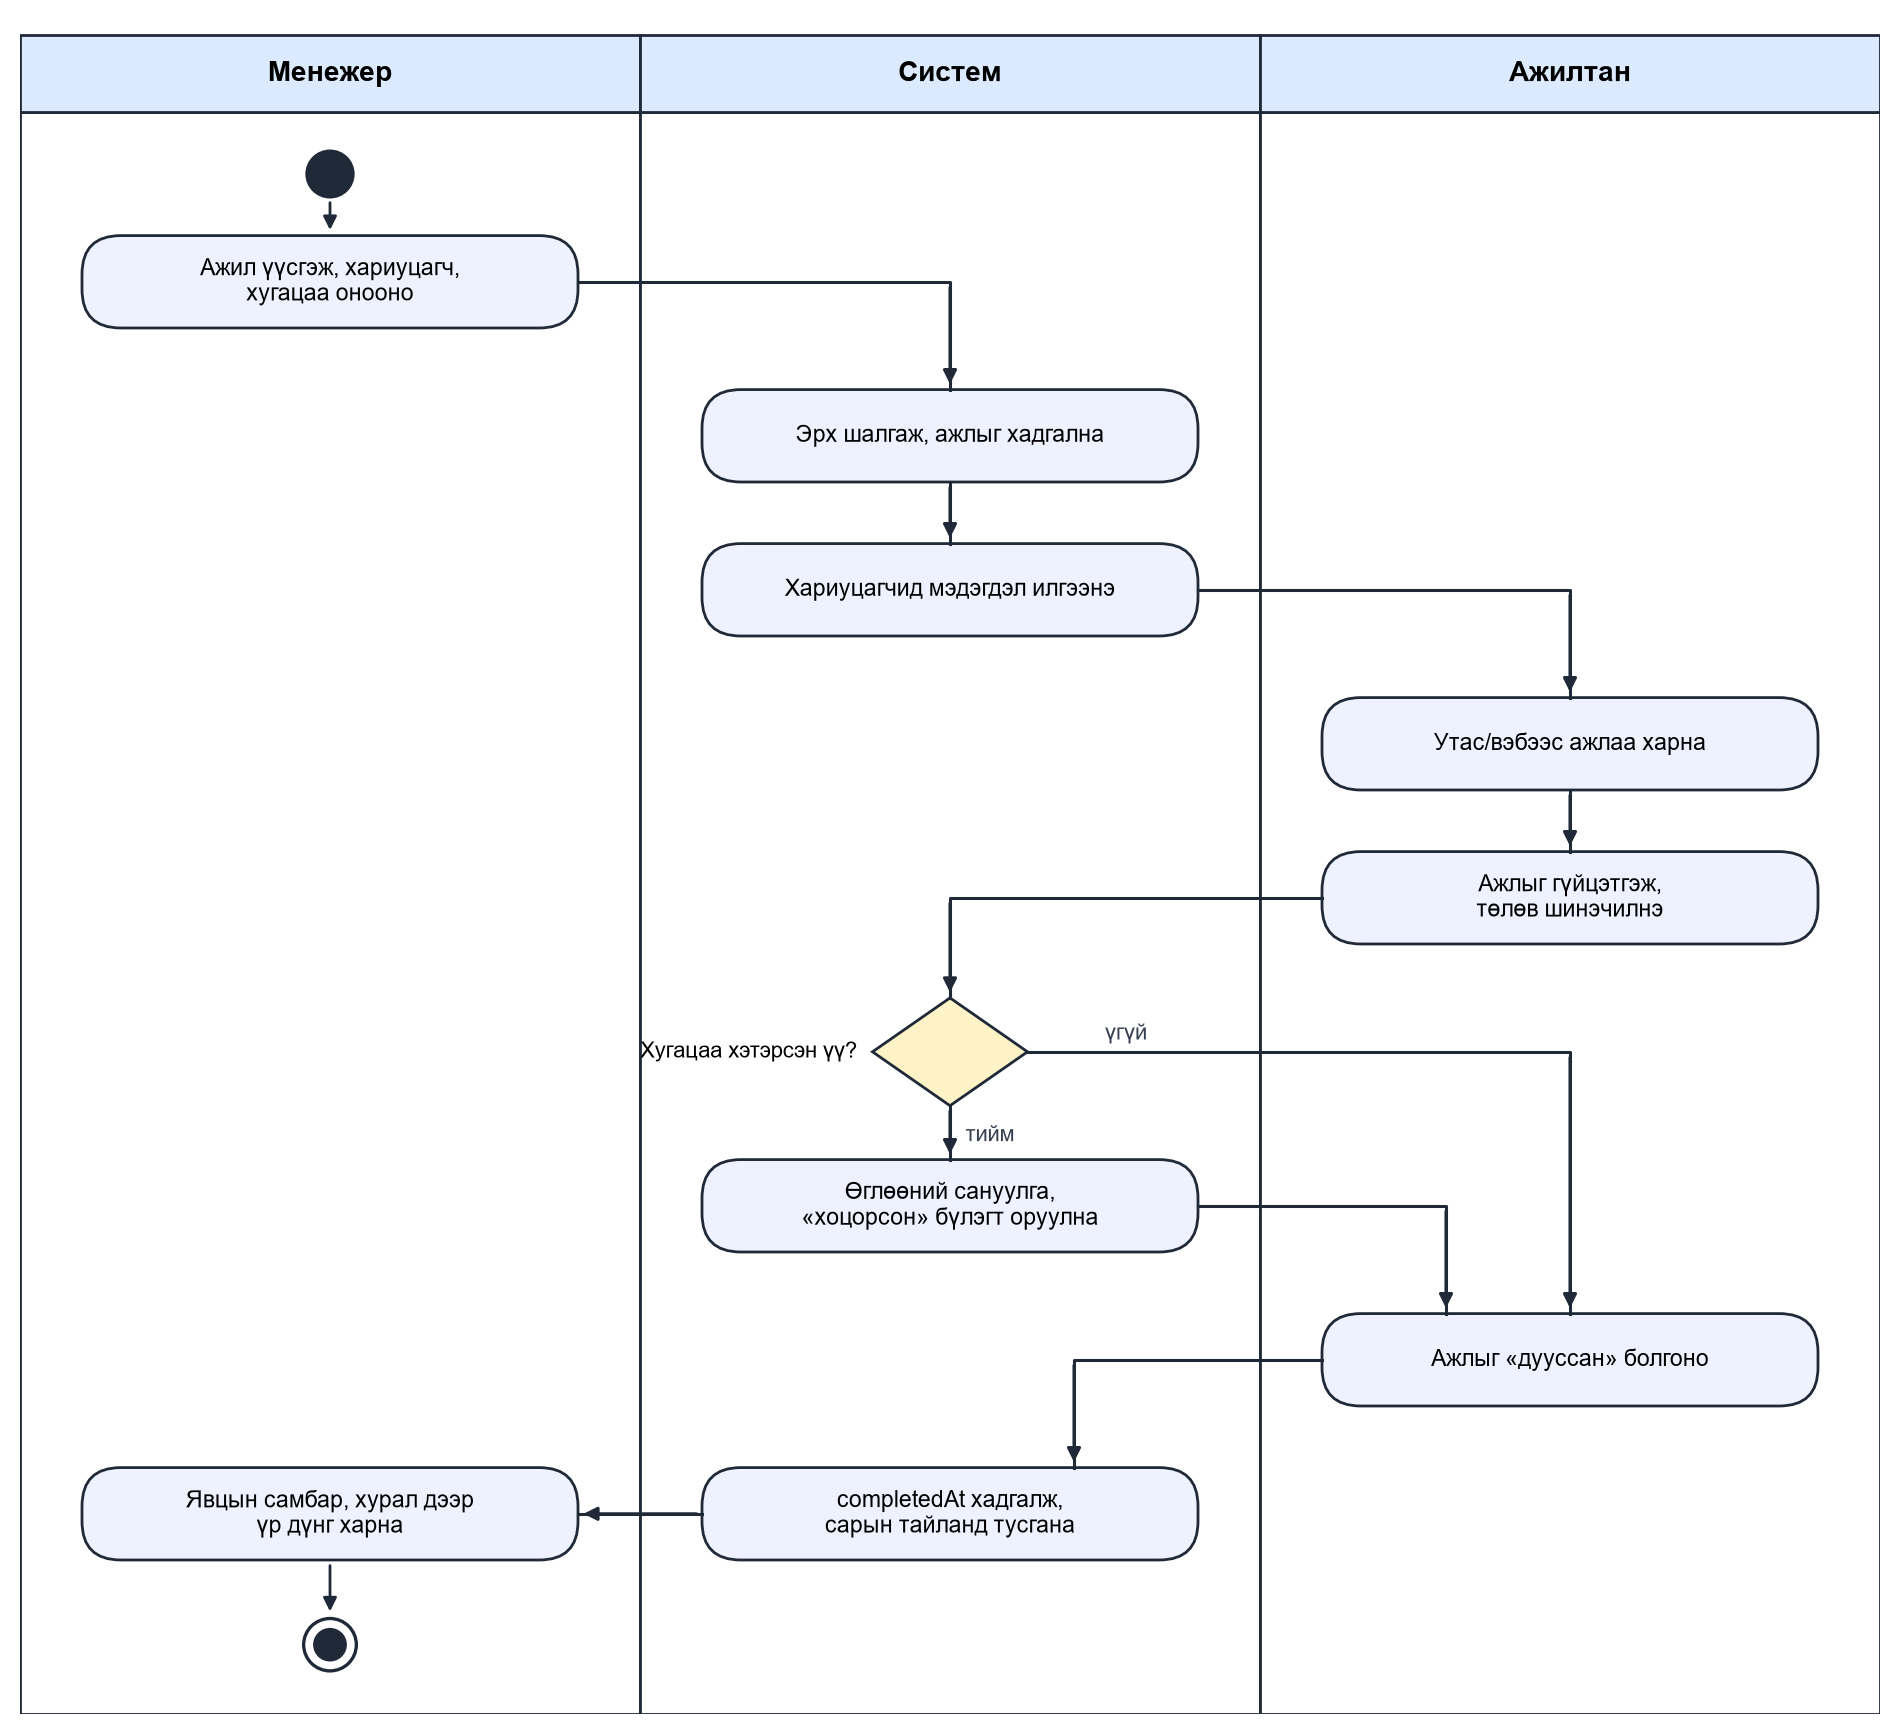
\includegraphics[width=0.9\linewidth]{Figures/activity_task.png}
\caption{Ажлын үйл ажиллагааны диаграмм}
\label{fig:activity}
\end{figure}

\section*{Бүлгийн дүгнэлт}
Энэ бүлэгт системийн үйл ажиллагааг хэрэглэгчийн дүрээр тодорхойлж, 22 функциональ, 10 функциональ бус шаардлага боловсруулав. Use-case диаграмм, есөн use-case-ийн дэлгэрэнгүй тодорхойлолт, шаардлагын мөрдөх матриц, шинжилгээний класс, дараалал, үйл ажиллагааны диаграммаар системийн зан төлөвийг загварчлав.

% Бүлэг 3

\chapter{Системийн зохиомж}
\label{Chapter3}

%-------------------------------------------------------------------------------
\section{Системийн архитектурын зураглал}
Систем нь клиент--сервер загварт суурилсан, гурван үндсэн хэсгээс бүрдэнэ (Зураг~\ref{fig:arch}): вэб апп, гар утасны апп ба нэгдсэн backend API. Хоёр клиент ижил REST API-г HTTPS/JSON-оор ашигладаг тул бизнесийн дүрэм нэг газар (сервер дээр) хэрэгжиж, клиентүүдийн хооронд зөрөхгүй~\cite{fowler,martin}.

\begin{figure}[H]
\centering
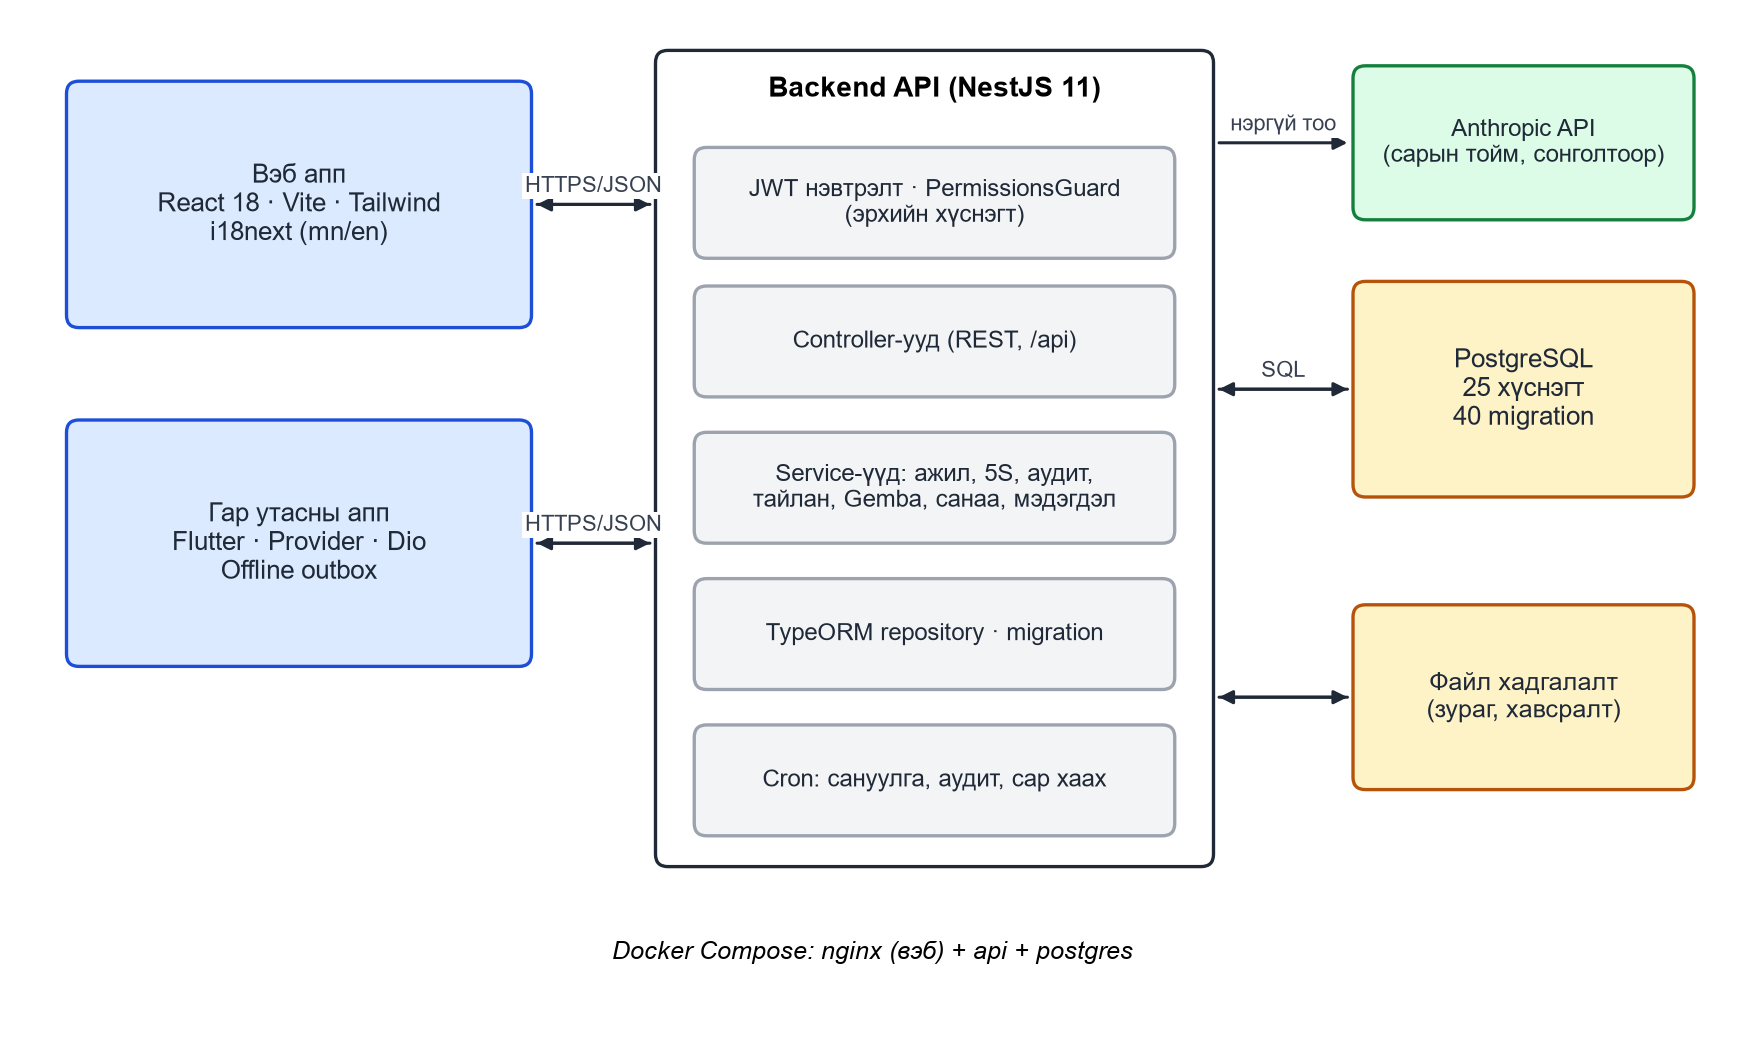
\includegraphics[width=\linewidth]{Figures/architecture.png}
\caption{Системийн архитектур}
\label{fig:arch}
\end{figure}

Backend нь давхаргат бүтэцтэй:
\begin{itemize}
    \item \textbf{Хамгаалалтын давхарга} -- JWT токеныг шалгаж, PermissionsGuard нь маршрут бүрийн шаардсан эрхийг хэрэглэгчийн дүрийн эрхийн хүснэгттэй тулгана. Вэбийн товчлуурыг харуулах эсэх ч мөн энэ хүснэгтээс шийдэгддэг тул клиент, сервер хоёр зөрөхгүй.
    \item \textbf{Controller давхарга} -- HTTP хүсэлтийг хүлээн авч, DTO-оор оролтыг шалгана.
    \item \textbf{Service давхарга} -- бизнесийн дүрэм: ажил, 5S, аудит, тайлан, Gemba, санаа, мэдэгдэл.
    \item \textbf{Өгөгдлийн давхарга} -- TypeORM repository; схемийн өөрчлөлт бүр migration файлаар хийгдэнэ.
    \item \textbf{Цагийн хуваарьт үйлдэл} -- өглөөний сануулга, аудитын хуваарь, сар хаах.
\end{itemize}

%-------------------------------------------------------------------------------
\section{Байршуулалтын диаграмм}
Систем Docker Compose-оор нэг Linux серверт байршина (Зураг~\ref{fig:deploy}). admin-web контейнер (nginx) вэб аппын статик файлыг түгээж, \texttt{/api} хүсэлтийг backend рүү дамжуулна; гар утасны апп API-д HTTPS-ээр шууд хандана. Өгөгдлийн сан болон хавсралт файлууд тусдаа volume-д хадгалагдах тул контейнерийг шинэчлэхэд өгөгдөл алдагдахгүй. Нөөц хуулбар (backup), хяналт (prometheus, grafana), кэш (redis) нь шаардлагатай үед идэвхжүүлэх сонголттой үйлчилгээ юм. Өгөгдлийн сангийн нөөцөөс гадна хавсралтын volume-г тусад нь нөөцлөх шаардлагатай.

\begin{figure}[H]
\centering
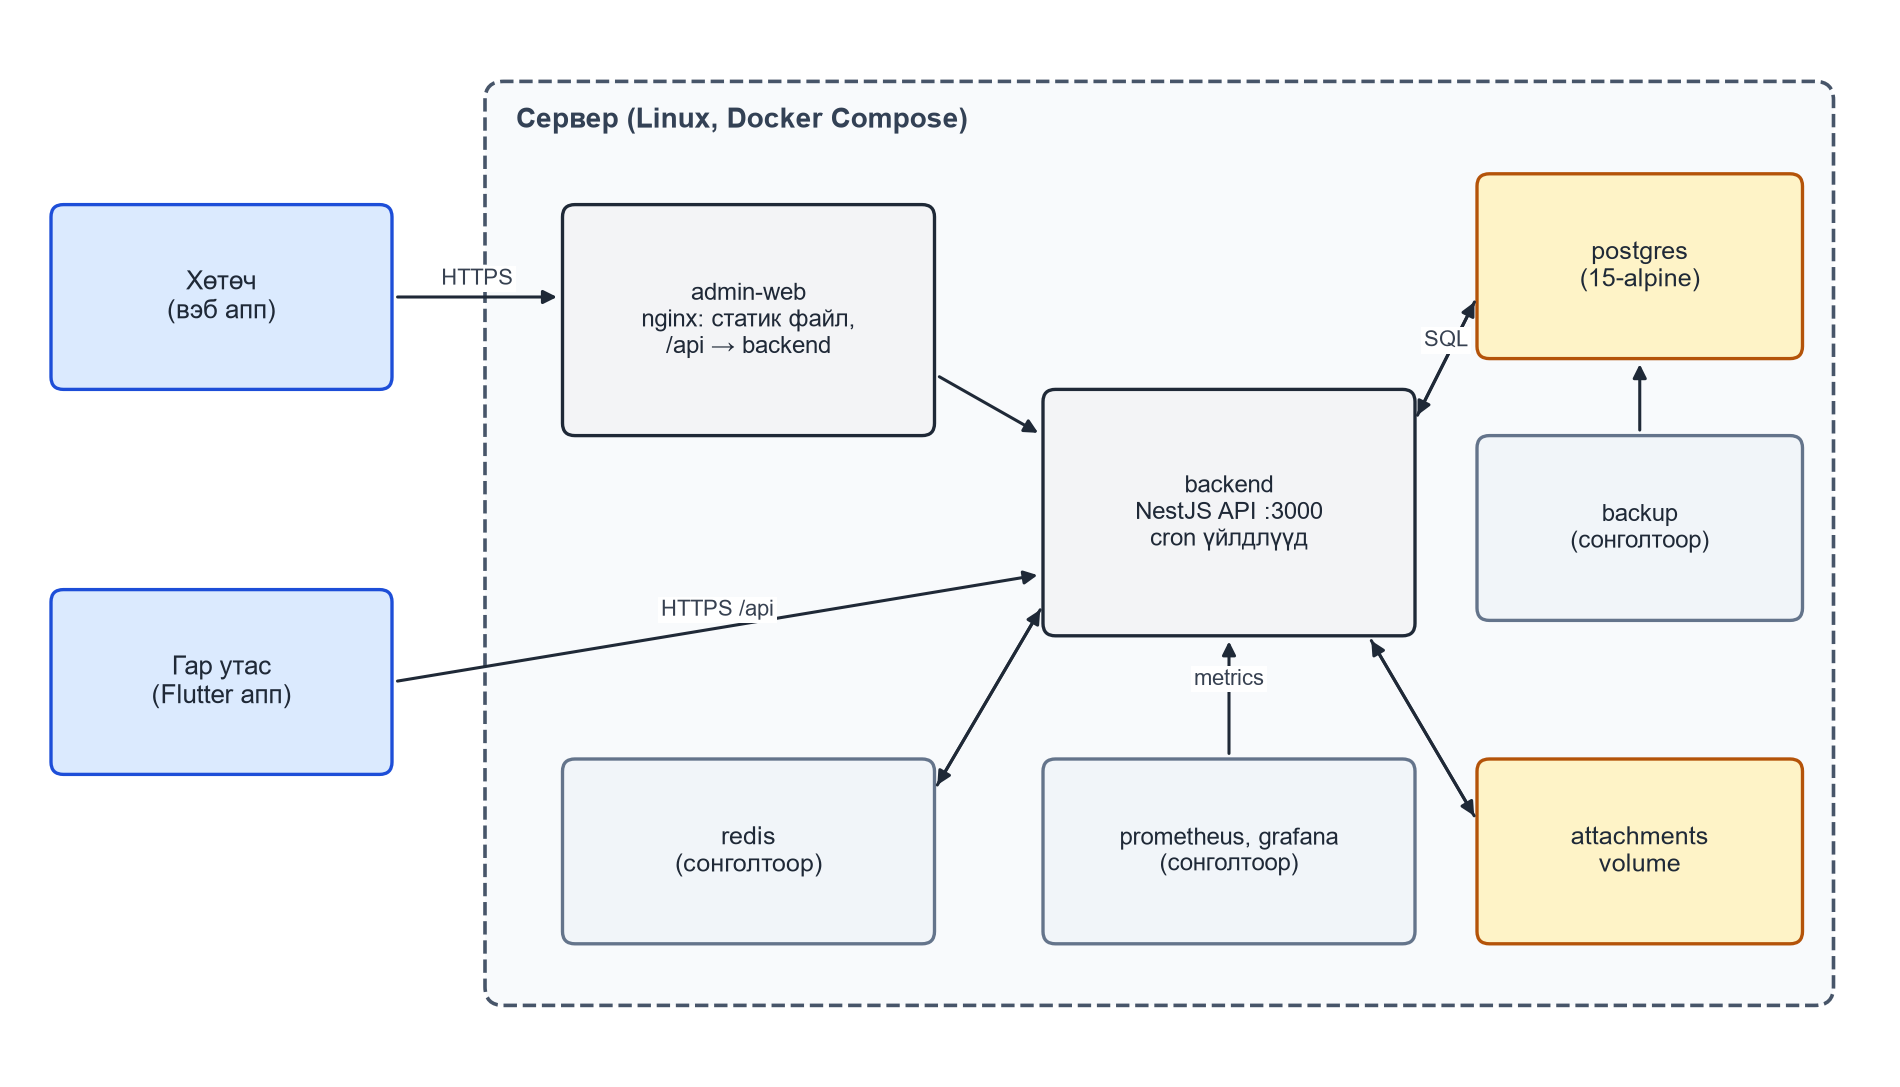
\includegraphics[width=\linewidth]{Figures/deployment.png}
\caption{Байршуулалтын диаграмм}
\label{fig:deploy}
\end{figure}

%-------------------------------------------------------------------------------
\section{Зохиомжийн шатны класс диаграмм}
Зураг~\ref{fig:classD}-д backend-ийн гол классууд ба тэдгээрийн хамаарлыг харуулав. Controller нь guard-аар хамгаалагдаж, service-ийг дуудна; service нь repository-оор дамжин өгөгдлийн сантай ажиллаж, мэдэгдлийн service-ээр хэрэглэгчид мэдэгдэнэ.

\begin{figure}[H]
\centering
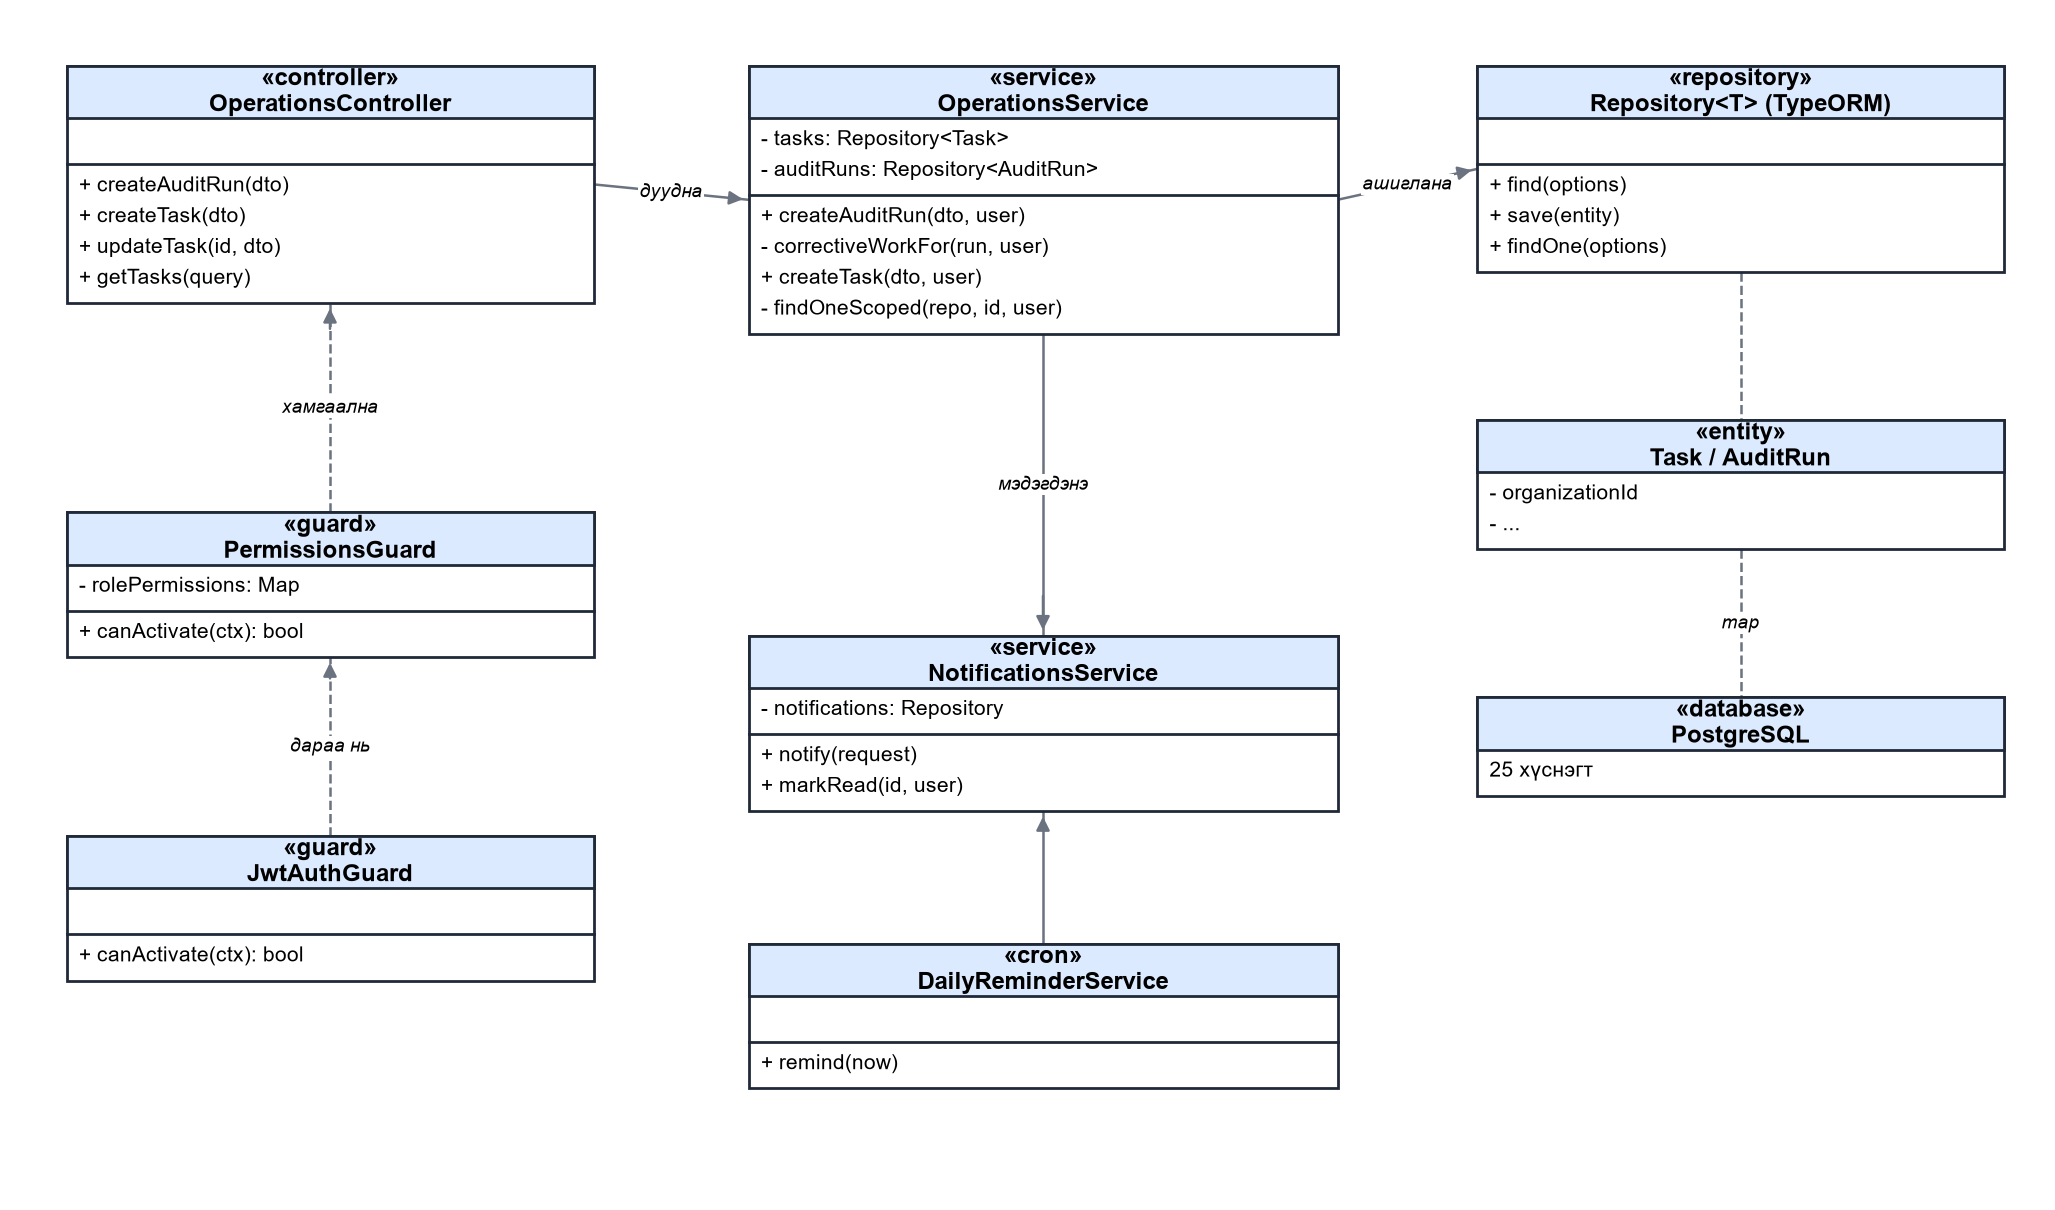
\includegraphics[width=\linewidth]{Figures/class_design.png}
\caption{Зохиомжийн класс диаграмм}
\label{fig:classD}
\end{figure}

%-------------------------------------------------------------------------------
\section{Зохиомжийн шатны дарааллын диаграмм}
Зураг~\ref{fig:seqAudit}-д гар утаснаас 5S аудит хийх, оноо босгоос доош бол засах ажил үүсгэх үйл явцыг харуулав.

\begin{figure}[H]
\centering
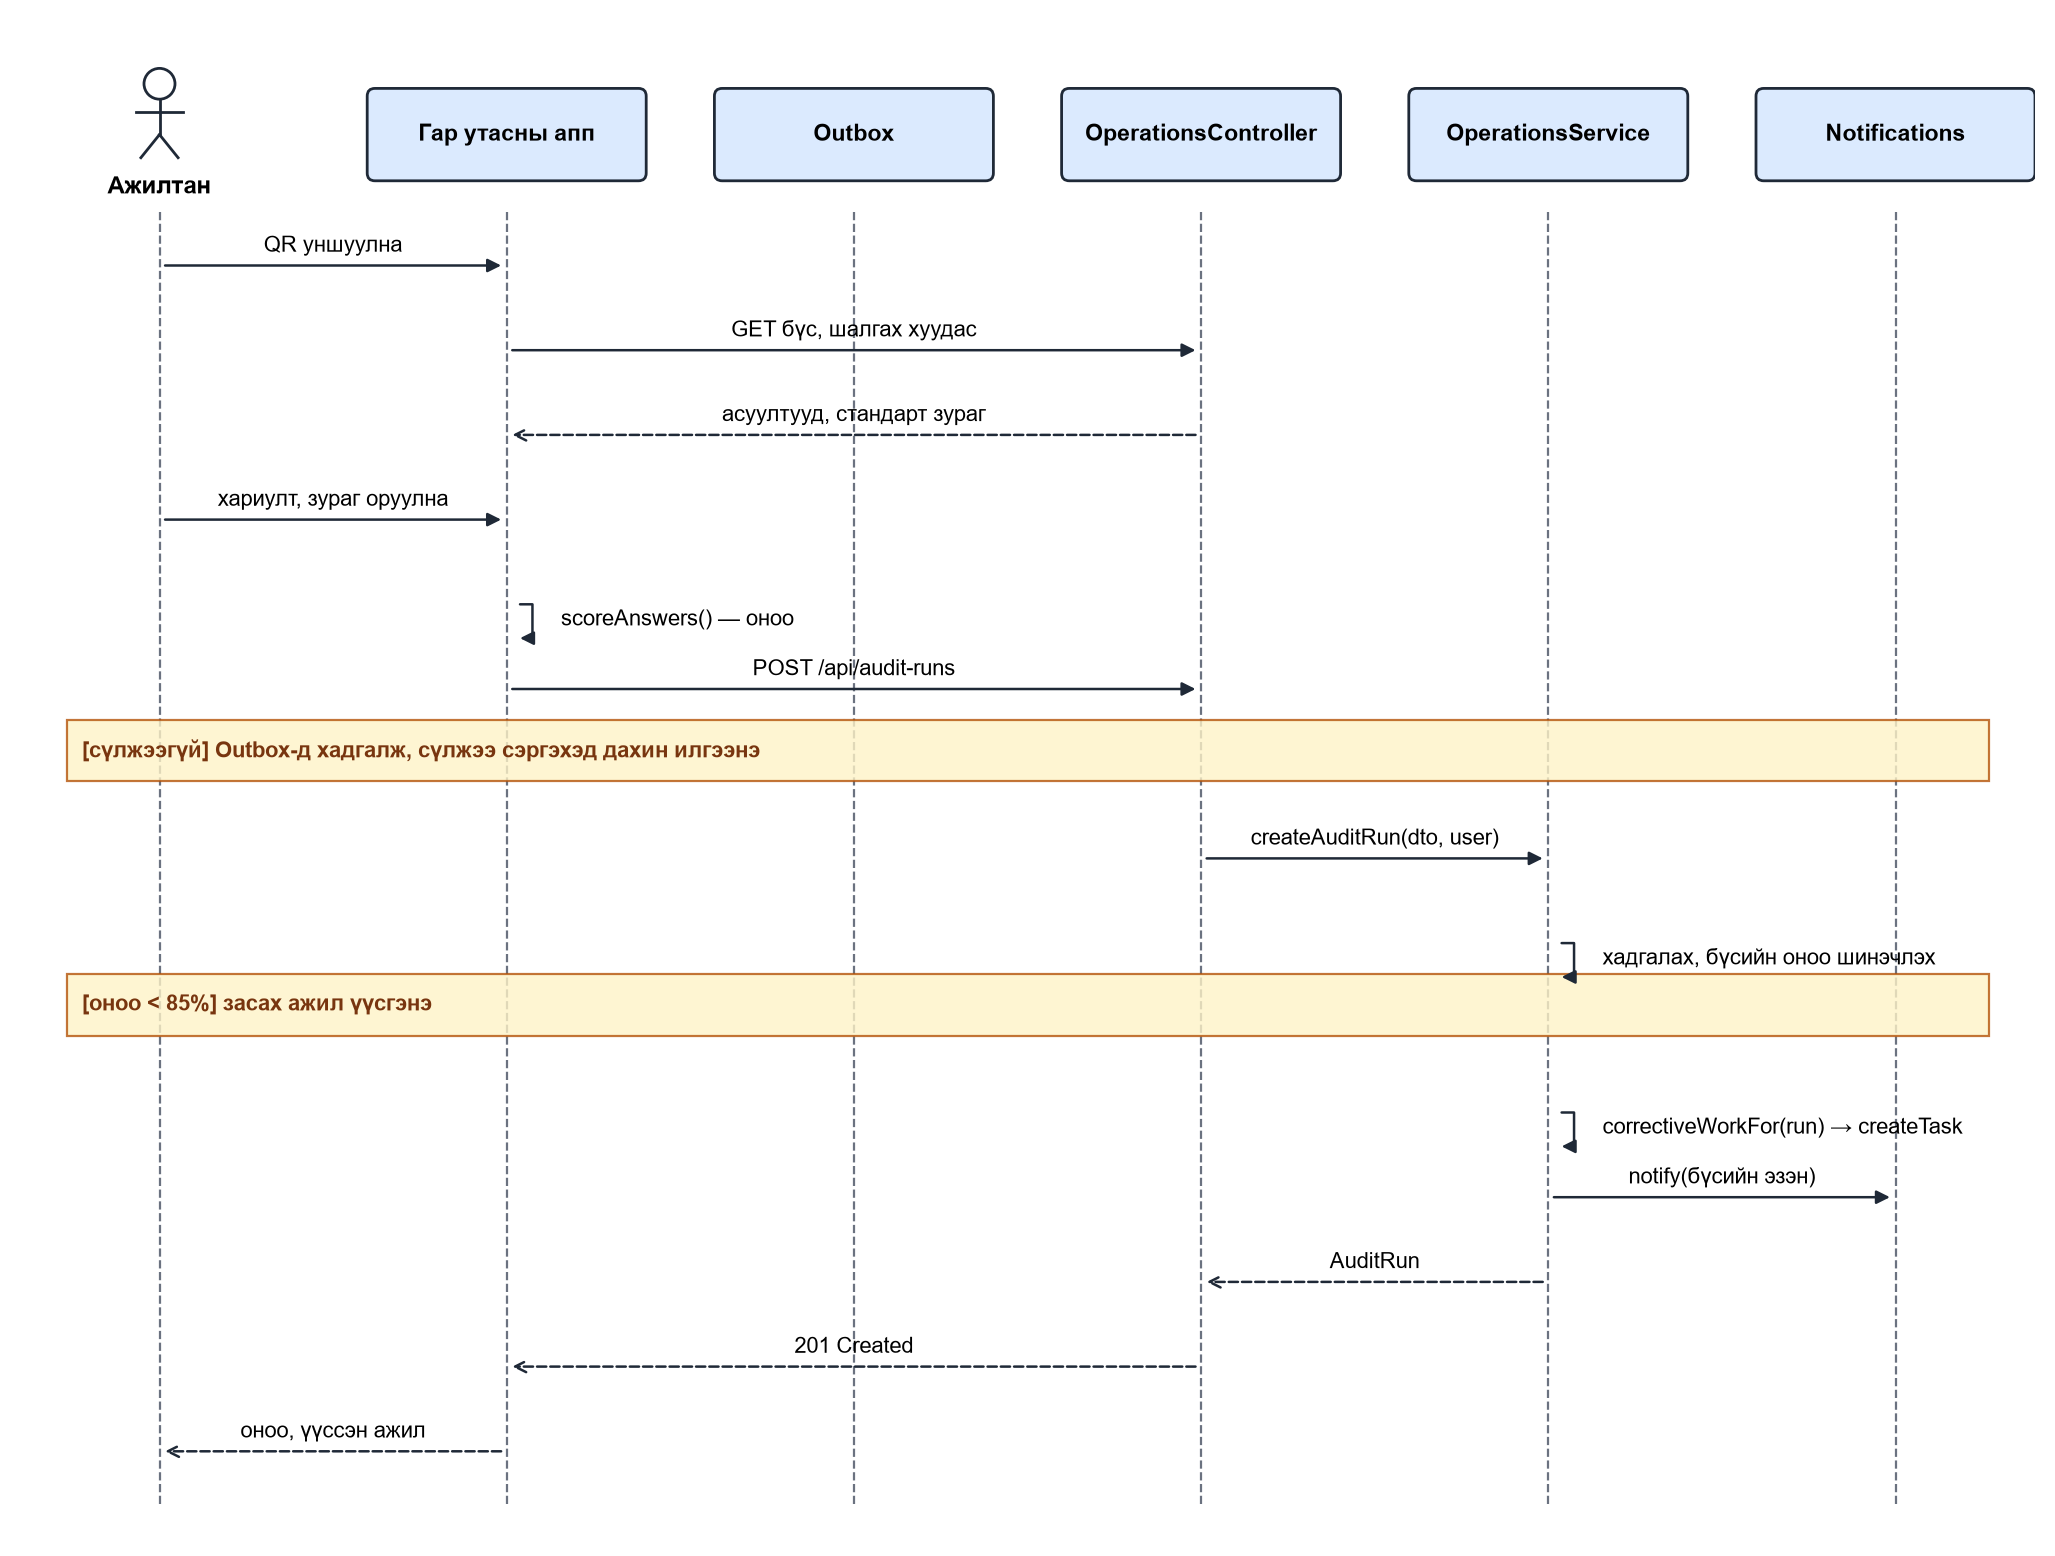
\includegraphics[width=\linewidth]{Figures/seq_audit.png}
\caption{5S аудит хийх зохиомжийн дарааллын диаграмм}
\label{fig:seqAudit}
\end{figure}

Зураг~\ref{fig:seqClose}-д сарын тайланг автоматаар хаах, Зураг~\ref{fig:seqGemba}-д Gemba явалт бүртгэж дараагийн алхмуудыг ажил болгох үйл явцыг харуулав.

\begin{figure}[H]
\centering
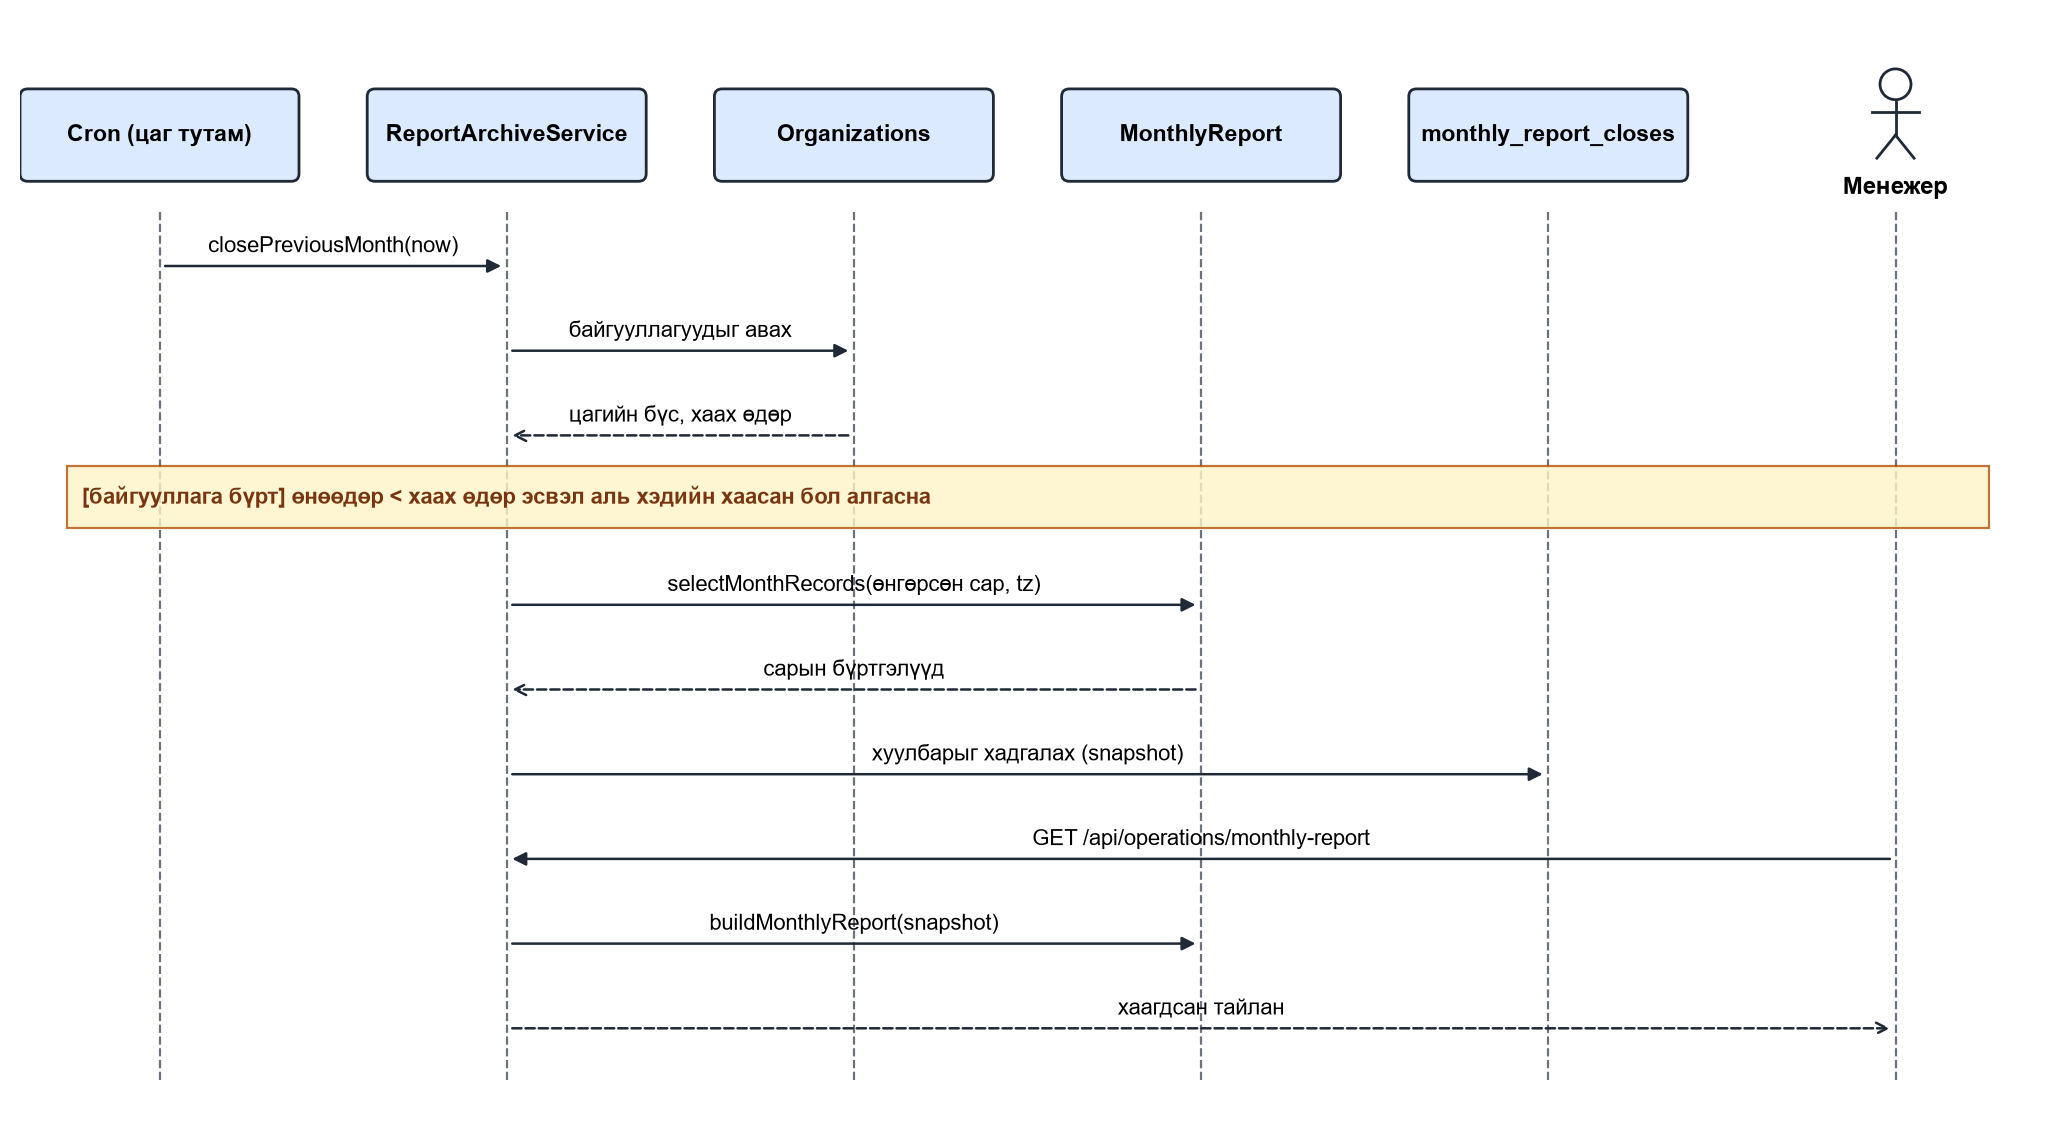
\includegraphics[width=\linewidth]{Figures/seq_close.png}
\caption{Сарын тайлан хаах зохиомжийн дарааллын диаграмм}
\label{fig:seqClose}
\end{figure}

\begin{figure}[H]
\centering
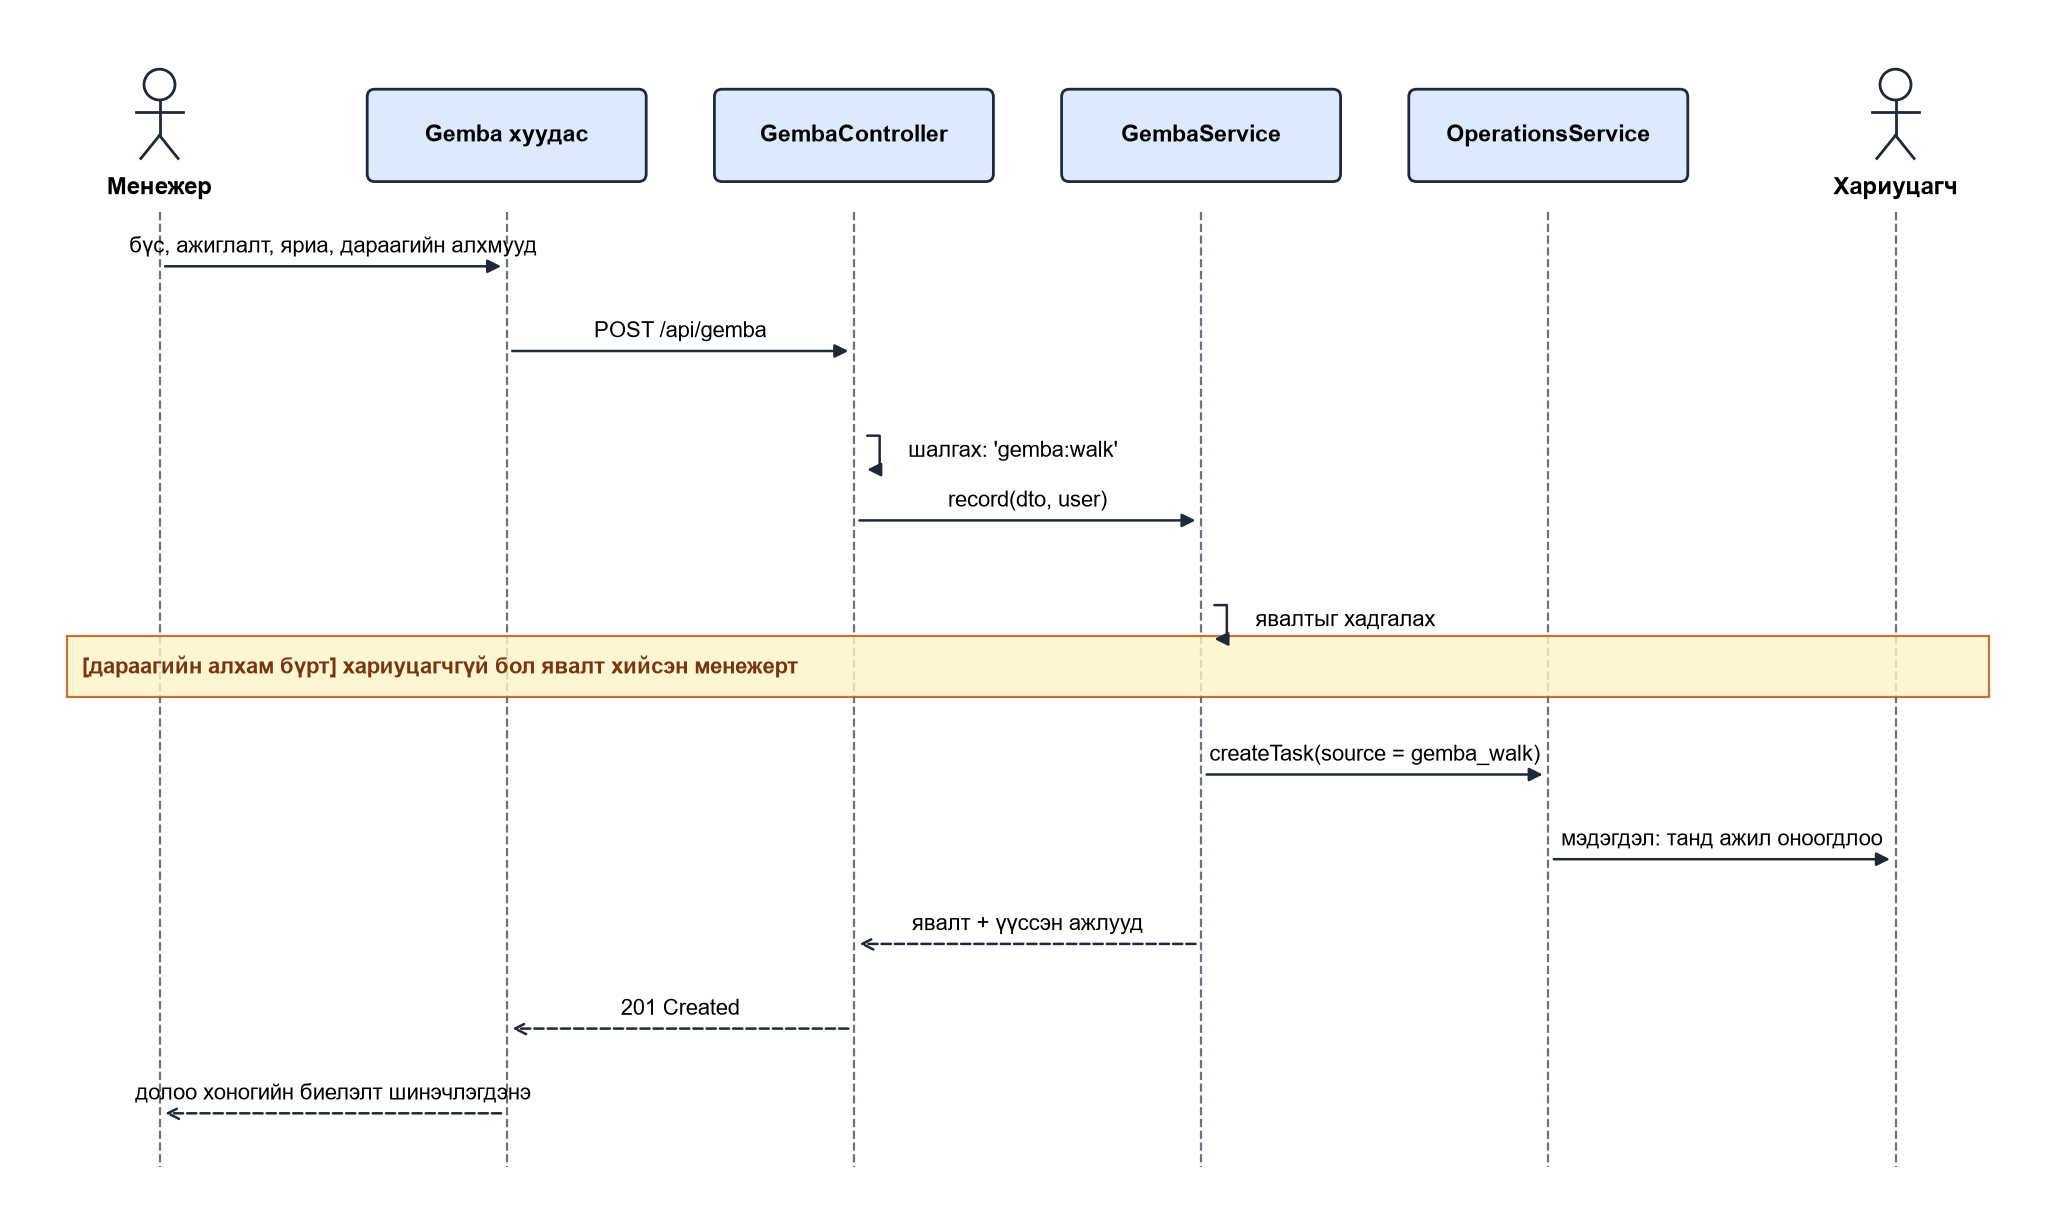
\includegraphics[width=\linewidth]{Figures/seq_gemba.png}
\caption{Gemba явалт бүртгэх зохиомжийн дарааллын диаграмм}
\label{fig:seqGemba}
\end{figure}

%-------------------------------------------------------------------------------
\section{Өгөгдлийн сангийн ерөнхий схем}
Өгөгдлийн сан 25 хүснэгтээс бүрдэх бөгөөд одоогийн схемийг 38 runtime/operations migration-оор байгуулна. Бүх хүснэгт organizationId-аар байгууллагад харьяалагдаж, хүсэлт бүр хэрэглэгчийн байгууллагаар шүүгдэнэ. Зураг~\ref{fig:erd}-д гол хүснэгтүүд ба холбоосыг харуулав.

\begin{figure}[H]
\centering
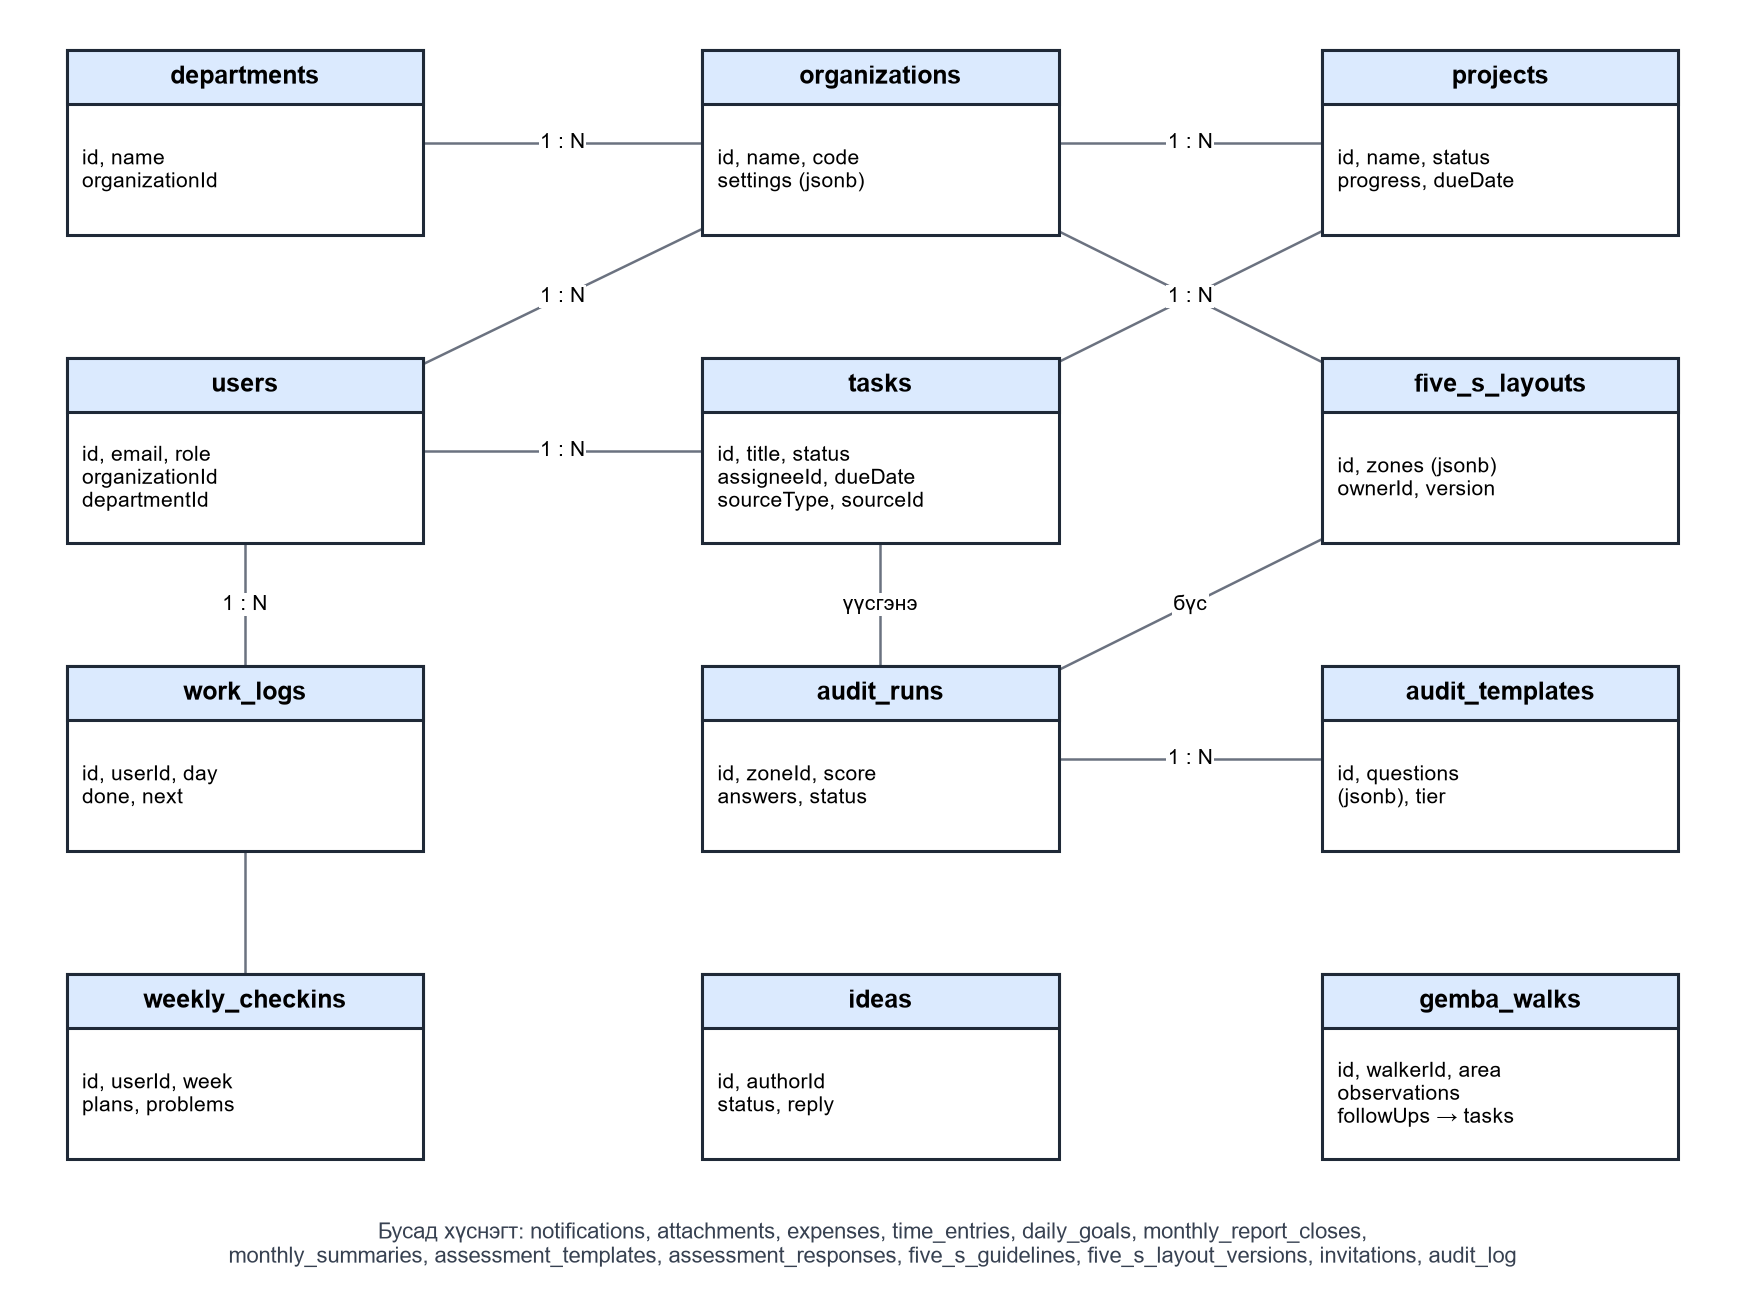
\includegraphics[width=\linewidth]{Figures/er.png}
\caption{Өгөгдлийн сангийн ерөнхий схем}
\label{fig:erd}
\end{figure}

\begin{itemize}
    \item \textbf{tasks} хүснэгт sourceType, sourceId талбараар ажил хаанаас үүссэнийг (аудит, Gemba, санаа, гараар) хадгална. Ингэснээр нэг эх сурвалжаас ажил давхар үүсэхээс сэргийлж, тайланд гарал үүслээр ангилна.
    \item \textbf{five\_s\_layouts} хүснэгт талбайн бүсүүдийг JSONB хэлбэрээр хадгалж, өөрчлөлт бүрийг five\_s\_layout\_versions-д архивлана.
    \item \textbf{monthly\_report\_closes} хүснэгт хаагдсан сарын бүртгэлүүдийн хуулбарыг хадгалж, дараа нь өгөгдөл өөрчлөгдсөн ч тайлан тогтвортой үлдэнэ.
\end{itemize}

%-------------------------------------------------------------------------------
\section{Эрхийн загвар}
Эрхийг дүрд суурилсан хандалтын хяналт (RBAC) аргаар зохион байгуулав. Эрх нь ``нөөц:үйлдэл'' хэлбэртэй (жишээ нь tasks:create, reports:close). Дүр бүрийн эрхийн жагсаалт доод дүрийн жагсаалтыг бүрэн агуулж байхаар хуримтлуулан бичигдсэн тул ``менежер ажилтны бүх эрхтэй'' гэсэн шаардлага бүтцээрээ баталгаажна. Мөн хэрэглэгч зөвхөн өөрөөсөө доод түвшний дүрийг олгох дүрмээр эрх нэмэгдэх замыг хаасан (Эх код~\ref{lst:rbac}).

\begin{lstlisting}[caption={Эрхийн загвар},label={lst:rbac}]
viewer  = [tasks:read, audits:read, reports:read, ideas:read, ...]
user    = viewer  + [tasks:update, audits:create, worklogs:create, ideas:create, ...]
manager = user    + [tasks:create, projects:create, reports:close, gemba:walk, ...]
admin   = manager + [users:update, departments:create, templates:create, ...]

canAccess(user, route) = route.permissions subsetOf permissions(user.role)
canAssign(actor, role) = level(role) < level(actor.role)
\end{lstlisting}

%-------------------------------------------------------------------------------
\section{Алгоритмын зохиомж}
\label{sec:algorithms}

\subsection{Аудитын оноо тооцох ба засах ажил үүсгэх}
Шалгах хуудасны асуулт оноо (0..maxScore, анхдагч 5), тийм/үгүй, текст гэсэн гурван төрөлтэй. Текст хариулт нотолгоо тул оноонд тооцогдохгүй; хариулаагүй онооны асуулт 0 гэж тооцогдоно, учир нь шалгаагүй зүйлийг тэнцсэн гэж үзэх боломжгүй. Оноо нь
\begin{equation}
S = \mathrm{round}\left(\frac{\sum_{q} e_q}{\sum_{q} m_q} \times 100\right)
\end{equation}
энд $e_q$ -- асуултын авсан оноо, $m_q$ -- боломжит дээд оноо. Оноо 85\%-иас доош бол бүсийн хариуцагчид 7 хоногийн хугацаатай засах ажил үүсэх ба 70\%-иас доош бол өндөр ач холбогдолтой болно (Эх код~\ref{lst:audit}).

\begin{lstlisting}[caption={Аудитын оноо ба засах ажил},label={lst:audit}]
function scoreAnswers(template, answers):
    earned = 0; possible = 0
    for q in template.questions:
        if q.type == "score":  possible += q.maxScore or 5; earned += answers[q.id] or 0
        if q.type == "yes_no": possible += 1; earned += (answers[q.id] == "yes") ? 1 : 0
    return possible > 0 ? round(earned / possible * 100) : 0

function correctiveWork(run):
    if run.status == "draft" or run.score >= 85: return null
    zone = zoneOf(run)
    return createTask(title = "5S follow-up: " + zone.name,
                      assignee = zone.owner, due = today + 7 days,
                      priority = run.score < 70 ? high : medium,
                      source = (audit_run, run.id))   // one task per run
\end{lstlisting}

Алгоритмын хугацааны төвөгшил асуултын тоо $n$-ээр $O(n)$. createTask нь (sourceType, sourceId) хосоор давхардлыг шалгадаг тул нэг аудитыг дахин илгээхэд ажил давхардахгүй.

\begin{figure}[H]
\centering
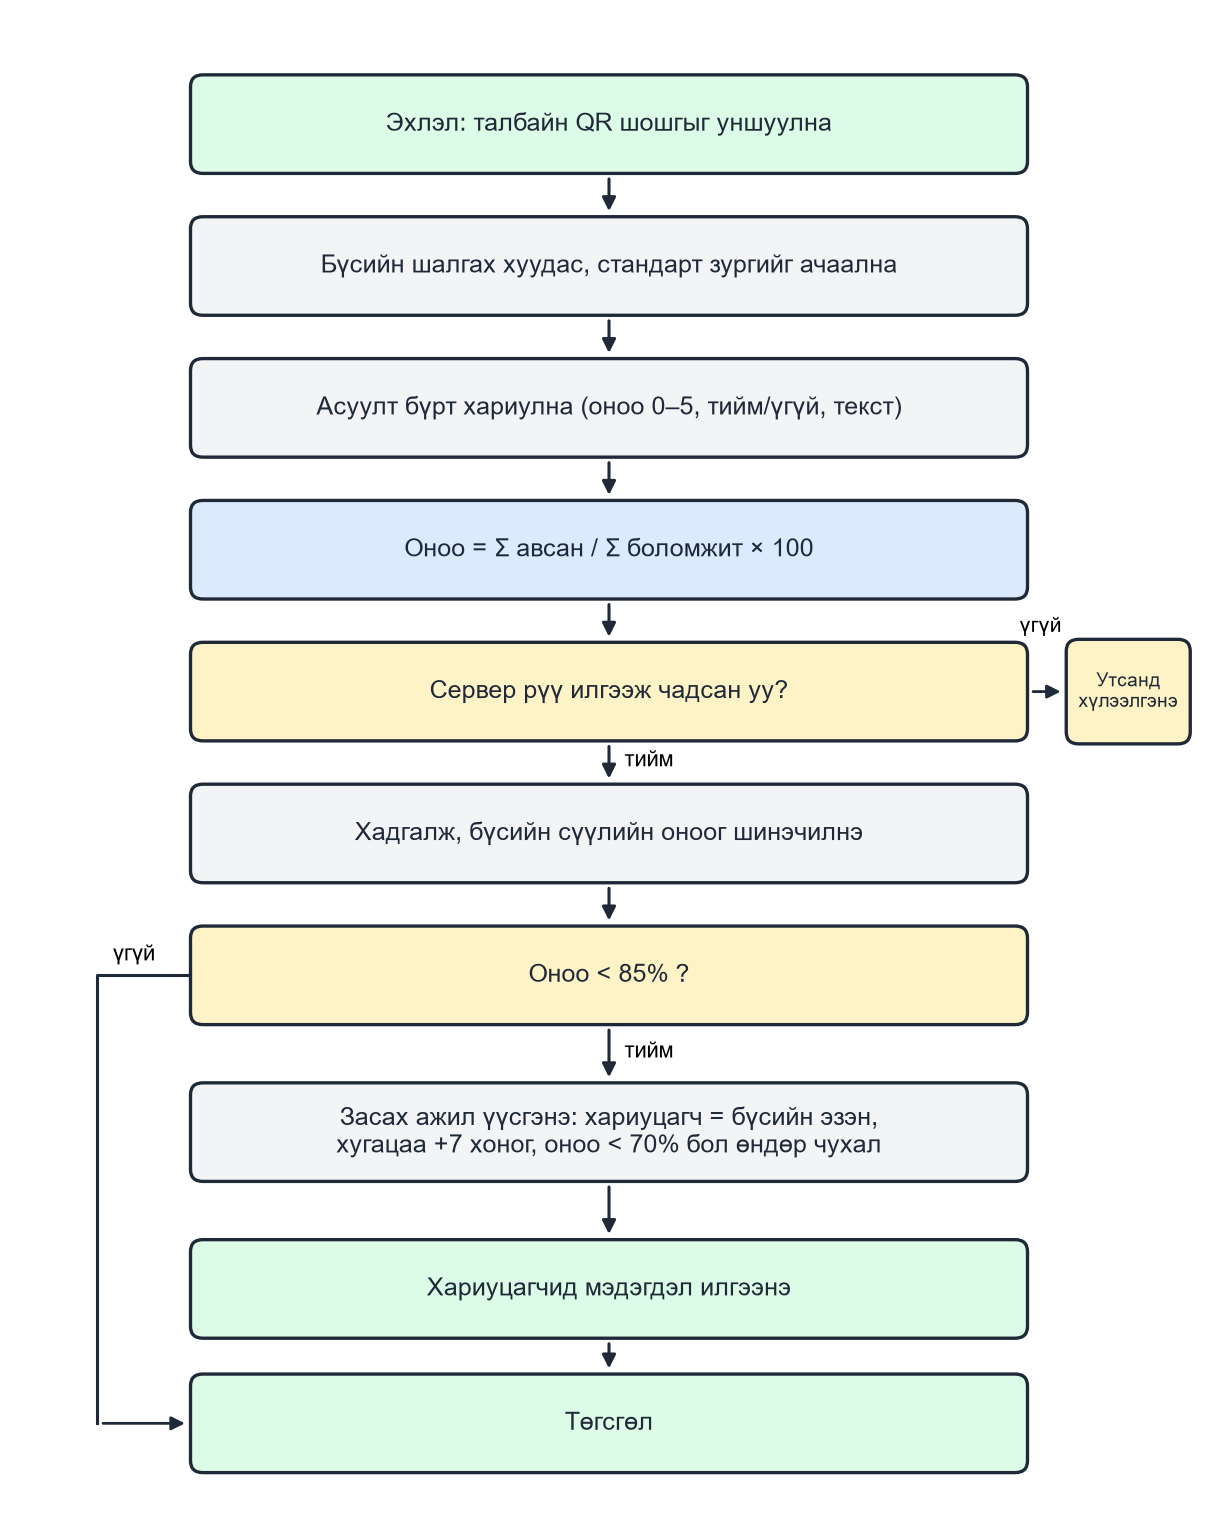
\includegraphics[width=0.62\linewidth]{Figures/audit_flow.png}
\caption{5S аудитын алгоритмын урсгал}
\label{fig:auditflow}
\end{figure}

\subsection{Сүлжээгүй горимын дараалал (outbox)}
5S аудит хийгддэг агуулах, цех, подвал зэрэг газарт сүлжээ тасалдах нь элбэг. Гар утасны апп илгээж чадаагүй бичилтийг хийсэн дарааллаар нь утасны санах ойд хадгалж, сүлжээ сэргэх, апп дахин нээгдэх эсвэл хэрэглэгч ``Одоо илгээх'' дарах үед илгээнэ (Зураг~\ref{fig:outbox}). Гол асуудал нь давхар бүртгэл: хариу ирээгүй хүсэлт серверт хүрсэн байж болно. Иймд зөвхөн серверт огт хүрээгүй нь тодорхой (холболт тогтоогдоогүй) хүсэлтийг дараалалд хийнэ; timeout-ыг дахин илгээхгүй. Дарааллыг илгээх үед сервер 4xx хариугаар татгалзвал тэр бичилтийг хасч хэрэглэгчид мэдэгдэнэ; сервер алдаатай (5xx) эсвэл нэвтрэлт дууссан бол хадгалаад дараа дахин оролдоно.

\begin{figure}[H]
\centering
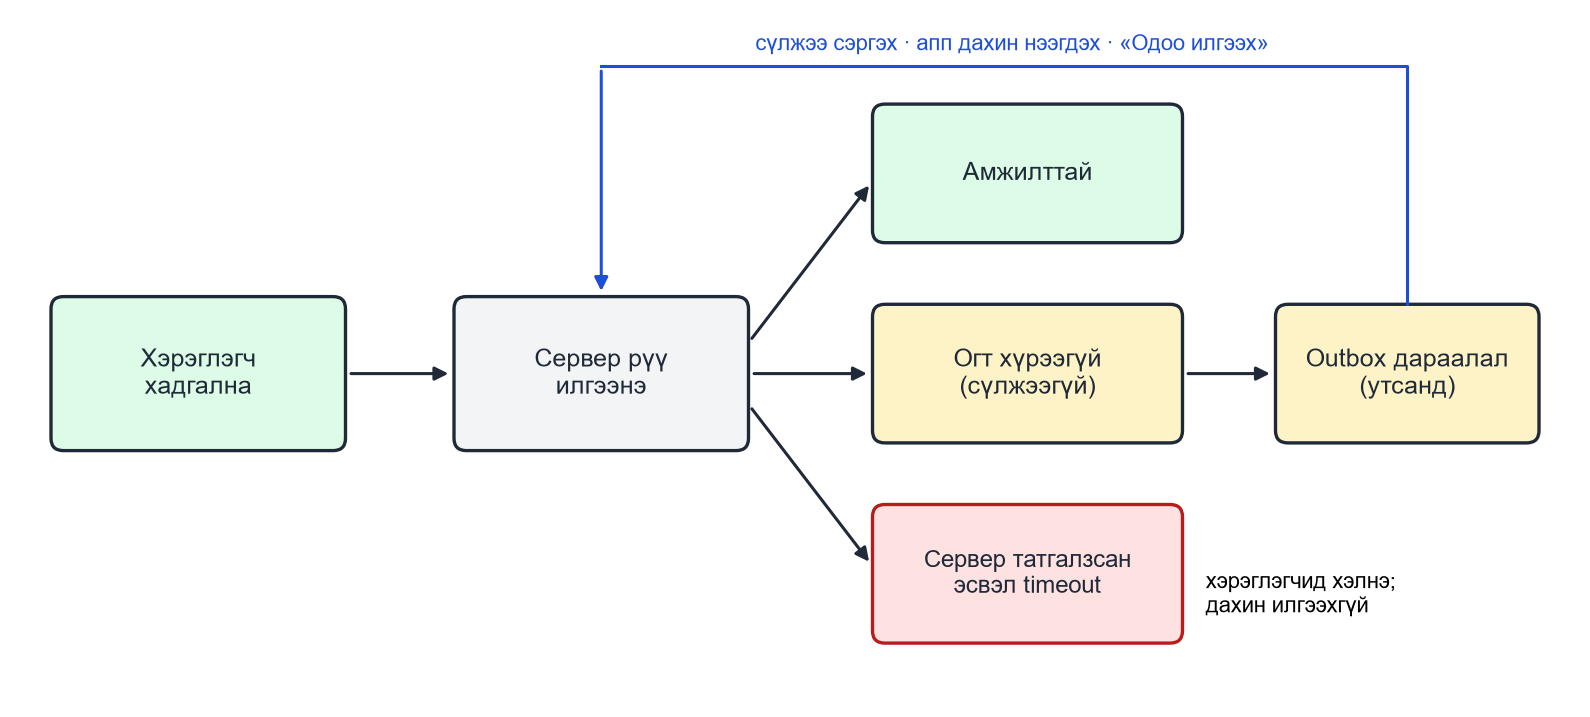
\includegraphics[width=0.9\linewidth]{Figures/outbox.png}
\caption{Сүлжээгүй горимын дарааллын урсгал}
\label{fig:outbox}
\end{figure}

\begin{lstlisting}[caption={Outbox дараалал},label={lst:outbox}]
function save(write):
    try: api.send(write)
    catch error:
        if neverSent(error): outbox.append(write)    // no connection
        else: throw error                           // timeout, 4xx, 5xx

function flush():                                   // network back / app opened
    for write in outbox (in order):
        try: api.send(write); outbox.remove(write)
        catch error:
            if no response or status >= 500 or status == 401: break   // retry later
            outbox.remove(write); refused += 1       // 4xx: final answer
\end{lstlisting}

\subsection{Өдрийн сануулга}
Өглөө бүр ажилтанд тухайн өдөр дуусах болон хоцорсон ажлын жагсаалт, менежерт багийн хоцорсон болон хариуцагчгүй ажлын жагсаалт илгээгдэнэ. Сервер UTC цагаар ажилладаг тул тооцоог байгууллагын цагийн бүсээр хийнэ. Cron цаг тутам ажиллаж, тохируулсан цагаас хойш үдээс өмнөх эхний ажиллалтаар илгээнэ. Мэдэгдлийн эх сурвалж нь тухайн өдөр тул нэг хүнд өдөрт нэгээс илүү сануулга очихгүй (idempotent).

\begin{lstlisting}[caption={Өдрийн сануулга},label={lst:remind}]
every hour:
    for org in organizations:
        tz = org.timeZone; hour = localHour(tz, now)
        if hour < org.reminderHour or hour >= 12: continue
        day = localDate(tz, now)
        for person in org.activeUsers:
            due  = tasks(person) where status not in {done, backlog} and dueDate == day
            late = tasks(person) where status not in {done, backlog} and dueDate <  day
            if (due or late) and not notified(person, source = day):
                notify(person, due, late, source = day)
\end{lstlisting}

\subsection{Сарын тайлан бүрдүүлэх ба хаах}
Сарын тайлан тухайн сарын бүртгэлүүдээс (ажил, аудит, өдрийн болон цагийн бүртгэл, зардал, өдрийн зорилго, үнэлгээ) нэг функцээр тоологдоно. Сар нээлттэй байхад шууд хүснэгтүүдээс, хаагдсаны дараа хадгалсан хуулбараас тоологддог боловч дүрэм нэг тул хоёр үр дүн зөрөхгүй. Биелэлтийн хувь нь ажлын одоогийн төлвөөс бус, хэзээ дууссанаас тооцогдоно:
\begin{equation}
C = \frac{\left|\{t \in P_m : t.\mathrm{completedAt} \le \mathrm{end}(m)\}\right|}{|P_m|}
\end{equation}
энд $P_m$ -- $m$ сард төлөвлөгдсөн ажлын олонлог. Хагас жил, жилийн тайлан хаагдсан сарын тайлангуудын нийлбэр тул батлагдсан сарын тайлантай үргэлж тохирно. Тайлангийн тойм бичвэрийг менежер хүсвэл Claude хэлний загвар ноороглоно~\cite{anthropic}; загвар руу зөвхөн нэгдсэн тоо, нэргүй саад бэрхшээл илгээгдэх ба ноорог менежер батлахаас нааш албан ёсны бичвэр болохгүй.

\subsection{Бүтээмжийн үзүүлэлт тооцох}
Хүснэгт~\ref{table:kpi}-ийн K1--K4 үзүүлэлтийг ажлын болон аудитын бүртгэлээс нэг дамжилтаар тооцно (Эх код~\ref{lst:kpi}). Бүх огноог байгууллагын цагийн бүсээр хөрвүүлж, хугацаа нь тухайн үед дуусах ёстой ажлыг л хуваарьт тооцно; хэн ч амлаагүй (backlog) ажлыг хасна. Тооцоо нь ажлын тоо $n$, аудитын тоо $m$-ээр $O(n + m)$ хугацаатай.

\begin{lstlisting}[caption={Бүтээмжийн үзүүлэлт (K1--K4)},label={lst:kpi}]
function kpis(tasks, audits, period, tz, today):
    due = [t for t in tasks if t.status != backlog and t.dueDate in period]
    onTime = [t for t in due if t.completedAt and localDate(t.completedAt, tz) <= t.dueDate]
    K1 = 100 * len(onTime) / len(due)                     // if due is empty: none
    late = [t for t in tasks if t.status not in {done, backlog} and t.dueDate < today]
    K2 = (len(late), mean(today - t.dueDate for t in late))
    runs = [a for a in audits if a.status == done and a.date in period]
    K3 = (mean(a.score for a in runs), share of zones whose last score >= 85)
    fixes = [t for t in tasks if t.sourceType == audit_run and t.completedAt in period]
    K4 = mean(days(t.completedAt - t.createdAt) for t in fixes)
    return K1, K2, K3, K4
\end{lstlisting}

\subsection{Ажлыг ач холбогдлоор бүлэглэх}
Ажилтны ажлын жагсаалт ``хоцорсон $\rightarrow$ өнөөдөр $\rightarrow$ энэ долоо хоног $\rightarrow$ дараа $\rightarrow$ хугацаагүй $\rightarrow$ дууссан'' дарааллаар бүлэглэгдэнэ. Хэн ч амлаагүй (backlog) ажил хоцордоггүй. Алгоритм нэг дамжилтаар $O(n)$ хугацаанд ажиллана.

%-------------------------------------------------------------------------------
\section{Хэрэглэгчийн интерфейс}
Интерфейсийг зорилгоор нь бүлэглэсэн цэсээр (Миний өдөр, Баг, Ажил, 5S ба аудит, Санаа, Мэдэгдэл, Тайлан, Хүмүүс, Тохиргоо) зохион байгуулав. Өглөөний хурлын самбар тоо баримтыг холоос уншигдахуйц том үсгээр, бүтэн дэлгэцээр харуулна (Зураг~\ref{fig:huddle}).

\begin{figure}[H]
\centering
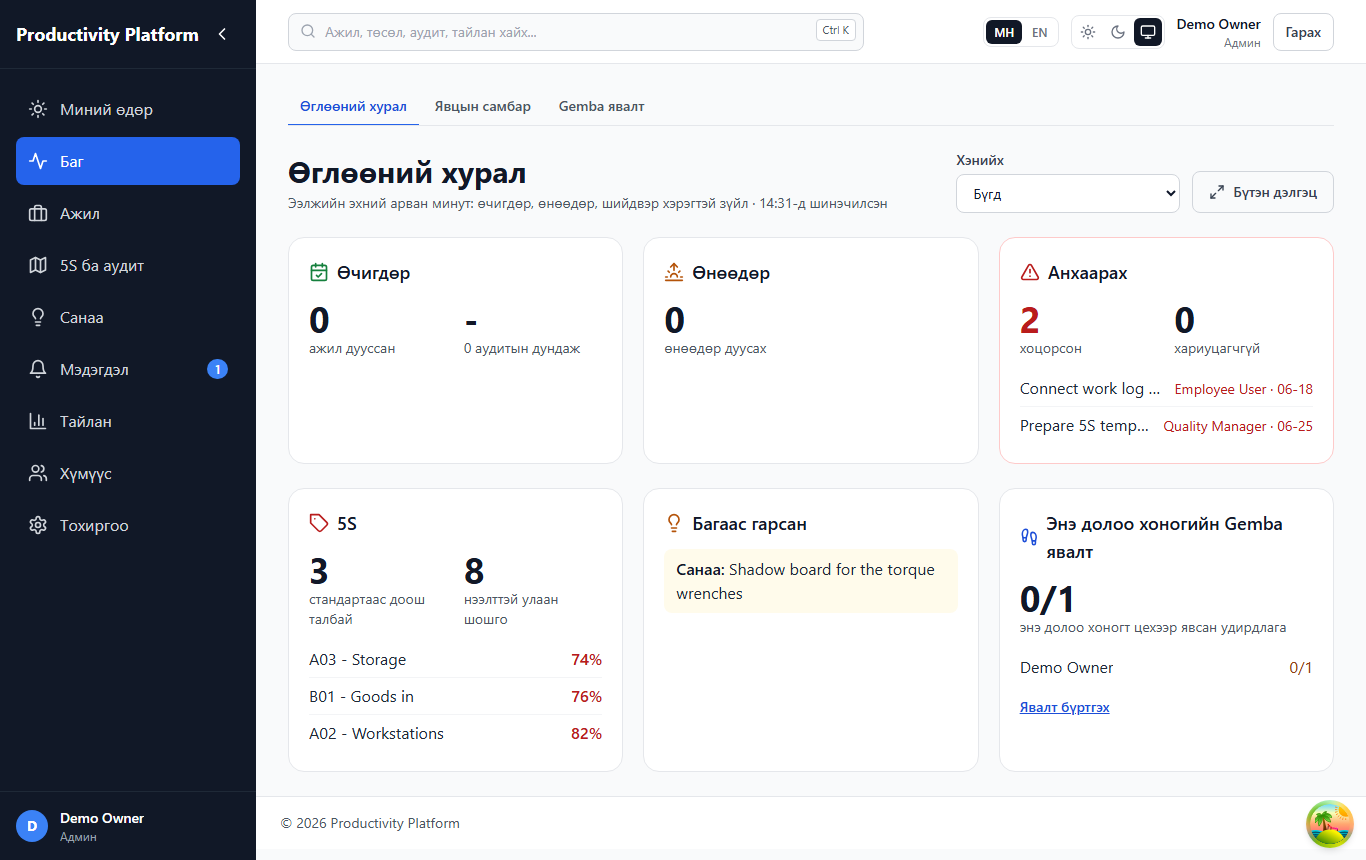
\includegraphics[width=\linewidth]{Figures/ui_huddle.png}
\caption{Өглөөний хурлын самбар}
\label{fig:huddle}
\end{figure}

\begin{figure}[H]
\centering
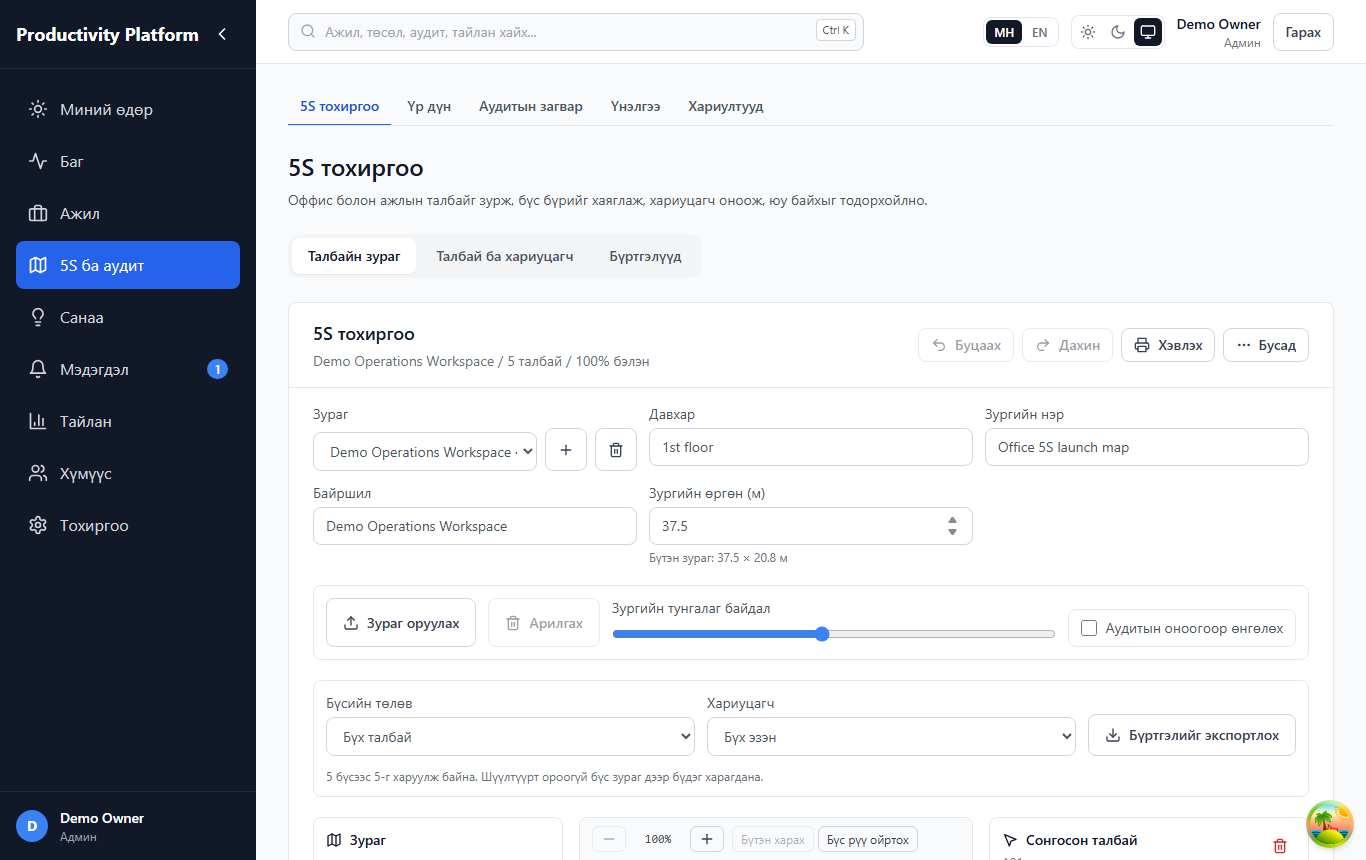
\includegraphics[width=\linewidth]{Figures/ui_fives.png}
\caption{5S талбайн зураг ба бүсийн тохиргоо}
\label{fig:fives}
\end{figure}

Ажилтны нүүр хуудас ``Миний өдөр'' нь тухайн өдрийн ажил, хоцорсон ажил, мэдэгдэл, долоо хоногийн тайлангийн сануулгыг нэг дор харуулна (Зураг~\ref{fig:dashboard}). Ажлын хуудас ажлыг төлөв, хариуцагч, хугацаагаар шүүж харуулна (Зураг~\ref{fig:tasksui}).

\begin{figure}[H]
\centering
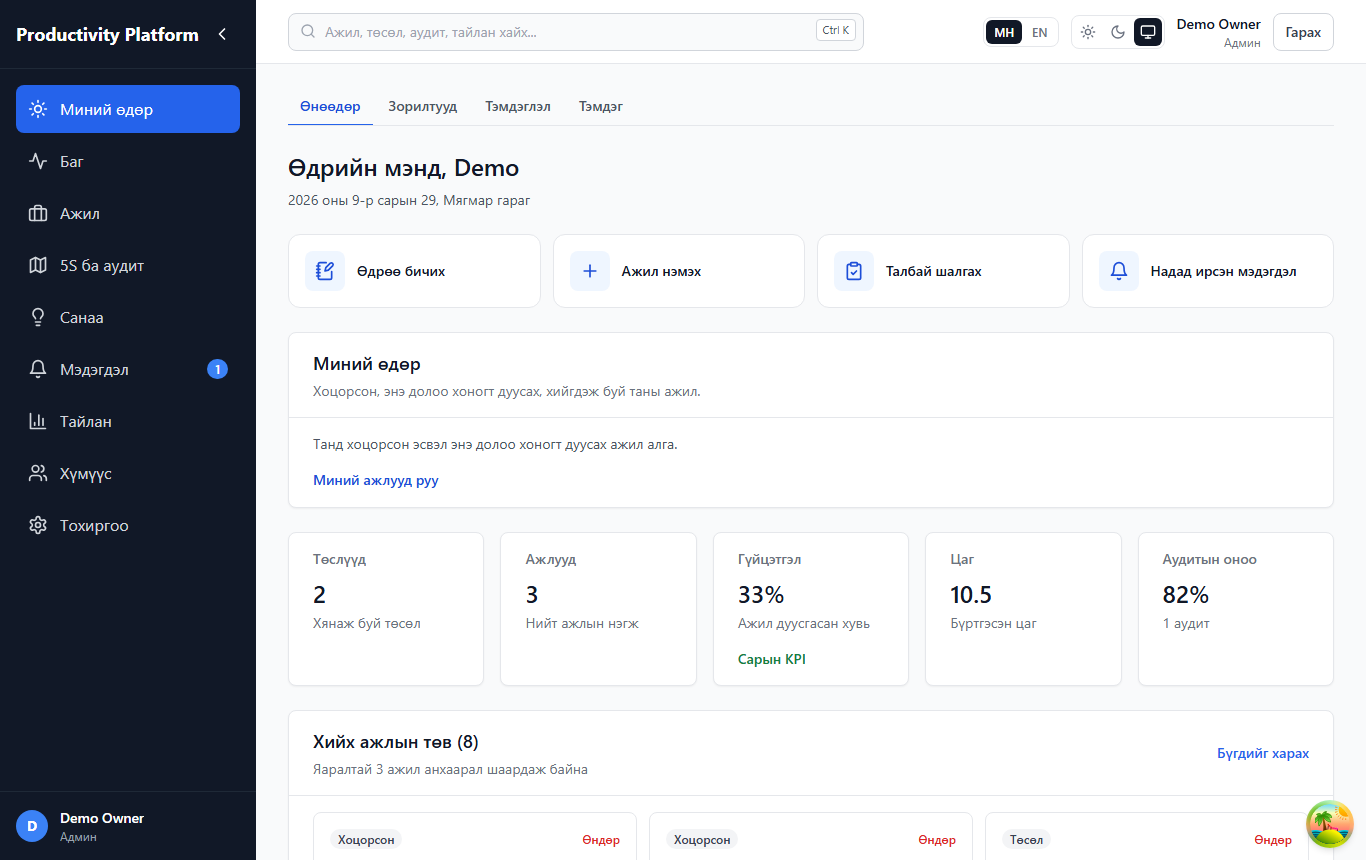
\includegraphics[width=\linewidth]{Figures/ui_dashboard.png}
\caption{``Миний өдөр'' нүүр хуудас}
\label{fig:dashboard}
\end{figure}

\begin{figure}[H]
\centering
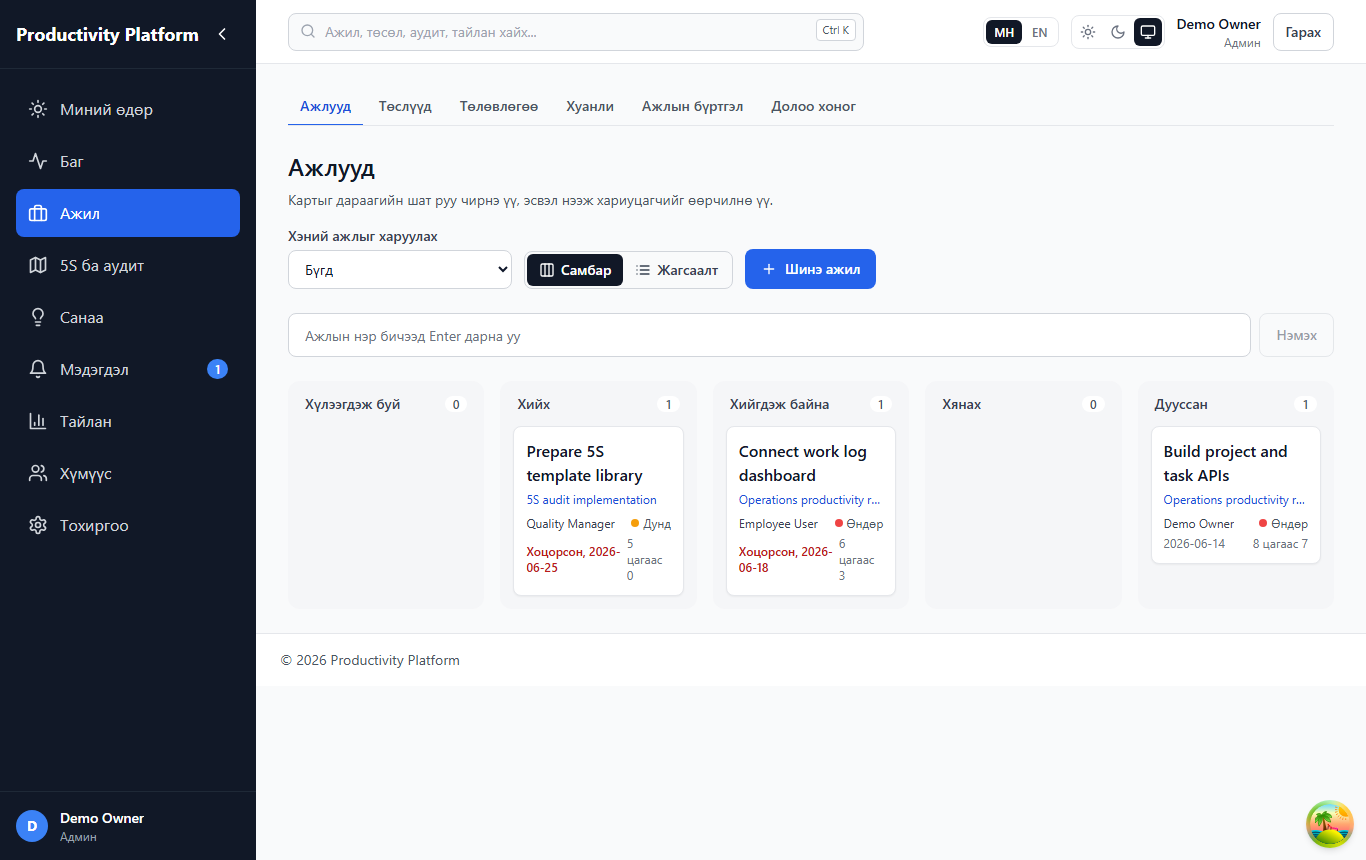
\includegraphics[width=\linewidth]{Figures/ui_tasks.png}
\caption{Ажлын жагсаалт}
\label{fig:tasksui}
\end{figure}

Сарын тайлан бүртгэлээс автоматаар бүрдэх бөгөөд менежер тойм бичвэрийг бичиж эсвэл AI-аар ноороглуулж батална (Зураг~\ref{fig:reportui}). Gemba явалтын хуудсанд менежер ажигласан зүйл, дараагийн алхмуудаа бүртгэж, долоо хоногийн зорилтын биелэлтийг харна (Зураг~\ref{fig:gembaui}).

\begin{figure}[H]
\centering
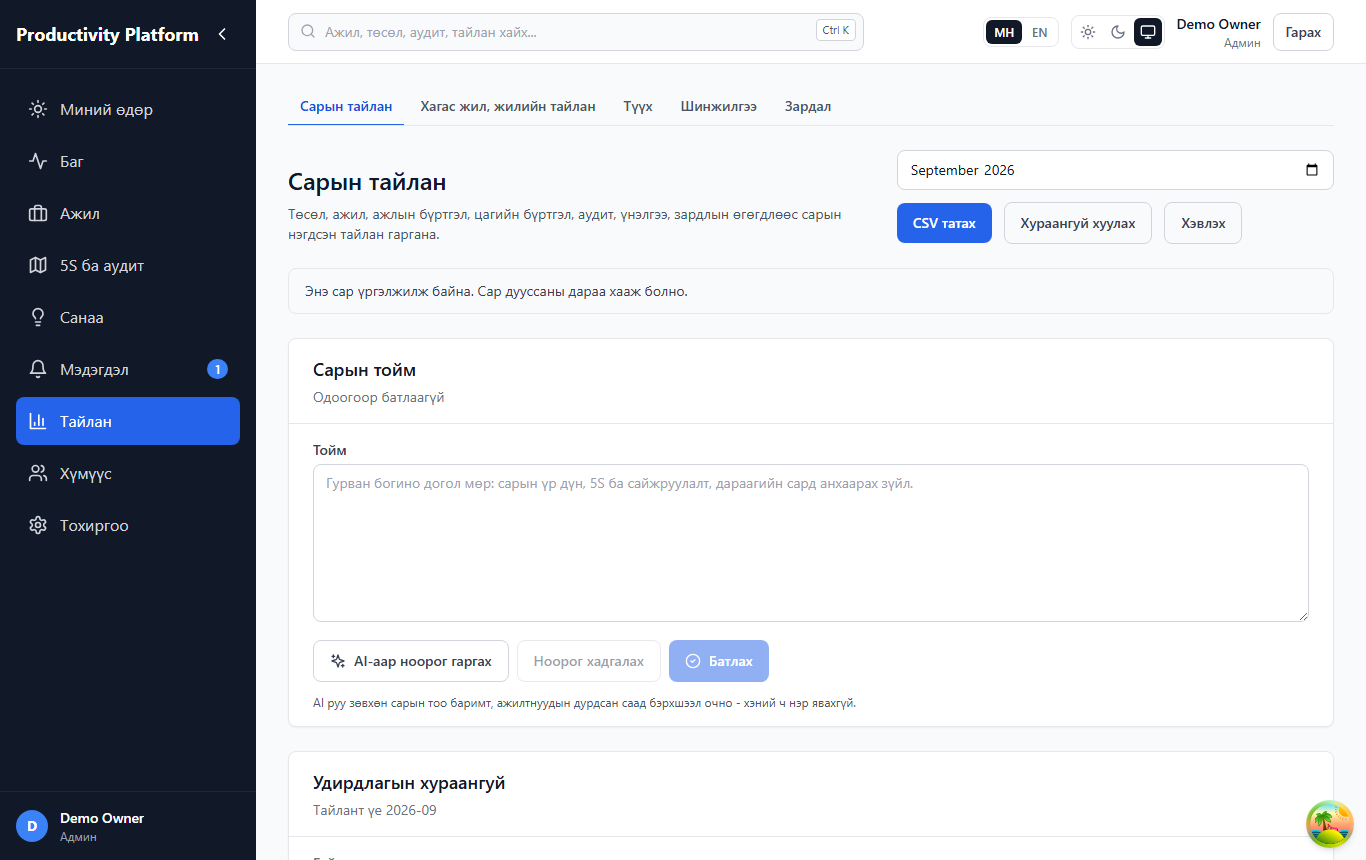
\includegraphics[width=\linewidth]{Figures/ui_report.png}
\caption{Сарын тайлан}
\label{fig:reportui}
\end{figure}

\begin{figure}[H]
\centering
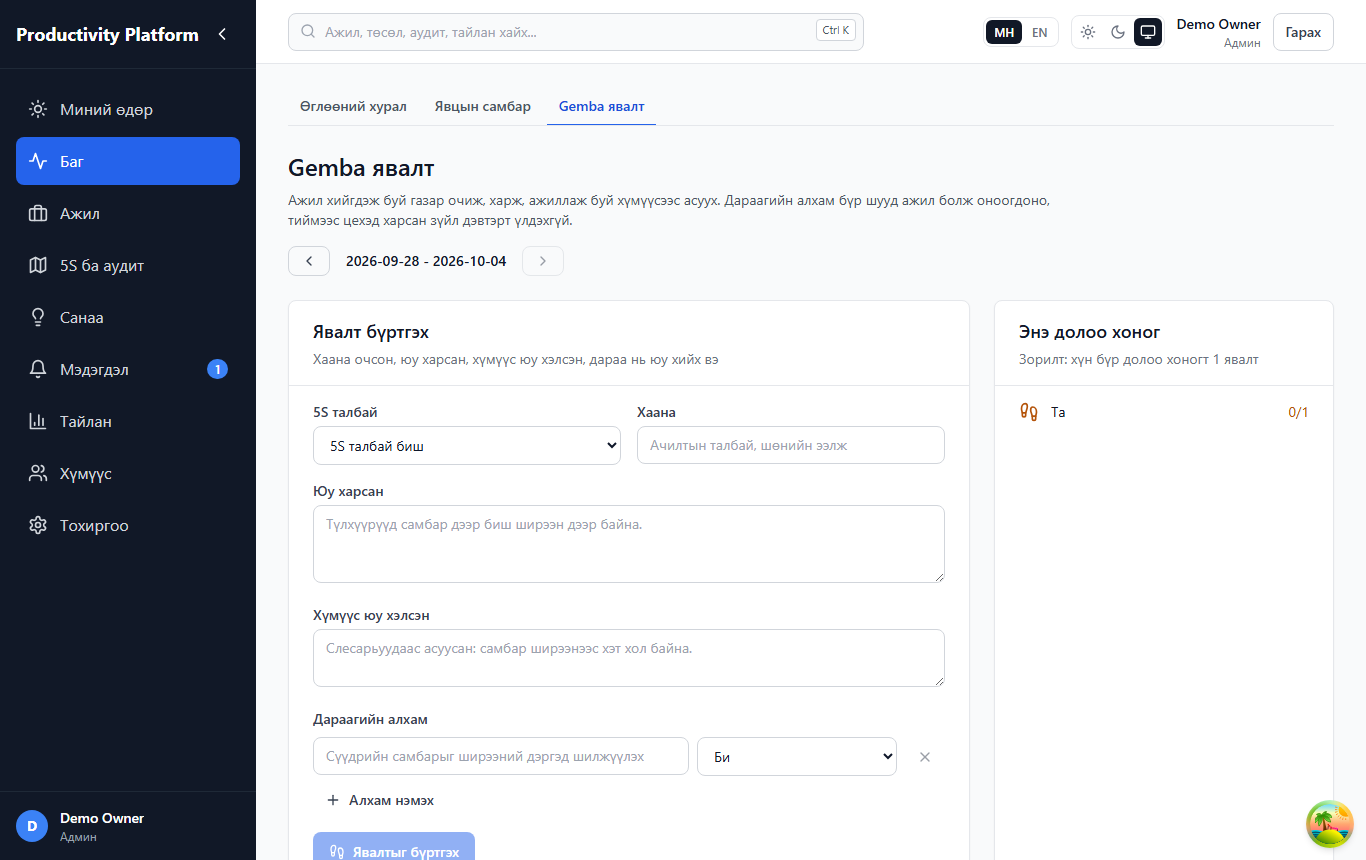
\includegraphics[width=\linewidth]{Figures/ui_gemba.png}
\caption{Gemba явалт бүртгэх}
\label{fig:gembaui}
\end{figure}

Гар утасны апп цех дээрх ажилтанд зориулагдсан. ``Миний ажлууд'' таб ажлыг хоцорсон, өнөөдөр, энэ долоо хоногт гэж бүлэглэж, нэг товшилтоор дуусгах боломж олгоно. 5S табаас талбайг сонгох эсвэл QR шошго уншуулж шалгах хуудсаар аудит хийж, улаан шошго бүртгэнэ. Мэдэгдлийн табаас ирсэн мэдэгдлийг цагтай нь харж, холбогдох таб руу шууд шилжинэ (Зураг~\ref{fig:mobileui}).

\begin{figure}[H]
\centering
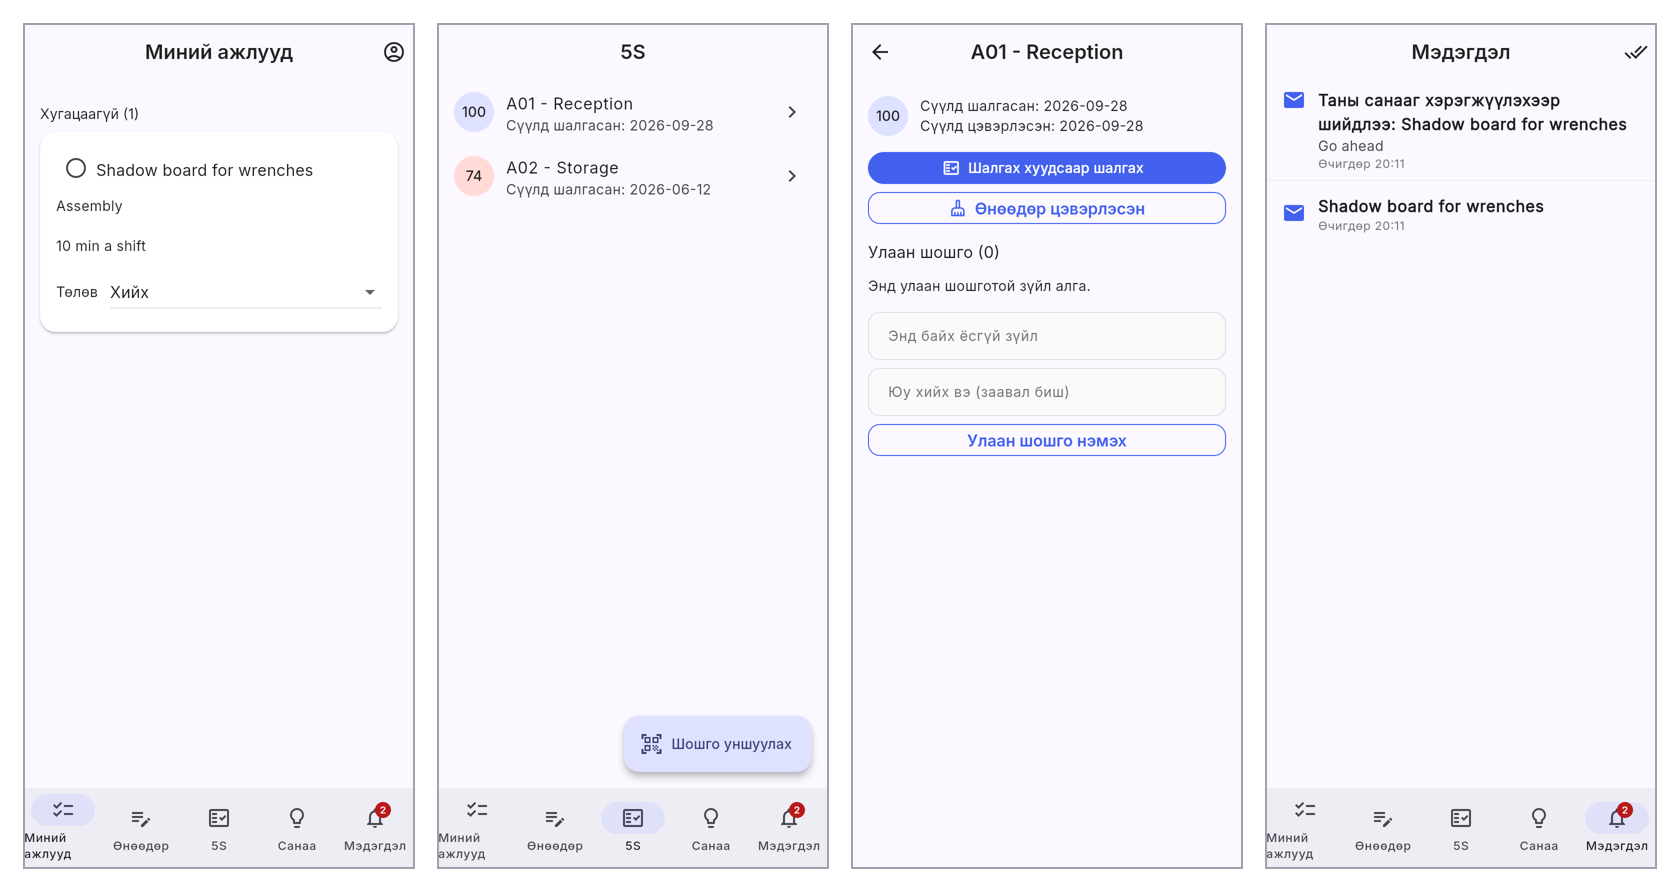
\includegraphics[width=\linewidth]{Figures/ui_mobile.png}
\caption{Гар утасны апп: ажил, 5S талбай, бүс, мэдэгдэл}
\label{fig:mobileui}
\end{figure}

%-------------------------------------------------------------------------------
\section{Системийн туршилтын загвар боловсруулах}
Системийг гурван түвшинд автоматаар туршина (Хүснэгт~\ref{table:tests}). Өөрчлөлт бүрийн дараа бүх тест ажиллаж, амжилтгүй тест байвал өөрчлөлтийг нэгтгэхгүй.

\begin{table}[H]
\centering
\caption{Туршилтын түвшин}
\label{table:tests}
\begin{tabular}{|p{3.2cm}|p{6.4cm}|p{4.6cm}|}
\hline
\textbf{Түвшин} & \textbf{Юуг шалгах} & \textbf{Хэрэгсэл, тоо} \\ \hline
Unit & Оноо тооцох, бүлэглэх, эрх шалгах зэрэг функц & Jest, Vitest, flutter\_test \\ \hline
Integration & API маршрут, өгөгдлийн сан, эрхийн guard & Jest (backend 830 тест) \\ \hline
Component & Вэб хуудас, компонент, орчуулга & Vitest (1017 тест) \\ \hline
End-to-end & Хөтөч дээр бүтэн урсгал, WCAG хүртээмж & Playwright + axe (39 тест) \\ \hline
Гар утас & Дэлгэц, outbox, том үсэг, хүртээмж & flutter\_test (116 тест) \\ \hline
\end{tabular}
\end{table}

Гол туршилтын тохиолдлууд:
\begin{enumerate}[label=(\alph*)]
    \item Нэвтрэх -- зөв, буруу нууц үг, идэвхгүй бүртгэл.
    \item 5S аудит -- оноо 85\%-иас доош бол засах ажил нэг удаа үүсэх; дахин илгээхэд давхардахгүй.
    \item Сүлжээгүй горим -- сүлжээгүй үед хадгалагдаж, сүлжээ сэргэхэд илгээгдэх; 4xx хариуг дахин илгээхгүй.
    \item Эрх -- ажиглагч ажил устгах хүсэлт илгээхэд 403 буцах.
    \item Сарын тайлан -- хаагдсан сарын тайлан дараа нь өгөгдөл өөрчлөгдсөн ч хэвээр байх.
\end{enumerate}

\section*{Бүлгийн дүгнэлт}
Энэ бүлэгт системийн давхаргат архитектур, зохиомжийн класс, дарааллын диаграмм, өгөгдлийн сангийн схем, эрхийн загварыг боловсруулав. Аудитын оноо ба засах ажил, сүлжээгүй горимын дараалал, өдрийн сануулга, сарын тайлан, бүтээмжийн үзүүлэлт, ажлын бүлэглэлт гэсэн зургаан алгоритмыг зохиомжилж, байршуулалтын диаграмм болон туршилтын загварыг тодорхойлов.

% Бүлэг 4

\chapter{Эдийн засгийн үр ашгийн тооцоо}
\label{Chapter4}

\section{Төслийн эдийн засгийн үр ашгийн шинжилгээ}
Мэдээллийн системийн төслийг зөвхөн техникийн хэрэгжилтээр бус, эдийн засгийн үр ашгийн үзүүлэлтээр үнэлэх шаардлагатай. Энэхүү систем нь байгууллагын дотоод хэрэгсэл тул түүний өгөөж нь борлуулалтын орлого бус, ажилтнуудын хэмнэсэн ажлын цагийн үнэлгээ юм. Иймд үр ашгийг 25 ажилтантай (үүнээс 5 менежер) жишээ байгууллагын хэмжээнд, мөнгөний цаг хугацааны үнэ цэнийг тооцсон аргуудаар (NPV, нөхөх хугацаа) болон ашигт ажиллагаа, зардлын түвшин, бүтээмжийн үзүүлэлтүүдээр тооцов.

\subsection{Тооцоололд ашигласан томьёонууд}
Мөнгөний өнөөгийн үнэ цэнэ (PV):
\begin{equation}
PV = \frac{FV}{(1+r)^n}
\end{equation}
Хөрөнгө оруулалтын өнөөгийн цэвэр үнэ цэнэ (NPV):
\begin{equation}
NPV = \sum_{i=1}^{n} \frac{FV_i}{(1+r)^i} - Inv
\end{equation}
энд $FV_i$ -- $i$-р жилийн цэвэр мөнгөн урсгал, $r$ -- хорогдлын хувь, $n$ -- хугацаа, $Inv$ -- анхны хөрөнгө оруулалт.

Хөрөнгө оруулалтыг нөхөх хугацаа:
\begin{equation}
T_{inv} = t + \frac{Inv - \sum_{i=1}^{t} PV_i}{PV_{t+1}}
\end{equation}
Хөрөнгө оруулалтын үр ашгийн дундаж норм:
\begin{equation}
PfN = \frac{\left(\sum_{i=1}^{n} PV_i\right)/n}{Inv}
\end{equation}
Ашигт ажиллагаа, зардлын түвшин, нийт бүтээмж:
\begin{equation}
P_a = \frac{Profit}{Income}\times 100\%, \quad
P_c = \frac{Profit}{Inv}, \quad
Z_t = \frac{Cost}{Income}\times 100\%, \quad
TP = \frac{Income}{Cost}
\end{equation}

\subsection{Тооцооллын суурь өгөгдөл, таамаглал}
% Эдгээр нь таамаглал. Туршилтын байгууллагын бодит тоо (ажилтны тоо, цалин,
% хэмнэсэн цаг)-г авсны дараа шинэчилнэ.
\begin{itemize}
    \item Ашиглалтын хугацаа $n = 5$ жил, хорогдлын хувь $r = 12\%$.
    \item Ажилтны нэг цагийн дундаж өртөг 12\,000 төгрөг.
    \item Ажилтан бүр ажлын явц тодруулах, мэдээлэл хайх, тайлагнахад долоо хоногт 2 цаг хэмнэнэ: $25 \times 2 \times 48 = 2\,400$ цаг/жил.
    \item Менежер бүр ажил хянах, мэдээлэл нэгтгэхэд долоо хоногт 3 цаг хэмнэнэ: $5 \times 3 \times 48 = 720$ цаг/жил.
    \item Сарын тайлан бэлтгэх 24 цаг автоматжина: $24 \times 12 = 288$ цаг/жил.
    \item Нийт хэмнэлт 3\,408 цаг/жил; жилийн өгөөж $Income = 3\,408 \times 12\,000 = 40\,896\,000$ төгрөг.
    \item Жилийн зардал $Cost = 6\,900\,000$ төгрөг (засвар үйлчилгээ 6\,000\,000, сервер 600\,000, AI үйлчилгээ 300\,000).
    \item Жилийн цэвэр мөнгөн урсгал $Profit = Income - Cost = 33\,996\,000$ төгрөг.
\end{itemize}

\subsection{Анхны хөрөнгө оруулалтын зардал}
\begin{table}[H]
\centering
\caption{Анхны хөрөнгө оруулалтын бүтэц}
\label{table:inv}
\begin{tabular}{|p{8cm}|r|}
\hline
\textbf{Зардлын төрөл} & \textbf{Дүн (төгрөг)} \\ \hline
Судалгаа, системийн загварчлал & 3\,000\,000 \\ \hline
Backend, вэб, гар утасны хөгжүүлэлт (6 сар) & 18\,000\,000 \\ \hline
Тестлэлт, баримтжуулалт & 2\,000\,000 \\ \hline
Сервер, дэд бүтэц, апп дэлгүүрийн бүртгэл & 1\,000\,000 \\ \hline
\textbf{Нийт (Inv)} & \textbf{24\,000\,000} \\ \hline
\end{tabular}
\end{table}

\subsection{NPV тооцоолол}
\begin{table}[H]
\centering
\caption{NPV тооцооллын хүснэгт ($r = 12\%$, $FV_i = 33\,996\,000$ төгрөг)}
\label{table:npv}
\begin{tabular}{|c|r|c|r|}
\hline
\textbf{Жил} & \textbf{$FV_i$ (төгрөг)} & \textbf{$(1+r)^i$} & \textbf{$PV_i$ (төгрөг)} \\ \hline
1 & 33\,996\,000 & 1.12000 & 30\,353\,571 \\ \hline
2 & 33\,996\,000 & 1.25440 & 27\,101\,403 \\ \hline
3 & 33\,996\,000 & 1.40493 & 24\,197\,681 \\ \hline
4 & 33\,996\,000 & 1.57352 & 21\,605\,073 \\ \hline
5 & 33\,996\,000 & 1.76234 & 19\,290\,243 \\ \hline
\multicolumn{3}{|r|}{$\sum PV_i$} & 122\,547\,972 \\ \hline
\end{tabular}
\end{table}

\begin{equation}
NPV = 122\,547\,972 - 24\,000\,000 = 98\,547\,972 \text{ төгрөг}
\end{equation}
$NPV > 0$ тул төсөл эдийн засгийн хувьд үр ашигтай.

\subsection{Хөрөнгө оруулалтыг нөхөх хугацаа}
Эхний жилийн $PV_1 = 30\,353\,571$ төгрөг нь $Inv = 24\,000\,000$ төгрөгөөс их тул:
\begin{equation}
T_{inv} = 0 + \frac{24\,000\,000}{30\,353\,571} \approx 0.79 \text{ жил} \approx 9.5 \text{ сар}
\end{equation}

\subsection{Бусад үзүүлэлт}
\begin{equation}
PfN = \frac{122\,547\,972 / 5}{24\,000\,000} \approx 1.02, \qquad
P_a = \frac{33\,996\,000}{40\,896\,000}\times 100\% \approx 83.13\%
\end{equation}
\begin{equation}
P_c = \frac{33\,996\,000}{24\,000\,000} \approx 1.42, \qquad
Z_t = \frac{6\,900\,000}{40\,896\,000}\times 100\% \approx 16.87\%, \qquad
TP = \frac{40\,896\,000}{6\,900\,000} \approx 5.93
\end{equation}

\section{Эдийн засгийн үзүүлэлтүүдийн нэгдсэн дүн}
\begin{table}[H]
\centering
\caption{Эдийн засгийн үзүүлэлтүүдийн нэгдсэн дүн}
\label{table:econ}
\begin{tabular}{|p{8cm}|r|}
\hline
\textbf{Үзүүлэлт} & \textbf{Үр дүн} \\ \hline
Анхны хөрөнгө оруулалт (Inv) & 24\,000\,000 төгрөг \\ \hline
Жилийн өгөөж (хэмнэсэн цагийн үнэлгээ) & 40\,896\,000 төгрөг \\ \hline
Жилийн зардал & 6\,900\,000 төгрөг \\ \hline
Жилийн цэвэр мөнгөн урсгал & 33\,996\,000 төгрөг \\ \hline
NPV (5 жил, $r = 12\%$) & 98\,547\,972 төгрөг \\ \hline
Нөхөх хугацаа & $\approx$ 0.79 жил (9.5 сар) \\ \hline
Үр ашгийн дундаж норм (PfN) & 1.02 \\ \hline
Ашигт ажиллагаа ($P_a$) & 83.13\% \\ \hline
Зардлын түвшин ($Z_t$) & 16.87\% \\ \hline
Нийт бүтээмж (TP) & 5.93 \\ \hline
\end{tabular}
\end{table}

\section*{Бүлгийн дүгнэлт}
Тооцооллоор системийн NPV эерэг, хөрөнгө оруулалт нэг жилд хүрэхгүй хугацаанд нөхөгдөж, нэг төгрөгийн зардлаар 5.93 төгрөгийн өгөөж бий болох боломжтой байна. Тооцоо нь хэмнэгдэх ажлын цагийн таамаглалд суурилсан тул туршилтын ажиллагааны үед бодит хэмнэлтийг хэмжиж шинэчилнэ.

\pagestyle{plain}
% Ерөнхий дүгнэлт

\phantomsection
\addchaptertocentry{Ерөнхий дүгнэлт}
\label{Summary}
\section*{Ерөнхий дүгнэлт}
Энэхүү дипломын ажлын хүрээнд байгууллагын 5S, бүтээмжийн хэрэгслүүд болон ажлын удирдлагыг нэгтгэсэн вэб, гар утасны платформыг зохион бүтээв. Үүнд:
\begin{itemize}
    \item lean, 5S, Gemba, Kaizen, шатлалт өдөр тутмын хурлын онолыг судалж, хэрэгслийг дадал болгоход сануулга, хяналтын механизм шаардлагатайг тодорхойлсон;
    \item ижил төстэй таван системийг харьцуулж, аудит, ажлын удирдлага, lean дадлыг нэг дор, монгол хэл дээр нэгтгэсэн шийдэл байхгүйг тогтоосон;
    \item бүтээмжийг хэмжих долоон үзүүлэлт ба ``өмнө--дараа'' үнэлгээний загварыг тодорхойлсон;
    \item 22 функциональ, 10 функциональ бус шаардлага, есөн use-case-ийн тодорхойлолт, шаардлагын мөрдөх матриц, класс, дараалал, үйл ажиллагааны диаграмм боловсруулсан;
    \item давхаргат архитектур, байршуулалтын диаграмм, 25 хүснэгттэй өгөгдлийн сан, дүрд суурилсан эрхийн загвар, зургаан гол алгоритмыг зохиомжилсон;
    \item backend, вэб, гар утасны аппыг хөгжүүлж, 2\,000 гаруй автомат тестээр баталгаажуулсан;
    \item таамаглалд суурилсан урьдчилсан эдийн засгийн тооцоо хийж, бодит үр ашгийг туршилтын ажиллагаагаар шалгахаар төлөвлөсөн.
\end{itemize}

Ажлын одоогийн төлөвийг гурван түвшинд ялгаж харуулав (Хүснэгт~\ref{table:status}). Системийн гол урсгалууд кодонд хэрэгжиж, автомат тестээр баталгаажсан боловч бодит байгууллагад ашиглаж бүтээмжийн өөрчлөлтийг хэмжих ажил хараахан хийгдээгүй; энэ нь дараагийн үзлэгүүдийн гол ажил юм.

\begin{table}[H]
\centering
\caption{Ажлын гүйцэтгэлийн төлөв}
\label{table:status}
\begin{tabular}{|p{5.6cm}|>{\centering\arraybackslash}p{2.6cm}|>{\centering\arraybackslash}p{2.6cm}|>{\centering\arraybackslash}p{2.6cm}|}
\hline
\textbf{Хэсэг} & \textbf{Кодонд хэрэгжсэн} & \textbf{Тестээр шалгасан} & \textbf{Туршилтаар хэмжсэн} \\ \hline
Ажил, төсөл, мэдэгдэл & \yes & \yes & -- \\ \hline
5S талбай, аудит, засах ажил & \yes & \yes & -- \\ \hline
Өдрийн ба долоо хоногийн тайлан & \yes & \yes & -- \\ \hline
Сарын тайлан, хаалт, архив & \yes & \yes & -- \\ \hline
Gemba, санаа, өглөөний хурал & \yes & \yes & -- \\ \hline
Сүлжээгүй горим (бичих) & $\sim$ & \yes & -- \\ \hline
KPI самбар (K1--K6) & $\sim$ & $\sim$ & -- \\ \hline
Хэрэглэгчийн судалгаа, SUS & -- & -- & -- \\ \hline
\end{tabular}
\end{table}

% TODO (Үзлэг 3): туршилтын ажиллагааны үр дүн, SUS оноо, цаашдын хөгжүүлэлтийг нэмнэ.
Цаашид системийг серверт байршуулж, туршилтын байгууллагад ажиллуулан хэрэглэхэд хялбар байдлыг SUS аргаар үнэлж, бодит хэмнэлтийг хэмжих, push мэдэгдэл нэмэх, апп дэлгүүрт нийтлэх ажлыг гүйцэтгэнэ.


\appendix
% \include{Appendices/AppendixA}

\defformat
\addchaptertocentry{Ном зүй}
\printbibliography[heading=bibliography,title={Ном зүй}]

\end{document}
